\chapter{Beyond the Standard Model  Physics Program }
\label{ch:bsm}
%%%%%%%%%%%%%%%%%%%%%%%%%%%%%%%%%%%%%%%%
\section{Executive Summary}
\label{phys:bsm:execsumm}

The unique combination of the high-intensity LBNF neutrino beam with DUNE's \dword{nd}  and massive LArTPC \dword{fd} modules at a \SI{1300}{km} baseline enables a variety of probes of beyond the standard model \dword{bsm} physics, either novel or with unprecedented sensitivity. This section describes a selection of such topics, and briefly summarizes how DUNE can make leading contributions in this arena.

\textit{Search for active-sterile neutrino mixing:} Experimental results in tension with the three-neutrino-flavor paradigm, which may be interpreted as mixing between the known active neutrinos and one or more sterile states, have led to a rich and diverse program of searches for oscillations into sterile neutrinos~\cite{ref:tension,Gariazzo:2017fdh}. DUNE is sensitive over a broad range of potential sterile neutrino mass splittings by looking for disappearance of \dword{cc} and \dword{nc}  interactions over the long distance separating the \dword{nd} and \dword{fd}, as well as over the short baseline of the \dword{nd} . With a longer baseline, a more intense beam, and a high-resolution large-mass \dword{fd}, compared to previous experiments, DUNE provides a unique opportunity to improve significantly on the sensitivities of the existing probes, and greatly enhance the ability to map the extended parameter space if a sterile neutrino is discovered.

\textit{Searches for non-unitarity of the \dword{pmns} matrix:} A generic characteristic of most models explaining the neutrino mass pattern is the presence of heavy neutrino states, additional to the three light states of the \dword{sm} of particle physics~\cite{Minkowski:1977sc,Mohapatra:1979ia,Yanagida:1979as,GellMann:1980vs}. This implies a deviation from %unitary 
unitarity of the $3 \times 3$ \dword{pmns} matrix that can %, which can be 
become particularly sizable the lower the mass of the extra states are.
For values of the unitarity deviations of order $10^{-2}$, this would decrease the expected reach of DUNE to the standard parameters, although stronger bounds existing from charged leptons would be able to restore its expected performance.

\textit{Searches for \dword{nsi}:} %non-standard neutrino interactions:} Non-standard neutrino interactions, 
\Dword{nsi} affecting neutrino propagation through the Earth, can significantly modify the data to be collected by DUNE as long as the new physics parameters are large enough~\cite{Farzan:2017xzy}. Leveraging its very long baseline and wide-band beam, DUNE is uniquely sensitive to these probes. If the DUNE data are consistent with standard oscillations for three massive neutrinos, interaction effects of order 0.1 $G_{F}$ can be ruled out at DUNE. We note that DUNE will improve current constraints on $\epsilon_{\tau e}$ and $\epsilon_{\mu e}$, the magnitude of the \dword{nsi} relative to standard weak interactions, by a factor of 2 to 5.

\textit{Searches for violation of Lorentz or \dword{cpt} Symmetry:} \dword{cpt} symmetry, the combination of charge conjugation, parity and time reversal, is a cornerstone of our model-building strategy and therefore the repercussions of its potential violation will severely threaten the \dword{sm} of particle physics~\cite{Streater:1989vi,Barenboim:2002tz,Kostelecky:2003cr,Diaz:2009qk,Kostelecky:2011gq,Barenboim:2017ewj}. DUNE can improve the present limits on Lorentz and \dword{cpt} violation by several orders of magnitude, contributing as a very important experiment to test these fundamental assumptions underlying quantum field theory.

\textit{Searches for neutrino trident production:} The intriguing possibility that neutrinos may be charged under new gauge symmetries beyond the \dword{sm}  $SU(3)_{c} \times SU(2)_{L} \times U(1)_{Y}$, and interact with the corresponding new gauge bosons can be tested with unprecedented precision by DUNE through \dword{nd}  measurements of neutrino-induced di-lepton production in the Coulomb field of a heavy nucleus, also known as neutrino trident interactions~\cite{Czyz:1964zz,Lovseth:1971vv,Fujikawa:1971nx,Koike:1971tu,Koike:1971vg,Brown:1973ih,Belusevic:1987cw}. Although this process is extremely rare (\dword{sm} rates are suppressed by a factor of $10^{-5} \-- 10^{-7}$ with respect to \dword{cc} interactions), the CHARM-II collaboration and the CCFR collaboration both reported detection of several trident events ($\sim40$ events at CCFR) and quoted cross-sections in good agreement with the \dword{sm} predictions. With a predicted annual rate of over 100 dimuon neutrino trident interactions at the \dword{nd}, DUNE will be able to measure deviations from the \dword{sm} rates and test the presence of new gauge symmetries~\cite{Altmannshofer:2019zhy,Ballett:2018uuc,Ballett:2019xoj}.

\textit{Search for \dword{ldm}:} Various cosmological and astrophysical observations strongly support the existence of \dword{dm} representing $\approx$27\% of the mass-energy of the universe, but its nature and potential non-gravitational interactions with regular matter remain undetermined~\cite{Aghanim:2018eyx}. The lack of evidence for \dwords{wimp} at direct detection and the LHC experiments has resulted in a reconsideration of the \dword{wimp} paradigm. For instance, if \dword{dm} has a mass that is much lighter than the electroweak scale (e.g., below GeV level), it motivates theories for \dword{dm} candidates that interact with ordinary matter through a new ``vector portal'' mediator. High-flux neutrino beam experiments, such as DUNE, have been shown to provide coverage of \dword{dm}+mediator parameter space that cannot be covered by either direct detection or collider experiments~\cite{Alexander:2016aln, Battaglieri:2017aum, LoSecco:1980nf, Acciarri:2015uup}. \dword{dm} particles can be detected in the \dword{nd} through neutral-current-like interactions either with electrons or nucleons in the detector material. The neutrino-induced backgrounds can be suppressed using timing and the kinematics of the scattered electron. These enable DUNE's search for \dword{ldm} to be competitive and complementary to other experiments.

\textit{Search for \dword{bdm}:} Using its large \dword{fd}, DUNE will be able to search for  \dword{bdm}~\cite{Agashe:2014yua,Belanger:2011ww}. A representative model is composed of heavy and light \dword{dm} components and the lighter one can be produced from the annihilation of the heavier one in, e.g., the nearby sun or galactic centers. Due to the large mass difference between the two \dword{dm} components, the lighter one is produced relativistically. The incoming energy of the lighter \dword{dm} component can be high enough above the expected energy thresholds of DUNE in a wide range of parameter space. A first attempt at observing the inelastic \dword{bdm} signal with \dword{protodune} prior to running DUNE is proposed in Ref.~\cite{Chatterjee:2018mej}.
Further, a significant \dword{bdm} flux can arise from \dword{dm} annihilation in the core of the sun~\cite{Huang:2013xfa,Berger:2014sqa,Kong:2014mia,Kim:2018veo}. \dword{dm} particles can be captured by the sun through their scattering with the nuclei in the sun, mostly hydrogen and helium. This makes the core of the sun a region with concentrated \dword{dm} distribution. Through various processes, this \dword{dm} can then be emitted as \dword{bdm} and its flux probed on Earth by DUNE.

Section~\ref{sec:otheropps} details several other compelling BSM Physics scenarios DUNE will be sensitive to.

%%%%%%%%%%%%%%%%%%%%%%%%%%%%%%%%%%%%%%%%
\section{Common Tools: Simulation, Systematics, Detector Components}
\label{sec:tools}

DUNE will be the future leading-edge neutrino experiment. The DUNE detector-beam configuration provides an excellent opportunity to study the physics beyond standard neutrino
oscillations. It utilizes a megaWatt class proton accelerator (with beam power of up to \SI{2.4}{MW}), a massive (\fdfiducialmass) liquid argon time-projection chamber (LArTPC) \dword{fd}, and a high-resolution near detector. The neutrino beam, \dword{nd} and \dword{fd} configurations used for the \dword{bsm} searches are discussed in the following sections.

%%%%%%%%%%%%%%%%%%%%%%%%%
\subsection{Neutrino Beam Simulation}
\label{Nusim}

The DUNE experiment will use an optimized neutrino beam designed to provide maximum sensitivity to leptonic \dword{cp} violation. The optimized beam includes a three-horn system with a longer target embedded within the first horn and a decay pipe with \SI{194}{m} length and \SI{4}{m} diameter. In this design, a genetic algorithm is used to determine values for 20 beamline parameters describing the primary proton momentum and the target dimensions, along with the horn shapes, horn positions, and horn current values that maximize DUNE's sensitivity to \dword{cpv}. The optimized neutrino beam is further described in~\cite{bib:docdb4559}. We discuss the \dword{nd} and \dword{fd} flux used for the \dword{bsm} searches below. 

The neutrino flux for the \dword{nd} is generated at a distance of \SI{574}{m} downstream of the start of horn 1. Fluxes have been generated for both neutrino mode and antineutrino mode. The detailed beam configuration used for the \dword{nd}  analysis is given in Table~\ref{tabBC}.

Unless otherwise noted, the neutrino fluxes used in the \dword{bsm} physics analysis are the same as those used in the long-baseline three-flavor analysis, introduced in Section~\ref{sec:physics-lbnosc-simreco}. These fluxes were produced using G4LBNF, a \dword{geant4}-based simulation. The fluxes are weighted  at the \dword{fd}, located \SI{1297}{km} downstream of the start of horn 1. The flux files  contain \dword{nc} and \dword{cc} spectra, which are obtained by multiplying the flux by inclusive cross sections supplied by \dword{genie} version 2.8.4. %The flux histograms in the \dword{root} files  have units of neutrinos/$m^{2}$/\dword{pot}. 
Note that these histograms have variable bin widths, so discontinuities in the number of events per bin are expected. \\
%The \dword{globes} files have units of neutrinos/GeV/$m^{2}$/\dword{pot}.\\
The beam power configuration used for both \dword{nd} and \dword{fd} is given in Table~\ref{tabBC}.
\begin{dunetable}
[Beam power configuration assumed for the LBNF neutrino beam.]
{ | c | c | c | c |} 
{tabBC}
{Beam power configuration assumed for the LBNF neutrino beam.}
%       \resizebox{0.6\textwidth}{!}{
               {\bf Energy (GeV)} & {\bf Beam Power (MW)} & {\bf Uptime Fraction} & {\bf POT/year}\\ \toprowrule
         
              120 &1.2 &0.56& 1.1$\times10^{21}$\\ 
%               80 &1.07 &0.56& 1.47$\times10^{21}$\\ 
%        }
\end{dunetable} 


%%%%%%%%%%%%%%%%%%%%%%%%%
\subsection{Detector Properties}
\label{sec:ndprops}

The \dword{nd} configuration is not yet finalized, so we have adopted an overall structure for the \dword{lartpc} component of the detector and its fiducial volume. % of the \dword{nd} . The \dword{nd}  
The \dword{nd} will be located at a distance of \ndfromtarget from the target. The \dword{nd} dimensions and properties used for the \dword{bsm} searches are given below.
The \dword{nd} concept %design mainly 
consists of a modular \lartpc and a magnetized high-pressure gas argon TPC. In the \dword{bsm} physics analysis, %the detector design considered as the LArTPC with the dimesion of 7m(W)x 3m(H)x5m(L). 
the \dword{lartpc} is assumed to be \SI{7}{m} wide, \SI{3}{m} high, and \SI{5}{m} long. The fiducial volume is assumed to include the detector volume up to 50 cm of each face of the detector.
The \dword{nd} properties are given in Table~\ref{tabND}. The signal and background efficiencies for different physics models are different. % and depend on the particular physics model. 
Detailed signal and background efficiencies for each physics topic are discussed along with each analysis.

\begin{dunetable}
[ND properties used in the BSM physics analyses.]
{ | c | c |}
{tabND}
{ND properties used in the BSM physics analyses.}
   {\bf \dword{nd} Properties} & {\bf Values}\\ \toprowrule  
    Dimensions &  \SI{7}{m} wide, \SI{3}{m} high, and \SI{5}{m} long \\ \colhline
    Dimensions of fiducial volume & \SI{6}{m} wide, \SI{2}{m} high, and \SI{4}{m} long\\ \colhline
    Total mass  & 147 ton \\ \colhline
    Fiducial mass & 67.2 ton \\ \colhline
    Distance from target & \ndfromtarget \\
 \end{dunetable} 

The DUNE \dword{fd} will consist of four \nominalmodsize \lartpc modules located at Sanford Underground Research Facility (\surf), %using 
either \dword{sp} or \dword{dp} with integrated \dwords{pds}.  
The effective active mass of the detector used for the analysis is \fdfiducialmass. The \dword{fd} dimensions and \dword{globes} configurations are given below.
The \dword{gdml} files for the two \dword{fd} workspace geometries described here, with and without the \dword{apa}
sense wires, are the same used in the long-baseline three-flavor analysis, as described in Section~\ref{sec:physics-lbnosc-simreco}.
The single-particle detector responses used for the analyses are listed in Table~\ref{tabFD}.
\begin{dunetable}
[FD properties used in the BSM physics analyses.]
{ | c | c | c | c|} 
{tabFD}
{FD properties used in the BSM physics analyses.}
            {\bf Particle Type} & {\bf Threshold} & {\bf Energy Resolution} & {\bf Angular Resolution}\\ \toprowrule 
            $\mu^{\pm}$ & 30 MeV &Contained track: track length&$1^{o}$\\ 
            \colhline
            $e^{\pm}$ &30 MeV&2$\%$&$1^{o}$\\ 
            \colhline
            $\pi^{\pm}$ & 100 MeV&30$\%$&$5^{o}$\\ 
\end{dunetable} 
    
 \subsubsection{ \dword{globes} Configuration for the \dword{fd} analysis}
 
The  \dword{globes} configuration files reproduce the \dword{fd} simulation used in the long-baseline three-flavor analysis, introduced in Section~\ref{sec:physics-lbnosc-simreco}.
The flux normalization factor is included using a \dword{globes} Abstract Experiment Definition Language (AEDL) 
file to ensure that all variables have the proper units; its value is $@norm = 1.017718\times 10^{17}$. \fixme{I don't know what @norm is. Anne} Cross-section files describing \dword{nc} and \dword{cc} interactions with argon, generated using \dword{genie} 2.8.4, are included in the configuration. The true-to-reconstructed smearing matrices and the selection efficiency as a function of energy for various signal and background modes are included within \dword{globes}. The  \dword{globes} configuration provided in the ancillary files corresponds to \SI{300}{\ktMWyr} of exposure, with 3.5 years each of running in neutrino and antineutrino mode. A \fdfiducialmass fiducial mass is assumed for the \dword{fd}, exposed to a \SI{120}{GeV}, \SI{1.2}{MW} beam.The $\nu_{e}$ and $\bar\nu_{e}$ signal modes have independent normalization uncertainties of $2\%$ each, while $\nu_{\mu}$ and $\bar{\nu}_{\mu}$ signal modes have independent normalization uncertainties of $5\%$. The background normalization uncertainties range from $5\%$ to $20\%$ and include
correlations among various sources of background; the correlations among the background normalization parameters are given in the AEDL file of Ref.~\cite{Alion:2016uaj}. The \dword{fd} response for the different particles used are the same as used in Section~\ref{sec:physics-lbnosc-simreco}.



%%%%%%%%%%%%%%%%%%%%%%%%%%%%%%%%%%%%%%%%
\section{Sterile Neutrino Searches}
Experimental results in tension with the three-neutrino-flavor paradigm~\cite{LSNDSterile,MiniBooNESterile,GalliumSummary,ReactorSummary, ref:tension,Gariazzo:2017fdh}, which may be interpreted as mixing between the known active neutrinos and one or more \textit{sterile} states, have led to a rich and diverse program of searches for oscillations into sterile neutrinos. Having a longer baseline, a more intense beam, and a high-resolution large-mass \dword{fd}, %when 
compared to previous experiments, DUNE provides a unique opportunity to improve significantly on the sensitivities of existing probes, and to enhance the ability to map the extended parameter space if a sterile neutrino is discovered. Conversely, the presence of light sterile neutrino mixing would impact the interpretation of the DUNE physics results~\cite{Dutta:2016glq}, so studying sterile neutrinos within DUNE is essential.
	
%%%%%%%%%%%%%%%%%%%%%%%%%
\subsection{Probing Sterile Neutrino Mixing with DUNE}

Long-baseline experiments like DUNE can look for sterile neutrino oscillations by measuring disappearance of the beam neutrino flux between the \dword{nd} and \dword{fd}. This results from the quadratic suppression of the sterile mixing angle measured in appearance experiments, $\theta_{\mu e}$, with respect to its disappearance counterparts, $\theta_{\mu\mu}\approx\theta_{24}$ for \dword{lbl} experiments, and $\theta_{ee}\approx\theta_{14}$ for reactor experiments. These disappearance effects have not yet been observed and are in tension with appearance results~\cite{ref:tension,Gariazzo:2017fdh} when global fits of all available data are carried out. The exposure of DUNE's high-resolution \dword{fd} to the high-intensity LBNF beam will also allow direct probes of nonstandard electron (anti)neutrino appearance. 

DUNE will look for active-to-sterile neutrino mixing using the reconstructed energy spectra of both \dword{nc} and \dword{cc}  neutrino interactions  in the \dword{fd}, and their comparison to the extrapolated predictions from the \dword{nd} measurement. Since \dword{nc} cross sections and interaction topologies are the same for all three active neutrino flavors, the \dword{nc} spectrum is insensitive to standard neutrino mixing. However, should there be oscillations into a fourth light neutrino, an energy-dependent depletion of the neutrino flux would be observed at the \dword{fd}, as the sterile neutrino would not interact in the detector volume. Furthermore, if sterile neutrino mixing is driven by a large mass-square difference $\Delta m^2_{\rm{41}}$ $\sim$1\,eV$^{2}$, the \dword{cc} spectrum will be distorted at energies higher than the energy corresponding to the standard oscillation maximum. Therefore, \dword{cc} disappearance is also a powerful probe of sterile neutrino mixing at long baselines. 

At long baselines, the \dword{nc} disappearance probability to first order in small mixing angles is given by:
\begin{equation}\label{eq:numu_nus}
\begin{aligned}
1 - P(\nu_{\mu} \rightarrow \nu_s) & \approx 1 - \cos^4\theta_{14}\cos^2\theta_{34}\sin^{2}2\theta_{24}\sin^2\Delta_{41} \\
& - \sin^2\theta_{34}\sin^22\theta_{23}\sin^2\Delta_{31} \\
& + \frac{1}{2}\sin\delta_{24}\sin\theta_{24}\sin2\theta_{23}\sin\Delta_{31},
\end{aligned}
\end{equation}
where $\Delta_{ji} = \frac{\Delta m^2_{ji}L}{4E}$. 
The relevant oscillation probability for \numu~\dword{cc} disappearance is the \numu~survival probability, similarly approximated by:
\begin{equation}
\begin{aligned}
P(\nu_{\mu} \rightarrow \nu_{\mu}) &\approx 1 - \sin^22\theta_{23}\sin^2\Delta_{31} \\
& + 2\sin^22\theta_{23}\sin^2\theta_{24}\sin^2\Delta_{31} \\ 
& - \sin^22\theta_{24}\sin^2\Delta_{41}.
\label{eq:NuMuDisFull}
\end{aligned}
\end{equation}
Finally, the disappearance of $\overset{(-)}\nu\!\!_e$~\dword{cc} is described by: 
\begin{equation}
\begin{aligned}
P(\overset{(-)}\nu\!\!_e \rightarrow \overset{(-)}\nu\!\!_e) &\approx 1 - \sin^22\theta_{13}\sin^2\Delta_{31} \\
& - \sin^22\theta_{14}\sin^2\Delta_{41}.
\label{eq:NueDisFull}
\end{aligned}
\end{equation}

Figure~\ref{fig:regimes} shows how the standard three-flavor oscillation probability is distorted at neutrino energies above the standard oscillation peak when oscillations into sterile neutrinos are included.
\begin{figure}[!htb]
	\begin{center}
	  	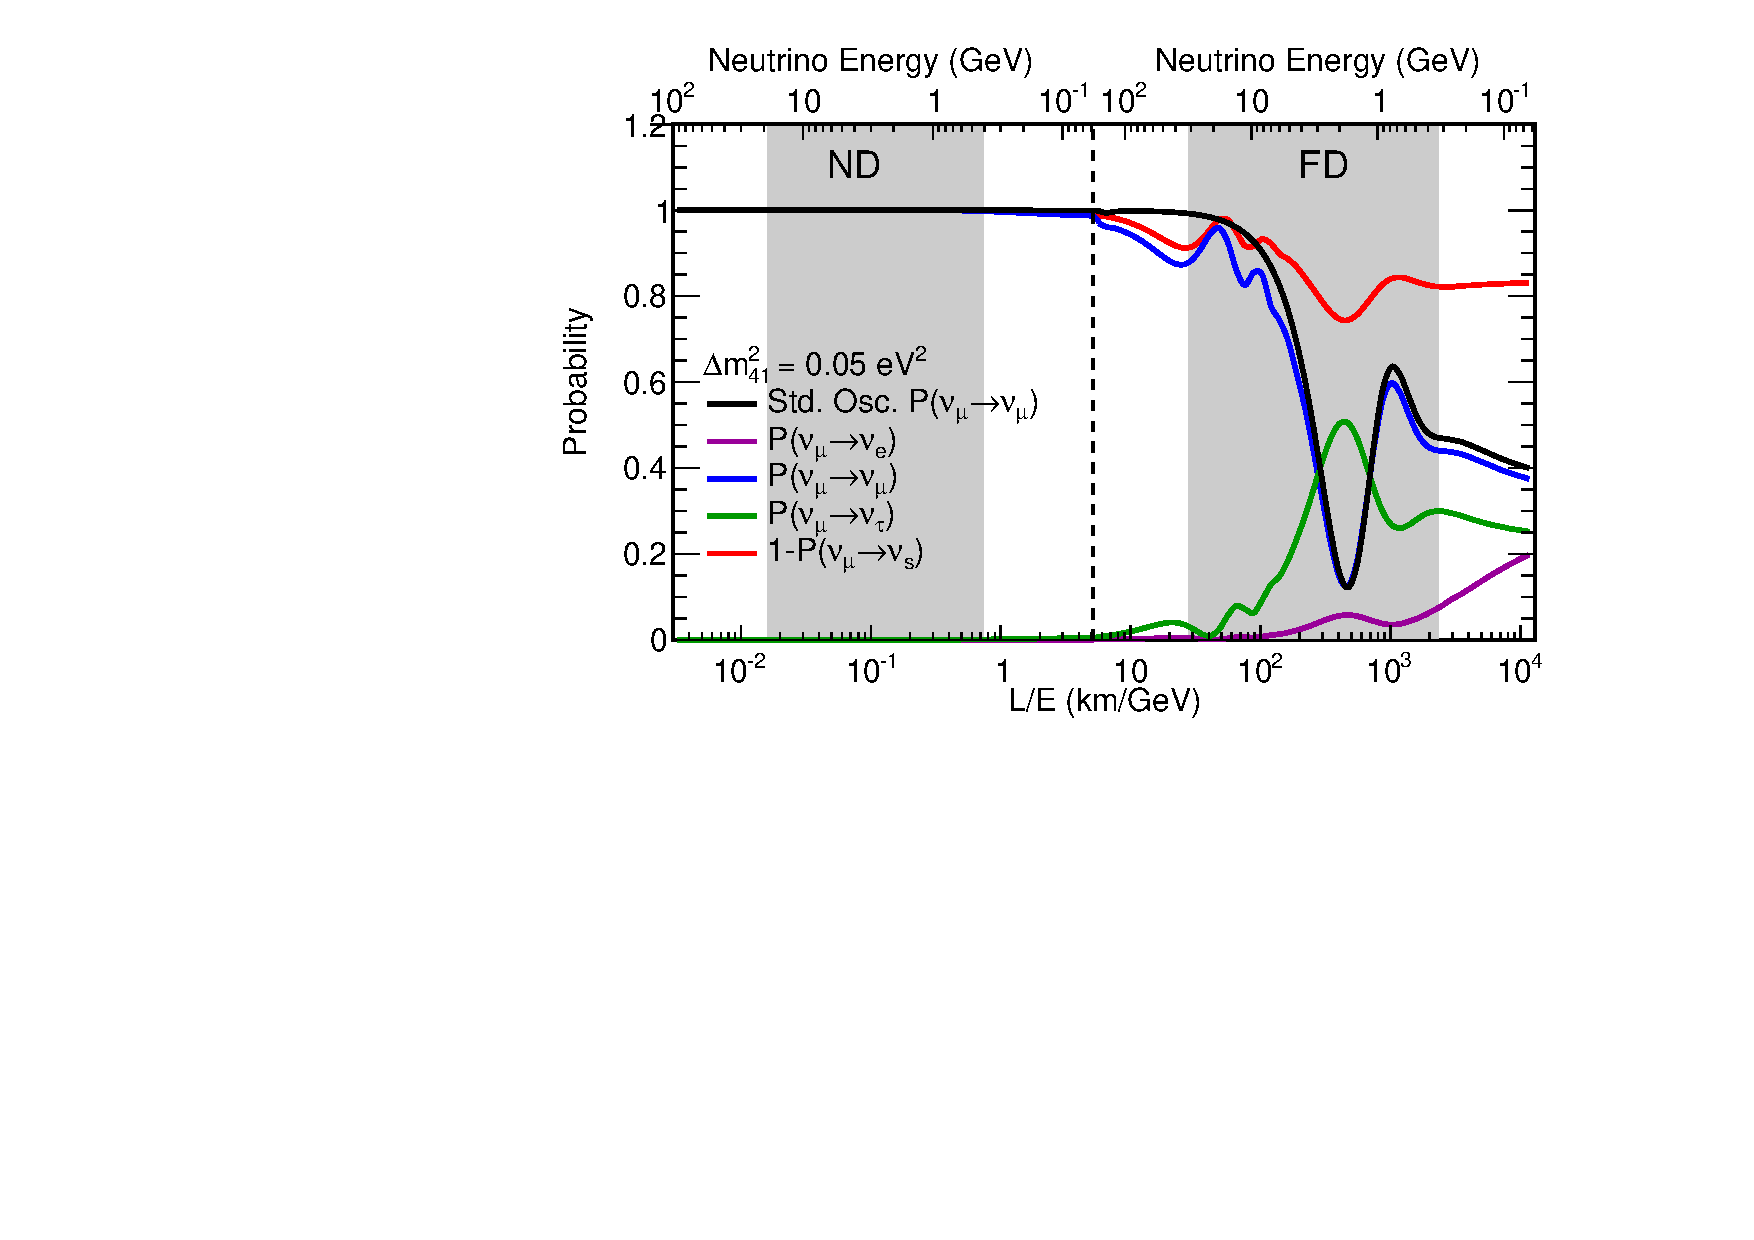
\includegraphics[width=0.49\textwidth]{DUNE_SterileSensi_dm0_05.pdf}
        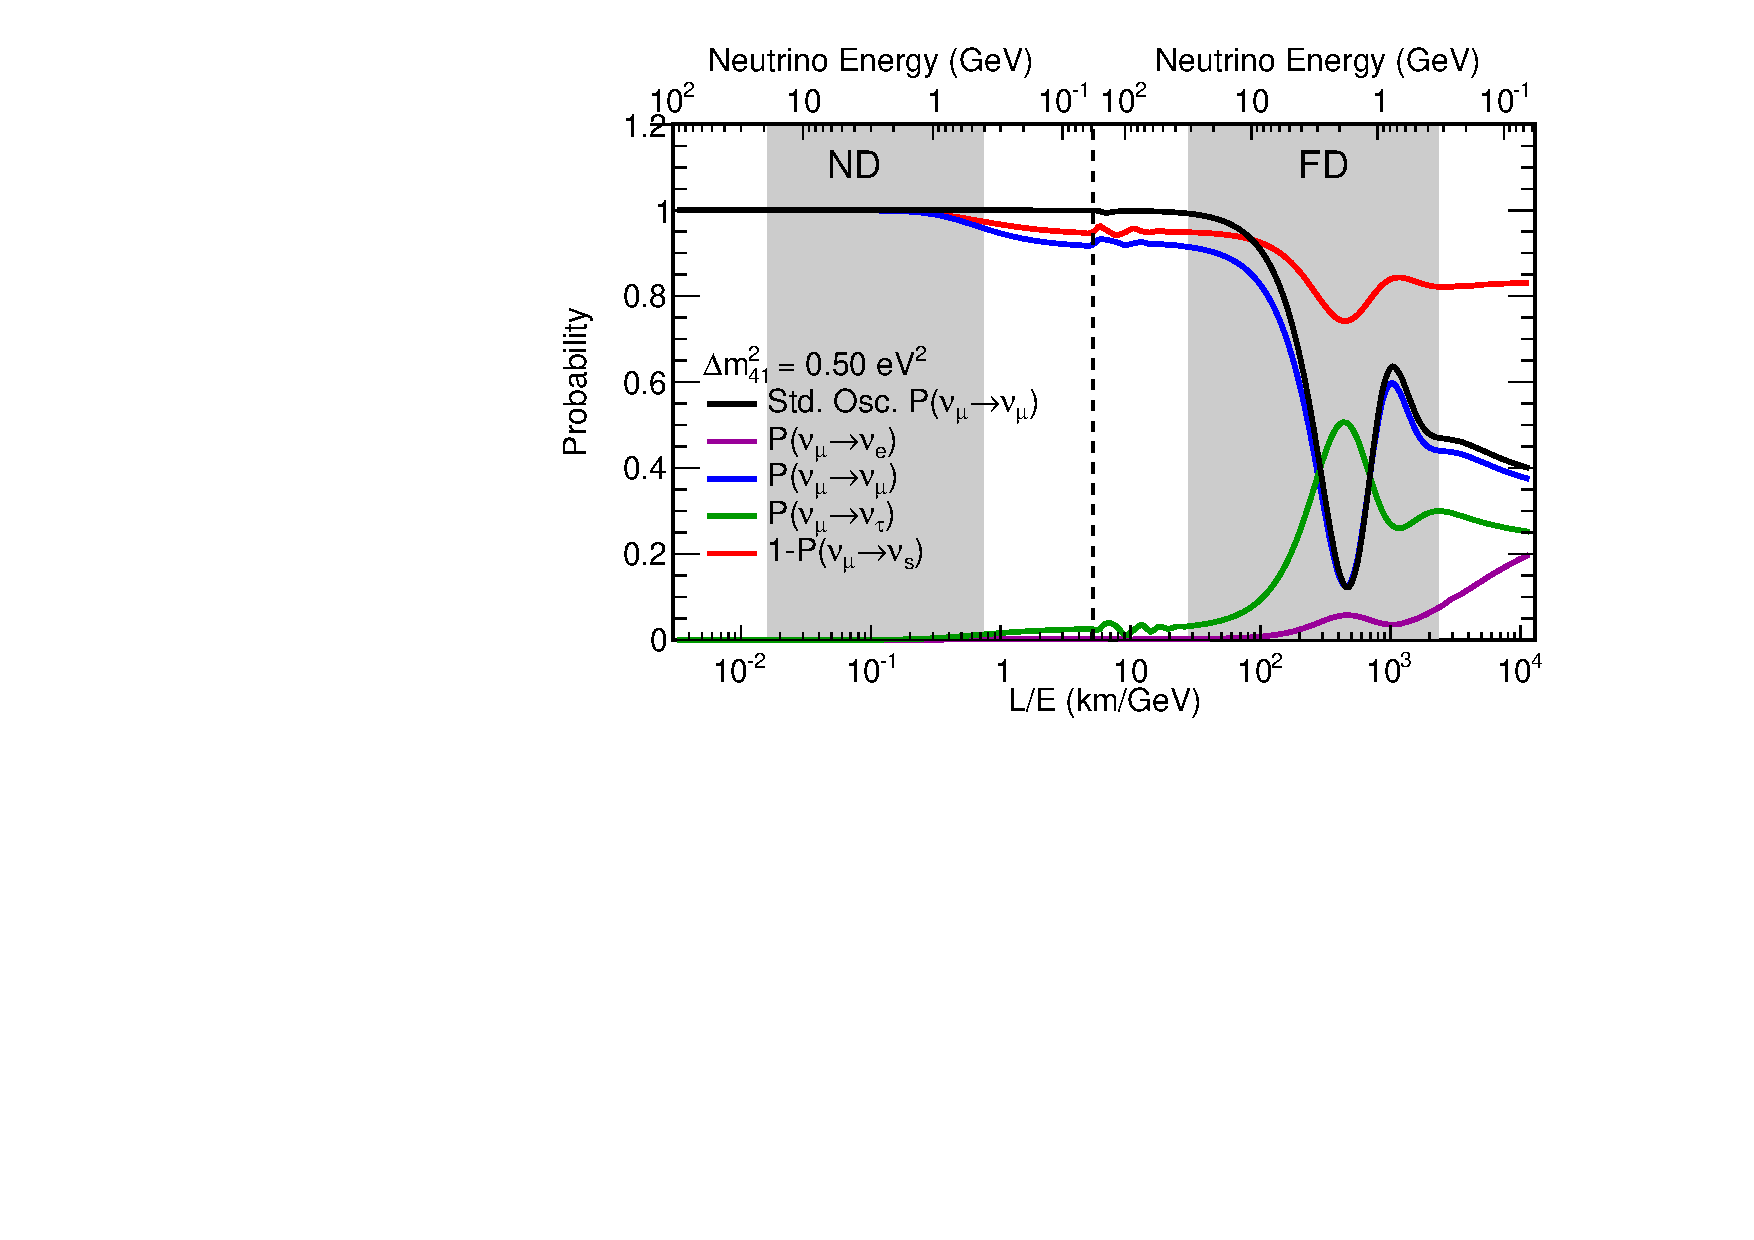
\includegraphics[width=0.49\textwidth]{DUNE_SterileSensi_dm0_5.pdf}
        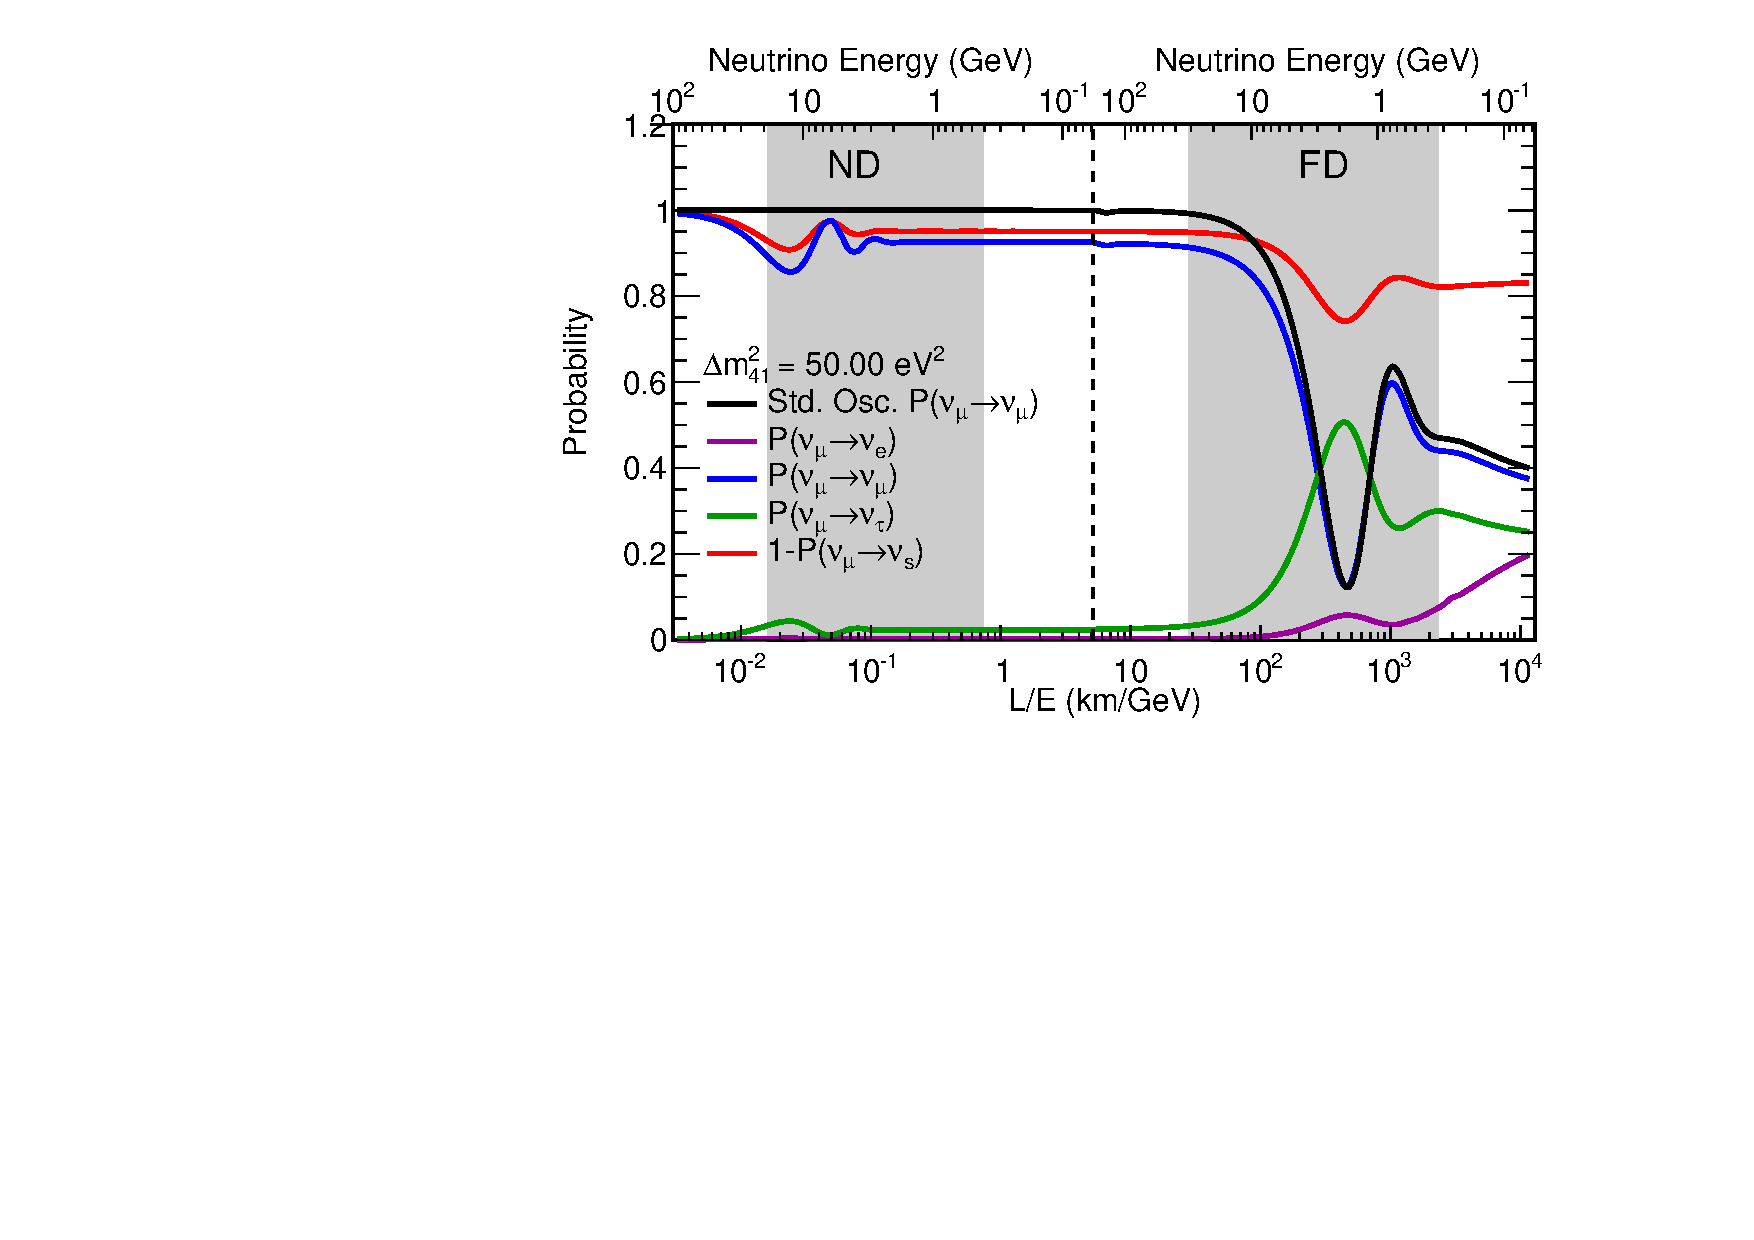
\includegraphics[width=0.49\textwidth]{DUNE_SterileSensi_dm50.pdf}
	\end{center}
\caption[Regions of $L/E$ probed by DUNE for %compared to 
3-flavor and 3+1-flavor $\nu$ oscillations]
{Regions of $L/E$ probed by the DUNE detector compared to 3-flavor and 3+1-flavor neutrino disappearance and appearance probabilities. The gray-shaded areas show the range of true neutrino energies probed by the \dword{nd} and \dword{fd}. The top axis shows true neutrino energy, increasing from right to left. The top-left plot shows the probabilities assuming mixing with one sterile neutrino with $\Delta m^2_{\rm{41}}=0.05$~eV$^2$, corresponding to the slow oscillations regime. The top-right plot assumes mixing with one sterile neutrino with $\Delta m^2_{\rm{41}}=0.5$~eV$^2$, corresponding to the intermediate oscillations regime. The bottom plot includes mixing with one sterile neutrino with $\Delta m^2_{\rm{41}}=50$~eV$^2$, corresponding to the rapid oscillations regime. As an example, the slow sterile oscillations cause visible distortions in the three-flavor \numu~survival probability (blue curve) for neutrino energies $\sim10$\,GeV, well above the three-flavor oscillation minimum.}
\label{fig:regimes}
\end{figure}


%%%%%%%%%%%%%%%%%%%%%%%%%
\subsection{Setup and Methods}
The simulation of the DUNE experimental setup was performed with the \dword{globes} software~\cite{Huber:2004ka,Huber:2007ji} using the same flux and equivalent detector definitions used by the three-neutrino flavor analysis presented in Section~\ref{sec:physics-lbnosc-simreco}. Specifically, the neutrino flux used assumes 120 GeV protons incident on the LBNF target, with $1.1\times 10^{21}$~\dword{pot} collected per year. A total exposure of 300~kton.MW.year is used in assessing DUNE's physics reach in probing the relevant sterile neutrino mixing parameter space.

The sterile neutrino effects have been implemented in  \dword{globes} via the existing plug-in for sterile neutrinos and \dword{nsi}~\cite{Joachim}. As described above, the \dword{nd} will play a very important role in the sensitivity to sterile neutrinos both directly, for rapid oscillations with $\Delta m_{41}^2 > 1$~eV$^2$ where the sterile oscillation matches the \dword{nd} baseline, and indirectly, at smaller values of $\Delta m_{41}^2$ where the \dword{nd} is crucial to reduce the systematics affecting the \dword{fd} to increase its sensitivity. To include these \dword{nd} effects in these studies, the latest \dword{globes} DUNE \dword{tdr} configuration files describing the detectors were modified by adding a \dword{nd} with correlated systematic errors with the \dword{fd}. As a first approximation, the \dword{nd} is assumed to be an identical scaled-down version of the TDR \dword{fd} where the same efficiencies, backgrounds and energy reconstruction as presented in Section~\ref{sec:physics-lbnosc-simreco} have been assumed, with detector properties the same as described in Section~\ref{sec:ndprops}. The systematic uncertainties originally defined in the \dword{globes} DUNE \dword{cdr} configuration already took into account the effect of the \dword{nd} constraint. Thus, since we are now explicitly simulating the \dword{nd}, larger uncertainties have been adopted but partially correlated between the different channels in the \dword{nd} and \dword{fd}, so that their impact is reduced by the combination of both data sets. The full list of systematic uncertainties considered and their values is summarized in a technical note~\cite{ref:dune-sterile-note}.

Finally, for oscillations observed at the \dword{nd}, the uncertainty on the production point of the neutrinos can play an important role. We have included an additional $20\%$ energy smearing, which produces a similar effect given the $L/E$ dependence of oscillations. We implemented this smearing in the \dword{nd} through multiplication of the migration matrices provided with the \dword{globes} files by an additional matrix with the $20\%$ energy smearing obtained by integrating the Gaussian
\begin{equation}
R^c(E,E')\equiv\frac{1}{\sigma(E)\sqrt{2\pi}}e^{-\frac{(E-E')^2}{2\sigma(E)}},
\label{R_mat}
\end{equation}
with $\sigma(E)=0.2 E$ in reconstructed energy $E'$.

%%%%%%%%%%%%%%%%%%%%%%%%%
\subsection{Results}
By default, \dword{globes} treats all systematic uncertainties included in the fit as normalization shifts. However, depending on the value of $\Delta m^2_{41}$, sterile mixing will induce shape distortions in the measured energy spectrum beyond simple normalization shifts. As a consequence, shape uncertainties are very relevant for sterile neutrino searches, particularly in regions of parameter space where the \dword{nd}, with virtually infinite statistics, has a dominant contribution. The correct inclusion of systematic uncertainties affecting the shape of the energy spectrum in the two-detector fit \dword{globes} framework used for this analysis posed technical and computational challenges beyond the scope of the study.
Therefore, for each limit plot, we present two limits bracketing the expected DUNE sensitivity limit, namely: the black limit line, a best-case scenario, where only normalization shifts are considered in a \dword{nd}+\dword{fd} fit, where the ND statistics and shape have the strongest impact; and the grey limit line, corresponding to a worst-case scenario where only the \dword{fd} is considered in the fit, together with a rate constraint from the \dword{nd}. 

Studying the sensitivity to $\theta_{14}$, the dominant channels are those regarding $\nu_e$ disappearance. Therefore, only the $\nu_e$ \dword{cc} sample is analyzed and the channels for \dword{nc} and $\nu_{\mu}$ \dword{cc} disappearance are not taken into account, as they do not influence greatly the sensitivity and they slow down the simulations. The sensitivity at the 90\% \dword{cl}, taking into account the systematics mentioned above, is shown in Figure~\ref{fig:th_14+th_24}, along with a comparison to current constraints.

For the $\theta_{24}$ mixing angle, we analyze the $\nu_{\mu}$ \dword{cc} disappearance and the \dword{nc} samples, which are the main contributors to the sensitivity. 
The results are shown in Figure~\ref{fig:th_14+th_24}, along with comparisons with present constraints.

\begin{dunefigure}[Sensitivities to $\theta_{14}$ from $\nu_e$ CC samples, and to $\theta_{24}$ using $\nu_\mu$ CC and NC samples] %, from the \dword{nd} and \dword{fd} in both cases.]
{fig:th_14+th_24}
{The left-hand plot shows the DUNE sensitivities to $\theta_{14}$ from the $\nu_e$ \dword{cc} samples at the \dword{nd} and \dword{fd}, along with a comparison with the combined reactor result from Daya Bay and Bugey-3. The right-hand plot displays sensitivities to $\theta_{24}$ using the $\nu_\mu$ \dword{cc} and \dword{nc} samples at both detectors, along with a comparison with previous and existing experiments. In both cases, regions to the right of the contours are excluded.}
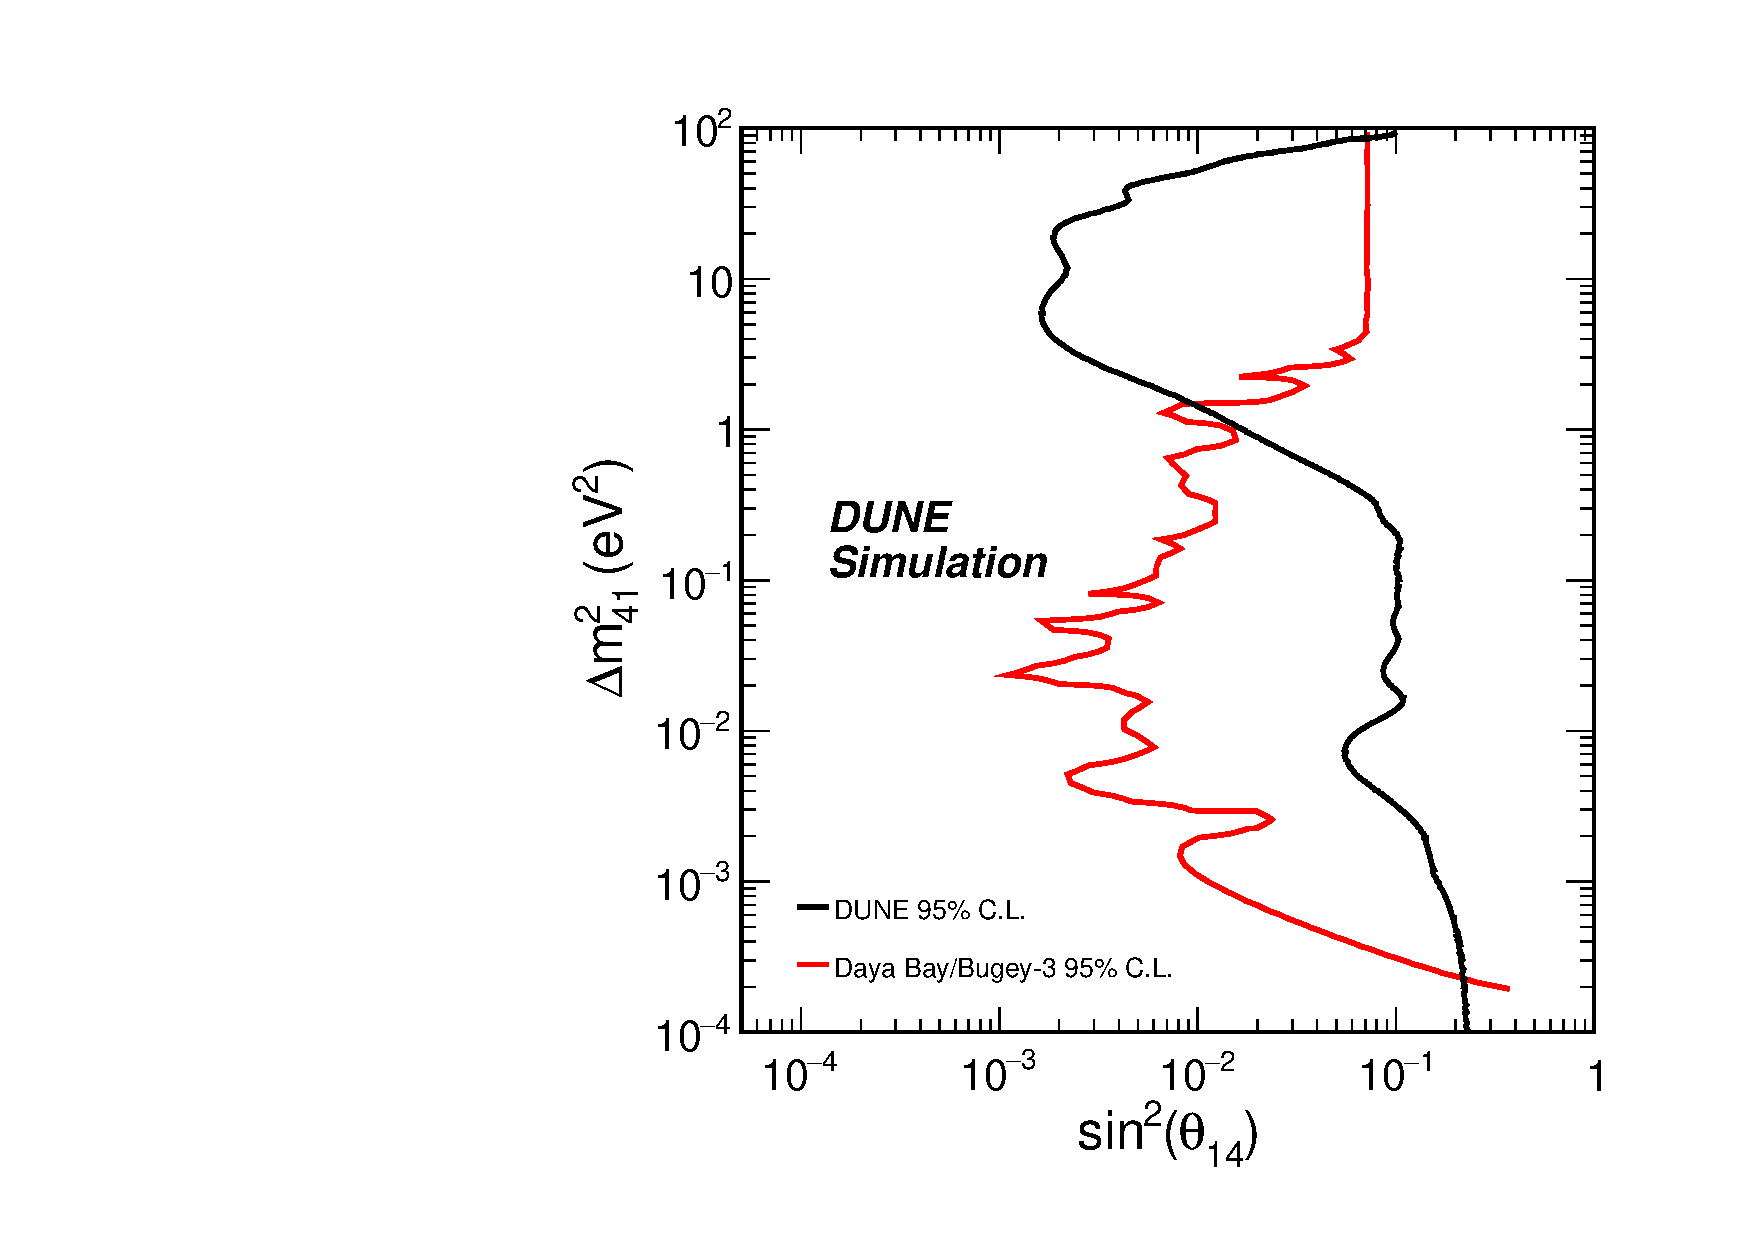
\includegraphics[width=0.48\columnwidth]{MultiPlots_DUNE_th14_prelim}
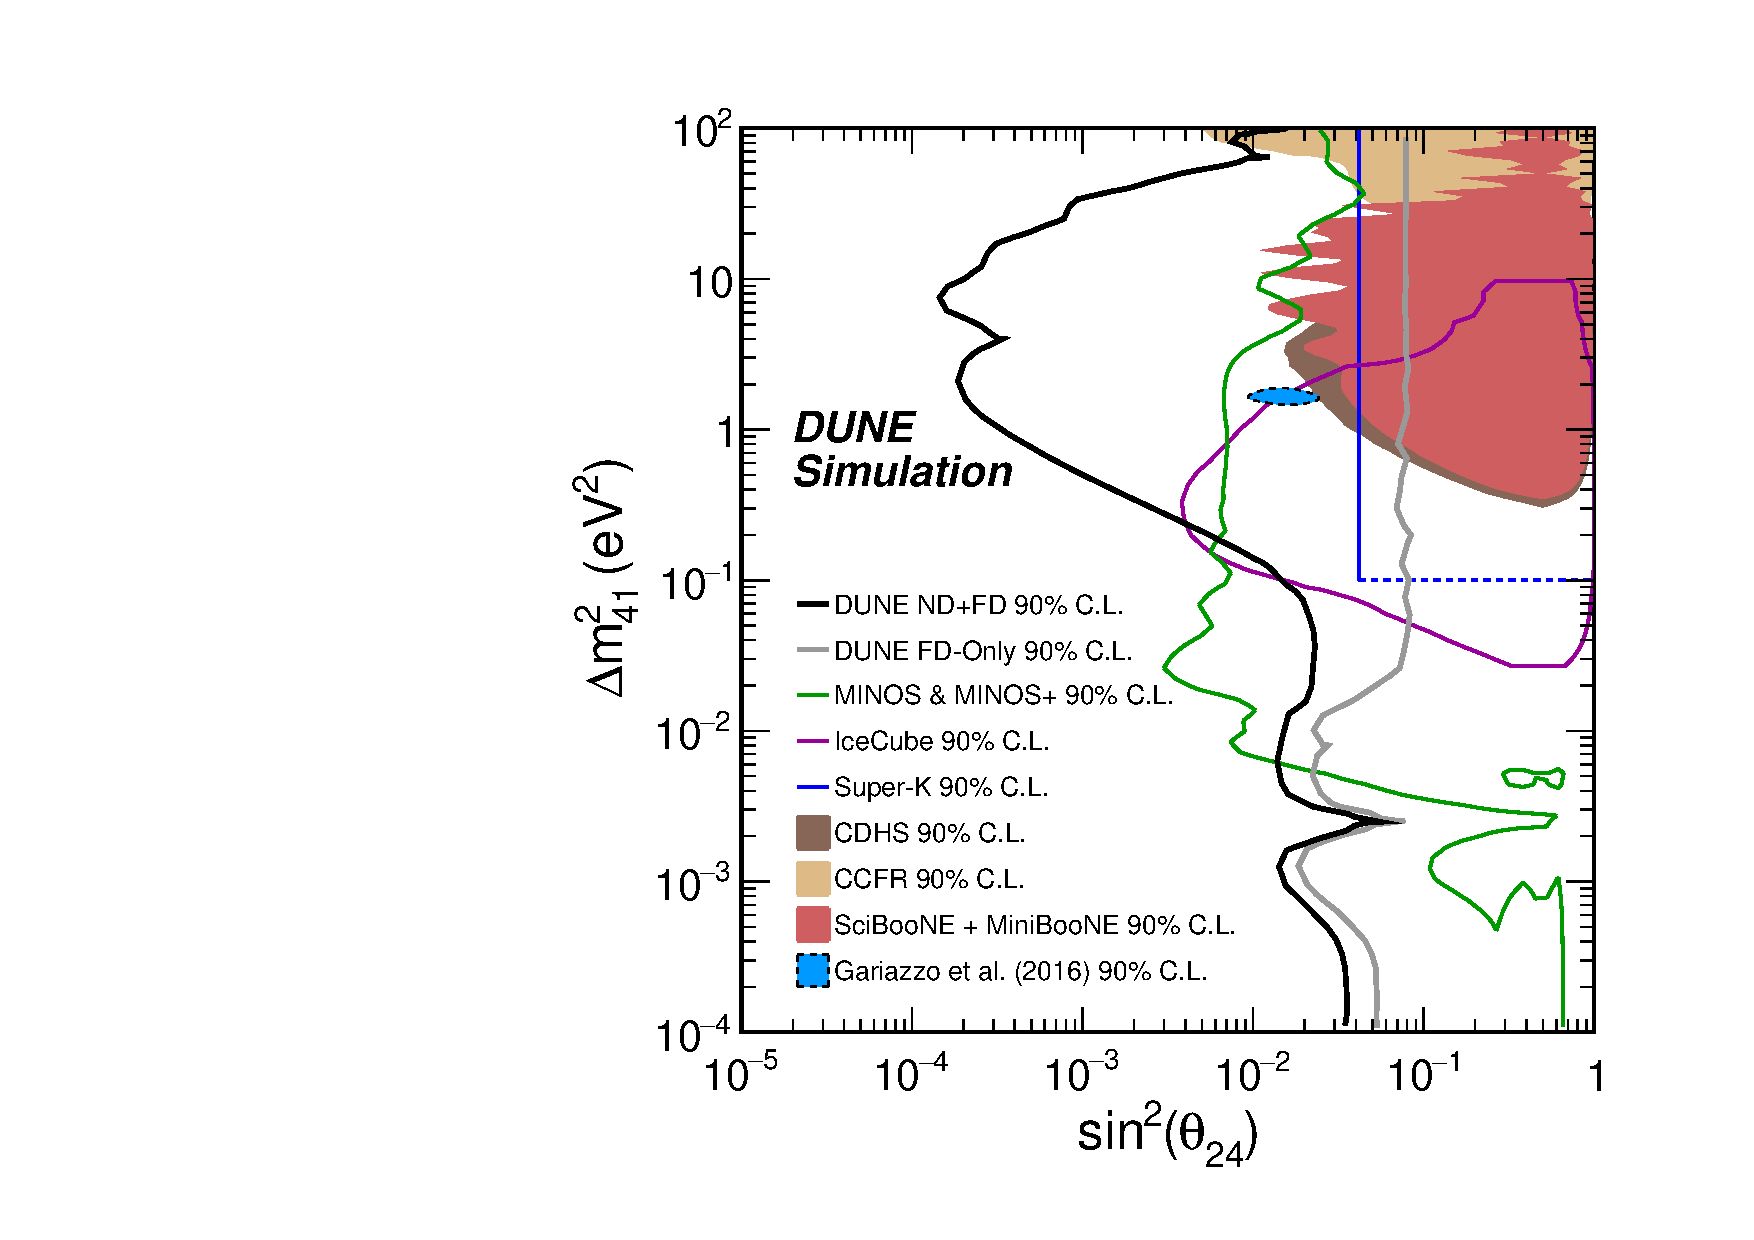
\includegraphics[width=0.48\columnwidth]{MultiPlots_DUNE_MINOS_IceCube_globAppF_prelim.pdf}
\end{dunefigure}


In the case of the $\theta_{34}$ mixing angle, we look for disappearance in the \dword{nc} sample, the only contributor to this sensitivity. The results are shown in Figure~\ref{fig:th_34}. Further, a comparison with previous experiments sensitive to \numu, \nutau~mixing with large mass-squared splitting is possible by considering an effective mixing angle $\theta_{\mu\tau}$, such that $\sin^2{2\theta_{\mu\tau}}\equiv 4|U_{\tau4}|^2|U_{\mu 4}|^2=\cos^4\theta_{14}\sin^22\theta_{24}\sin^2\theta_{34}$, and assuming conservatively that $\cos^4\theta_{14}=1$, and $\sin^22\theta_{24}=1$. This comparison with previous experiments is also shown in Figure~\ref{fig:th_34}.
The sensitivity to $\theta_{34}$ is largely independent of 
$\Delta m^2_{41}$, since the term with $\sin^2\theta_{34}$ in the expression describing $P(\nu_{\mu} \rightarrow \nu_s)$ Eq.~\ref{eq:numu_nus}, depends solely on the $\Delta m^2_{31}$ mass splitting.

\begin{dunefigure}[Sensitivity to $\theta_{34}$ using the NC samples at the ND and FD] {fig:th_34} 
{DUNE sensitivity to $\theta_{34}$ using the \dword{nc} samples at the \dword{nd} and \dword{fd} compared to previous and existing experiments. Regions to the right of the contour are excluded.}
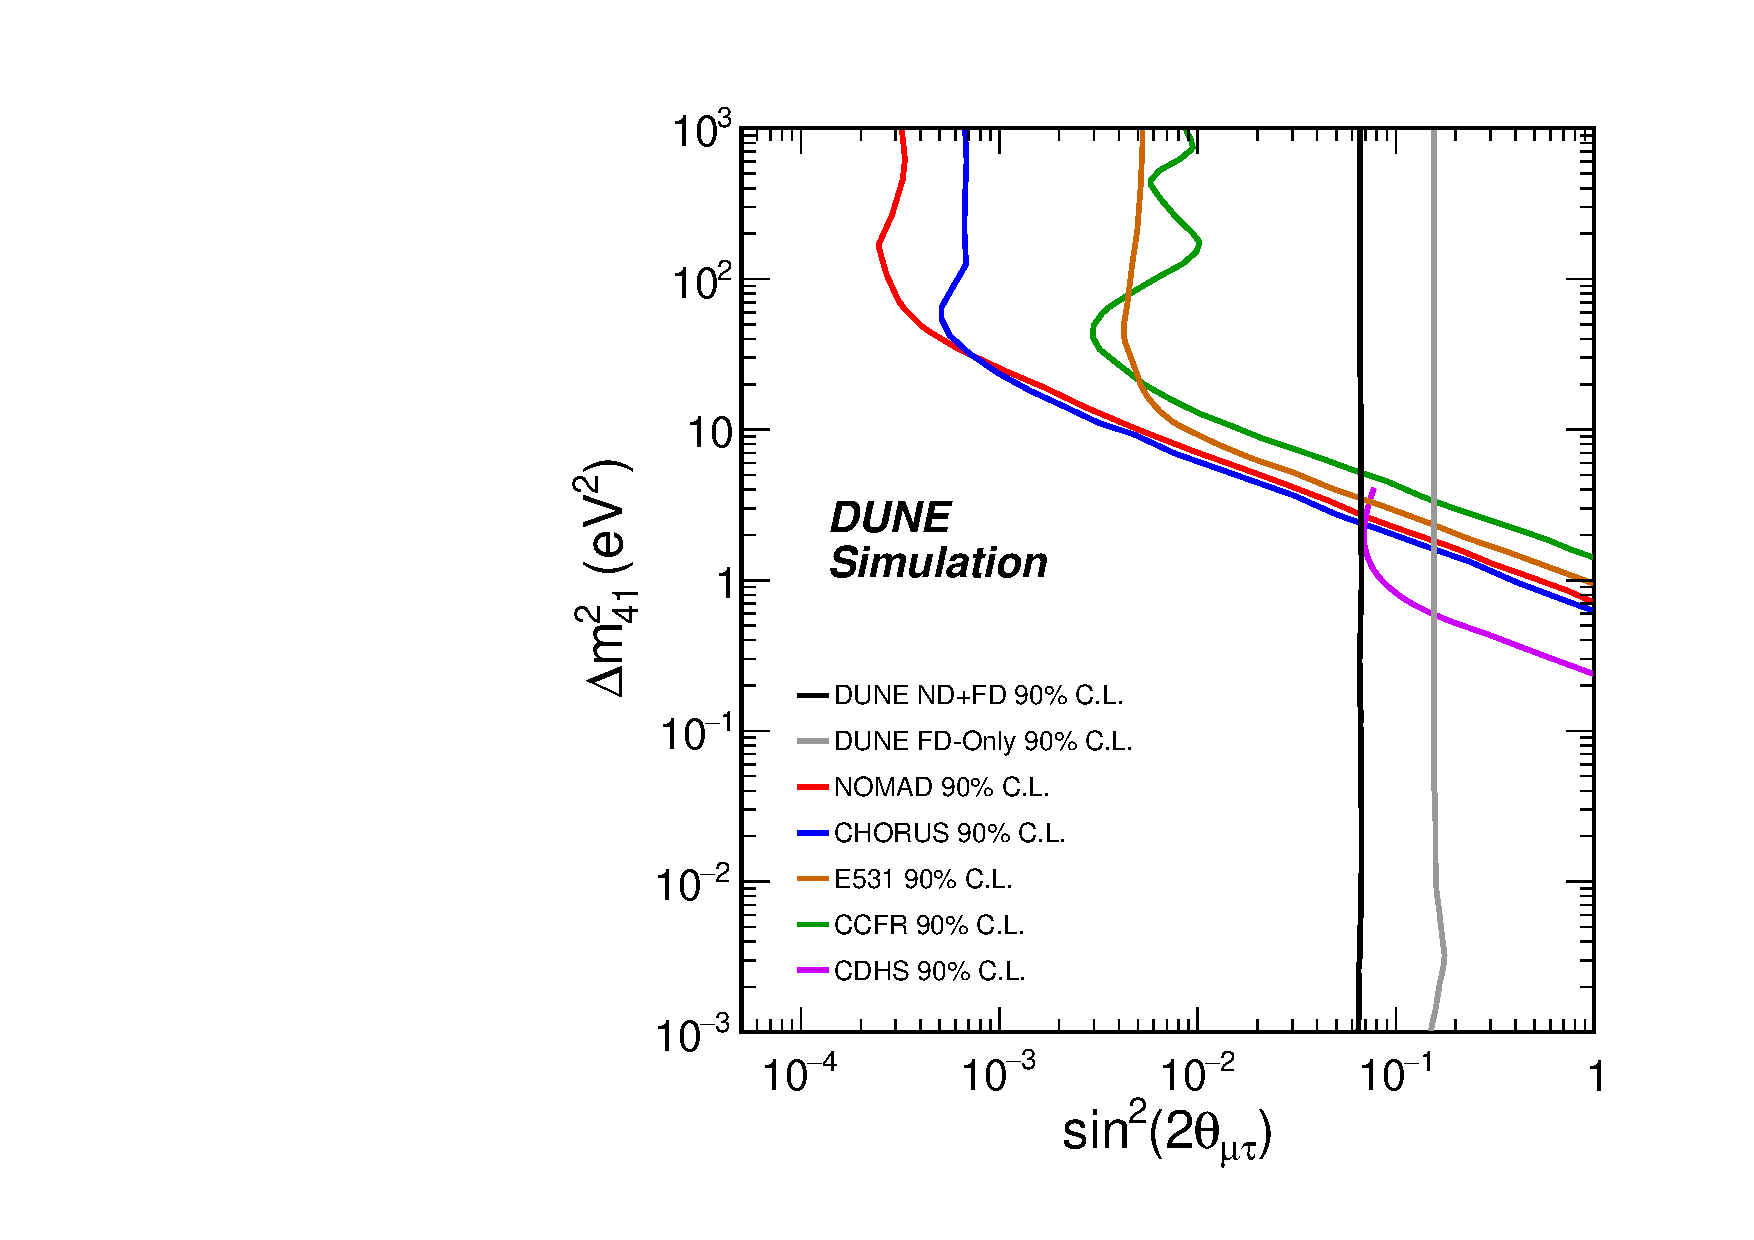
\includegraphics[width=0.48\columnwidth]{MultiPlots_DUNE_th34_prelim1}
\end{dunefigure}



Another quantitative comparison of our results for $\theta_{24}$ and $\theta_{34}$ with existing constraints can be made for projected upper limits on the sterile mixing angles assuming no evidence for sterile oscillations is found, and picking the value of  $\Delta m^2_{41} = 0.5$~eV$^2$ corresponding to the simpler counting experiment regime. For the $3+1$ model, upper limits of $\theta_{24}$\,$<$\,$1.8^{\circ}(15.1^{\circ})$ and $\theta_{34}$\,$<$\,$15.0^{\circ}(25.5^{\circ})$ are obtained at the 90\% \dword{cl} from the presented best(worst)-case scenario DUNE sensitivities. If expressed in terms of the relevant matrix elements
\begin{align}
\begin{split}
|U_{\mu4}|^2 =&\,\,\cos^2\theta_{14}\sin^2\theta_{24} \\
|U_{\tau4}|^2= & \,\,\cos^2\theta_{14}\cos^2\theta_{24}\sin^2\theta_{34},
\end{split}
\label{eq:DisapToApp}
\end{align}
these limits become $|U_{\mu4}|^{2}$\,$<$\,0.001(0.068) and $|U_{\tau4}|^{2}$\,$<$\,0.067(0.186) at the 90\% \dword{cl}, where we conservatively assume $\cos^2\theta_{14}$\,=\,1 in both cases, and additionally $\cos^2\theta_{24}$\,=\,1 in the second case.
\begin{dunetable}
[Projected 90\% \dword{cl} upper limits on sterile mixing angles and matrix elements]
{c c c c c}
{tab:limits}
{The projected DUNE 90\% \dword{cl} upper limits on sterile mixing angles and matrix elements compared to the equivalent 90\% \dword{cl} upper limits from \nova~\cite{ref:novasterile}, MINOS/MINOS+~\cite{Adamson:2017uda}, \superk~\cite{ref:superksterile}, IceCube~\cite{ref:IceCube}, and IceCube-DeepCore~\cite{ref:DeepCore}. The limits are shown for $\Delta m^2_{41} = 0.5$~eV$^2$ for all experiments, except for IceCube-DeepCore, where the results are reported for $\Delta m^2_{41} = 1.0$~eV$^2$.}
& $\theta_{24}$ & $\theta_{34}$ & $|U_{\mu4}|^2$ &  $|U_{\tau4}|^2$  \\ \toprowrule
DUNE Best-Case  & $1.8^{\circ}$ & $15.0^{\circ}$ & 0.001 & 0.067  \\ \colhline
DUNE Worst-Case  & $15.1^{\circ}$ & $25.5^{\circ}$ & 0.068 & 0.186  \\ \colhline
NOvA  & $20.8^{\circ}$ & $31.2^{\circ}$ & 0.126 & 0.268  \\ \colhline
MINOS/MINOS+ & $4.4^{\circ}$ & $23.6^{\circ}$ & 0.006 & 0.16  \\ \colhline
\superk & $11.7^{\circ}$ & $25.1^{\circ}$ & 0.041 & 0.18  \\ \colhline
IceCube & $4.1^{\circ}$ & \-- & 0.005 & \--   \\ \colhline 
IceCube-DeepCore & $19.4^{\circ}$ & $22.8^{\circ}$ & 0.11 & 0.15 \\
\end{dunetable}  
  
Finally, sensitivity to the $\theta_{\mu e}$ effective mixing angle, defined above as $\sin^2{2\theta_{\mu e}}\equiv 4|U_{e4}|^2|U_{\mu 4}|^2=\sin^22\theta_{14}\sin^2\theta_{24}$, is shown in Figure~\ref{fig:th_me}, which also displays a comparison with the allowed regions from \dword{lsnd} and MiniBooNE, as well as with present constraints and projected constraints from the \fnal \dword{sbn} program.

Further, to illustrate that DUNE would not be limited to constraining active-sterile neutrino mixing, we have produced a discovery potential plot, for a scenario with one sterile neutrino governed by the \dword{lsnd} best-fit parameters: $\left(\Delta m_{14}^2= 1.2\;\text{eV}^2;\,\,\sin^2{2\theta_{\mu e}}=0.003\right)$~\cite{LSNDSterile}. 
A small 90\% \dword{cl} allowed region, shown in Figure~\ref{fig:th_me}, is obtained, which can be compared with the \dword{lsnd} allowed region in the same figure. 
\begin{dunefigure}
[Sensitivity to $\theta_{\mu e}$ from  (dis)appearance samples and discovery potential at \dword{lsnd} best fit]
{fig:th_me}
{DUNE sensitivities to $\theta_{\mu e}$ from the appearance and disappearance samples at the \dword{nd} and \dword{fd} is shown on the left-hand plot, along with a comparison with previous existing experiments and the sensitivity from the future \dword{sbn} program. Regions to the right of the DUNE contours are excluded. The right-hand plot displays the discovery potential assuming $\theta_{\mu e}$ and $\Delta m_{41}^2$ set at the best-fit point determined by \dword{lsnd}~\cite{LSNDSterile} for the best-case scenario referenced in the text.}
$\vcenter{\hbox{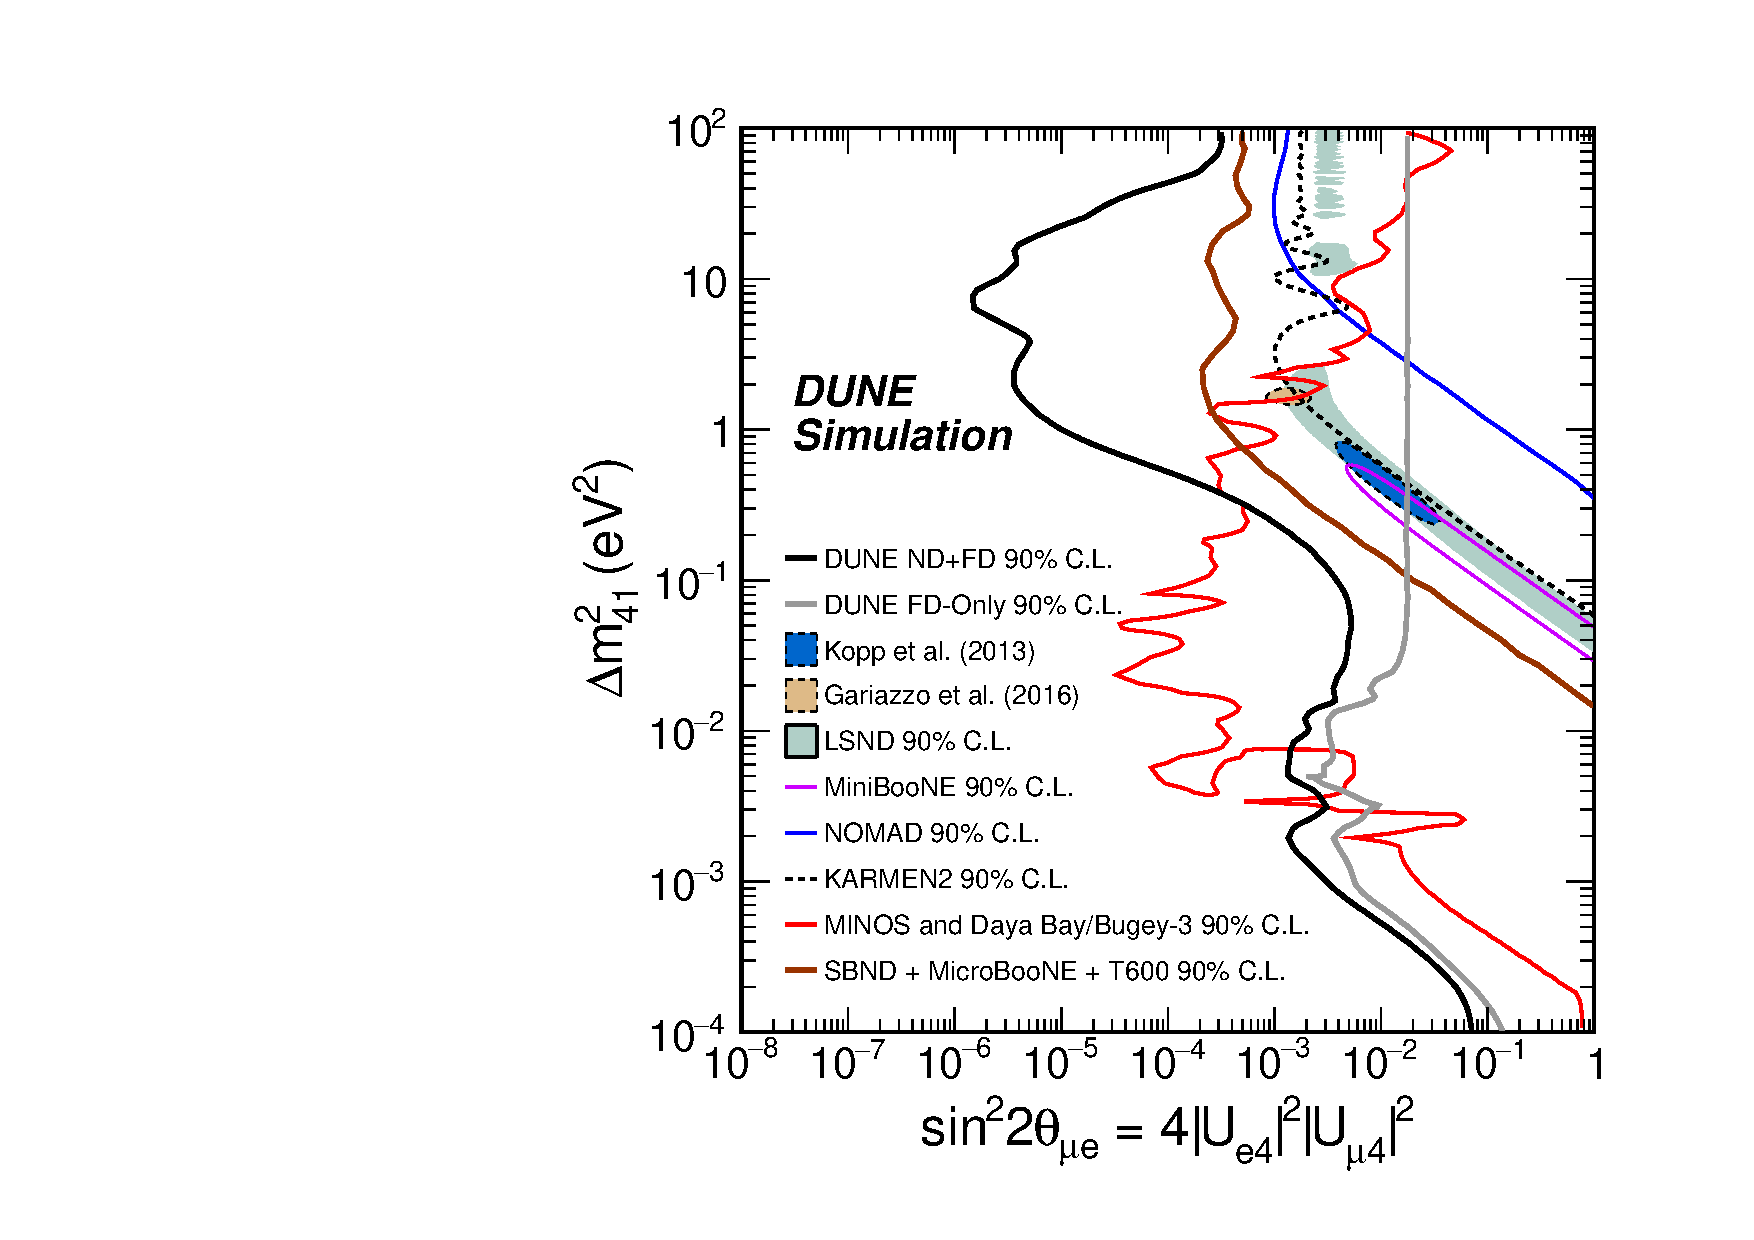
\includegraphics[width=0.48\columnwidth]{ComboLimit90_dune_sbn.pdf}}}$
$\vcenter{\hbox{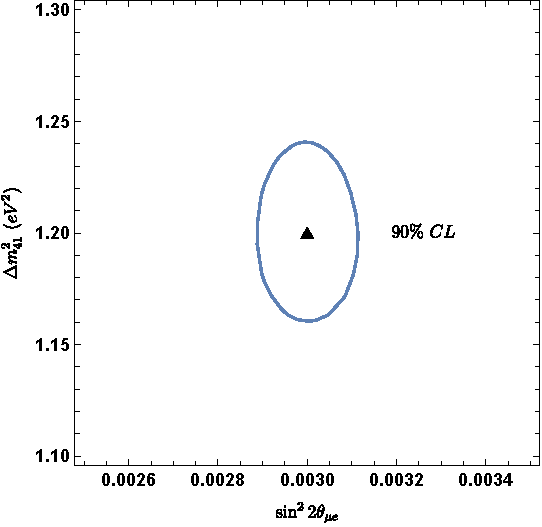
\includegraphics[width=0.42\columnwidth]{Dis_Pot_tme.pdf}}}$
\end{dunefigure}



The physics reach plots shown above illustrate the excellent potential of DUNE to discover or constrain mixing with sterile neutrinos. Notably, in the case of sterile-mediated \numu~to \nue~transitions, DUNE can place very competitive constraints on its own, without requiring a combination with reactor experiments. 

%\subsection{Discussion of potential enhancements from hardware improvements}
These studies show compelling motivation for DUNE to deploy a highly-capable \dword{nd}  given its high potential for discovery or constraining of new physics, including mixing with sterile neutrino species. These capabilities can be further improved by a high-precision muon monitor system for the LBNF beam, which would provide an independent constraint on the neutrino flux through measurements of the associated muon flux, not susceptible to mixing with sterile neutrinos.


%%%%%%%%%%%%%%%%%%%%%%%%%%%%%%%%%%%%%%%%
%\section{Searches for Non-Standard Interactions, Non-Unitarity, and \dword{cpt} Symmetry Violation}
%%%%%%%%%%%%%%%%%%%%%%%%%


%%%%%%%%%%%%%%%%%%%%%%%%%
\section{Non-Unitarity of the Neutrino Mixing Matrix}
\label{sec:nonUnitarity}
%{\bf Authors: Fernandez-Martinez, Forero, Miranda, Tórtola
%\vspace{0.5cm}
A generic characteristic of most models explaining the neutrino mass
pattern is the presence of heavy neutrino states, beyond the
three light states of the \dword{sm}  of particle
physics~\cite{Minkowski:1977sc,Mohapatra:1979ia,Yanagida:1979as,GellMann:1980vs}. This implies a deviation from unitarity of the $3\times3$ \dword{pmns} matrix, which can be particularly sizable %the lower the mass of the extra states are
as the mass of the extra states becomes lower~\cite{Lee:1977tib,Schechter:1980gr,Mohapatra:1986bd,Akhmedov:1995vm,Akhmedov:1995ip,Malinsky:2005bi}.
For values of non-unitarity parameter deviations of order $10^{-2}$, this would decrease the expected reach of DUNE to the standard parameters, although stronger bounds existing from charged leptons would be able to restore its expected performance~\cite{Blennow:2016jkn,Escrihuela:2016ube}.

A generic characteristic of most models explaining the neutrino mass
pattern is the presence of heavy neutrino states, additional to the
three light states of the \dword{sm}  of particle
physics~\cite{Mohapatra:1998rq,Valle:2015pba,Fukugita:2003en}. These
types of models will imply that the $3 \times 3$ \dword{pmns} matrix is not unitary due to the mixing with the additional states.  Besides the type-I seesaw
mechanism~\cite{GellMann:1980vs,Yanagida:1979as,Mohapatra:1979ia,Schechter:1980gr},
different low-scale seesaw models include right-handed neutrinos that are relatively not-so-heavy~\cite{Mohapatra:1986bd} and perhaps detectable at collider experiments.

These additional heavy leptons would mix with the light neutrino states and, as a result, the complete unitary mixing matrix would be a squared $n \times n$ matrix, with $n$ the total number of neutrino
states. As a result, the usual $3 \times 3$ \dword{pmns} matrix, which we dub $N$ to stress its non-standard nature, will be
non-unitary. One possible general way to parameterize these unitarity deviations in $N$ is through a triangular matrix~\cite{Escrihuela:2015wra}\footnote{For a similar parameterization corresponding to a $(3+1)$ and a $(3+3)$-dimensional mixing matrix,  see Refs.~\cite{Xing:2007zj,Xing:2011ur}}
%%
 \begin{equation}
  N = 
 \left\lgroup
 \begin{array}{ccc} 
 1-\alpha_{ee} & 0 & 0 \\
 \alpha_{\mu e} & 1-\alpha_{\mu \mu} & 0 \\
  \alpha_{\tau e} & \alpha_{\tau \mu} & 1-\alpha_{\tau \tau}
 \end{array}
 \right \rgroup U \,,
 \label{eq:triangular}
 \end{equation}
 % 
with $U$ a unitary matrix that tends to the usual \dword{pmns} matrix when the non-unitary parameters $\alpha_{ij} \rightarrow 0$\footnote{The original parameterization in Ref.~\cite{Escrihuela:2015wra} uses $\alpha_{ii}$ instead of $\alpha_{\beta\gamma}$. The equivalence between the two notations is as follows: $\alpha_{ii} = 1-\alpha_{\beta\beta}$ and $\alpha_{ij} = \alpha_{\beta\gamma}$.} .
%
The triangular matrix in this equation accounts for the non-unitarity of the $3 \times 3$ matrix for any number of extra neutrino species. This parametrization has been shown to be particularly well-suited for oscillation searches~\cite{Escrihuela:2015wra,Blennow:2016jkn} since, compared to other alternatives, it minimizes the departures of its unitary component $U$ from the mixing angles that are directly measured in neutrino oscillation experiments when unitarity is assumed.

The phenomenological implications of a non-unitary leptonic mixing matrix have been extensively studied in flavor and electroweak precision observables as well as in the neutrino oscillation phenomenon~\cite{Shrock:1980vy,Schechter:1980gr,Shrock:1980ct,Shrock:1981wq,Langacker:1988ur,Bilenky:1992wv,Nardi:1994iv,Tommasini:1995ii,Antusch:2006vwa,FernandezMartinez:2007ms,Antusch:2008tz,Biggio:2008in,Antusch:2009pm,Forero:2011pc,Alonso:2012ji,Antusch:2014woa,Abada:2015trh,Fernandez-Martinez:2015hxa,Escrihuela:2015wra,Parke:2015goa,Miranda:2016wdr,Fong:2016yyh,Escrihuela:2016ube}. For recent global fits to all flavor and electroweak precision data summarizing present bounds on non-unitarity see Refs.~\cite{Antusch:2014woa,Fernandez-Martinez:2016lgt}. 



%%%%%%%%%%%%%%%%%%%%%
\begin{dunetable}
[Expected 90\%~CL constraints on the non-unitarity parameters $\alpha$]
{|c|c|}
{tab:bounds}
{Expected $90\%$~\dword{cl} constraints on the non-unitarity parameters $\alpha$ from DUNE.}
{\bf Parameter} & {\bf Constraint} \\ \toprowrule
$\alpha_{ee}$ & $0.3$   \\ \colhline
$\alpha_{\mu\mu}$ & $0.2$ \\ \colhline
$\alpha_{\tau\tau}$ & $0.8$ \\ \colhline
$\alpha_{\mu e}$ & $0.04$ \\ \colhline
$\alpha_{\tau e}$ & $0.7$ \\ \colhline
$\alpha_{\tau\mu}$ & $0.2$ \\
\end{dunetable}
%%%%%%%%%%%%%%%%%%%%%

\subsection{NU constraints from DUNE}
Recent studies have shown that DUNE can constrain the non-unitarity parameters~\cite{Blennow:2016jkn, Escrihuela:2016ube}. The summary of the $90 \%$~\dword{cl}  bounds on the different $\alpha_{ij}$ elements profiled over all other parameters is given in Table~\ref{tab:bounds}. 
These bounds are comparable with other constraints from present oscillation experiments, although they are not competitive with those obtained from flavor and electroweak precision data.
For this analysis, and %the ones that will be 
those presented below, we have used the \dword{globes} software~\cite{Huber:2004ka,Huber:2007ji} with the DUNE \dword{cdr} configuration presented in Ref.~\cite{Alion:2016uaj}, and assuming a data exposure of 300~kton.MW.year. The standard (unitary) oscillation parameters have also been treated as in~\cite{Alion:2016uaj}. The unitarity deviations have been included both by an independent code (used to obtain the results shown in Ref.~\cite{Escrihuela:2016ube}) and via the MonteCUBES~\cite{Blennow:2009pk} plug-in to cross validate our results.

\subsection{NU impact on DUNE standard searches}
Conversely, the presence of non-unitarity may affect the determination of the
Dirac \dword{cp}-violating phase $\delta_{CP}$ in long-baseline experiments~\cite{Miranda:2016wdr,Fernandez-Martinez:2016lgt,Escrihuela:2016ube}.
Indeed, when allowing for unitarity deviations, the expected \dword{cp} discovery potential for DUNE could be significantly reduced.
However, the situation is alleviated when a combined analysis with the constraints on non-unitarity from other experiments is considered. This is illustrated in Figure~\ref{fig:CPsens}. In the left panel, the discovery potential for \dword{cpv} is computed when the non-unitarity parameters introduced in Eq.~(\ref{eq:triangular}) are allowed in the fit. While for the Asimov data all $\alpha_{ij}=0$, the non-unitary parameters are allowed to vary in the fit with $1 \sigma$ priors of $10^{-1}$, $10^{-2}$ and $10^{-3}$ for the dotted green, dashed blue and solid black lines respectively. For the dot-dashed red line no prior information on the non-unitarity parameters has been assumed. As can be observed, without additional priors on the non-unitarity parameters, the capabilities of DUNE to discover \dword{cpv} from $\delta_{CP}$ would be seriously compromised~\cite{Escrihuela:2016ube}. However, with priors of order $10^{-2}$ matching the present constraints from other neutrino oscillation experiments~\cite{Escrihuela:2016ube,Blennow:2016jkn}, the standard sensitivity is almost recovered. If the more stringent priors of order $10^{-3}$ stemming from flavor and electroweak precision observables are added~\cite{Antusch:2014woa,Fernandez-Martinez:2016lgt}, the standard sensitivity is obtained.   

The right panel of Figure~\ref{fig:CPsens} concentrates on the impact of the phase of the element $\alpha_{\mu e}$ in the discovery potential of \dword{cpv} from $\delta_{CP}$, since this element has a very important impact in the $\nu_e$ appearance channel. In this plot the modulus of $\alpha_{ee}$, $\alpha_{\mu \mu}$ and $\alpha_{\mu e}$ have been fixed to $10^{-1}$, $10^{-2}$, $10^{-3}$ and 0 for the dot-dashed red, dotted green, dashed blue and solid black lines respectively. All other non-unitarity parameters have been set to zero and the phase of $\alpha_{\mu e}$ has been allowed to vary both in the fit and in the Asimov data, showing the most conservative curve obtained. As for the right panel, it can be seen that a strong deterioration of the \dword{cp} discovery potential could be induced by the phase of $\alpha_{\mu e}$ (see Ref.~\cite{Escrihuela:2016ube}). However, for unitarity deviations of order $10^{-2}$, as required by present neutrino oscillation data constraints, the effect is not too significant in the range of $\delta_{CP}$ for which a $3 \sigma$ exclusion of \dword{cp} conservation would be possible and it becomes negligible if the stronger $10^{-3}$ constraints from flavor and electroweak precision data are taken into account.  

Similarly, the presence of non-unitarity worsens degeneracies involving $\theta_{23}$, making the determination of the octant or even its maximality challenging.
This situation is shown in Figure~\ref{fig:octant} where an input value of $\theta_{23} = 42.3^\circ$ was assumed. As can be seen, the fit in presence of non-unitarity (solid lines) introduces degeneracies for the wrong octant and even for maximal mixing~\cite{Blennow:2016jkn}. However, these degeneracies are solved upon the inclusion of present priors on the non-unitarity parameters from other oscillation data (dashed lines) and a clean determination of the standard oscillation parameters following DUNE expectations is again recovered.   

\begin{dunefigure}
[Impact of non-unitarity on the CPV discovery potential]
{fig:CPsens}
{The impact of non-unitarity on the DUNE \dword{cpv} discovery potential. See the text for details.}
 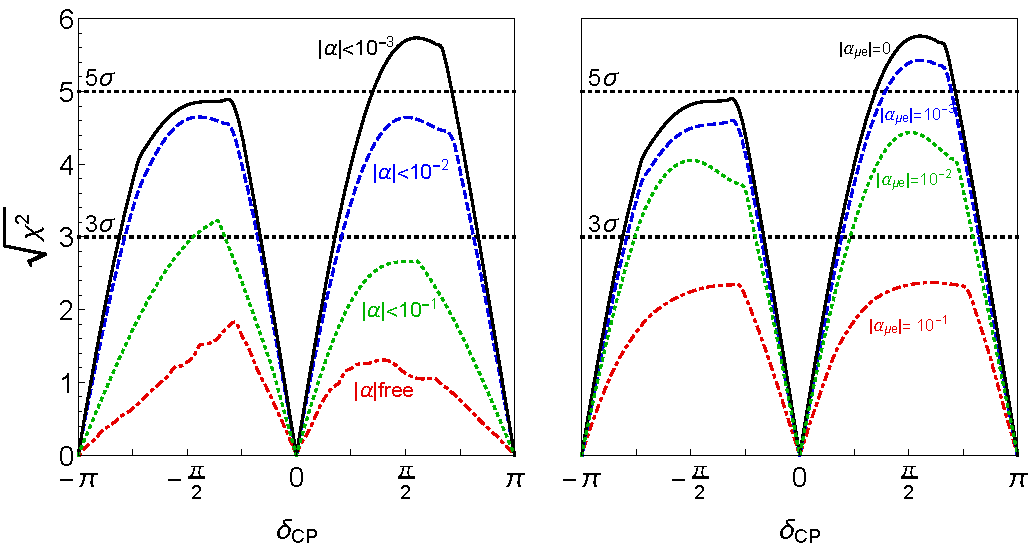
\includegraphics[width=0.8\columnwidth]{cpsens-comb.pdf}
\end{dunefigure}

\subsubsection{Conclusions}
A non-unitary lepton mixing matrix, as generally expected from the most common extensions of the \dword{sm}  explaining neutrino masses, would affect the neutrino oscillations to be measured by DUNE. The sensitivity that DUNE would provide to the non-unitarity parameters is comparable to that from present oscillation experiments, while not competitive to that from flavor and electroweak precision observables, which is roughly an order of magnitude more stringent. Conversely, the capability of DUNE to determine the standard oscillation parameters such as \dword{cpv} from $\delta_{CP}$ or the octant or maximality of $\theta_{23}$ would be seriously compromised by unitarity deviations in the \dword{pmns}. This negative impact is however significantly reduced when priors on the size of these deviations from other oscillation experiments are considered and disappears altogether if the more stringent constraints from flavor and electroweak precision data are added instead.

\begin{dunefigure}
[Expected frequentist allowed regions at the $1 \sigma$, $90\%$ and $2\sigma$ \dword{cl}]
{fig:octant}
{Expected frequentist allowed regions at the $1 \sigma$, $90\%$ and $2\sigma$ \dword{cl}\ for DUNE. All new physics parameters are assumed to be zero so as to obtain the expected non-unitarity sensitivities. The solid lines correspond to the analysis of DUNE data alone, while the dashed lines include the present constraints on non-unitarity.}
 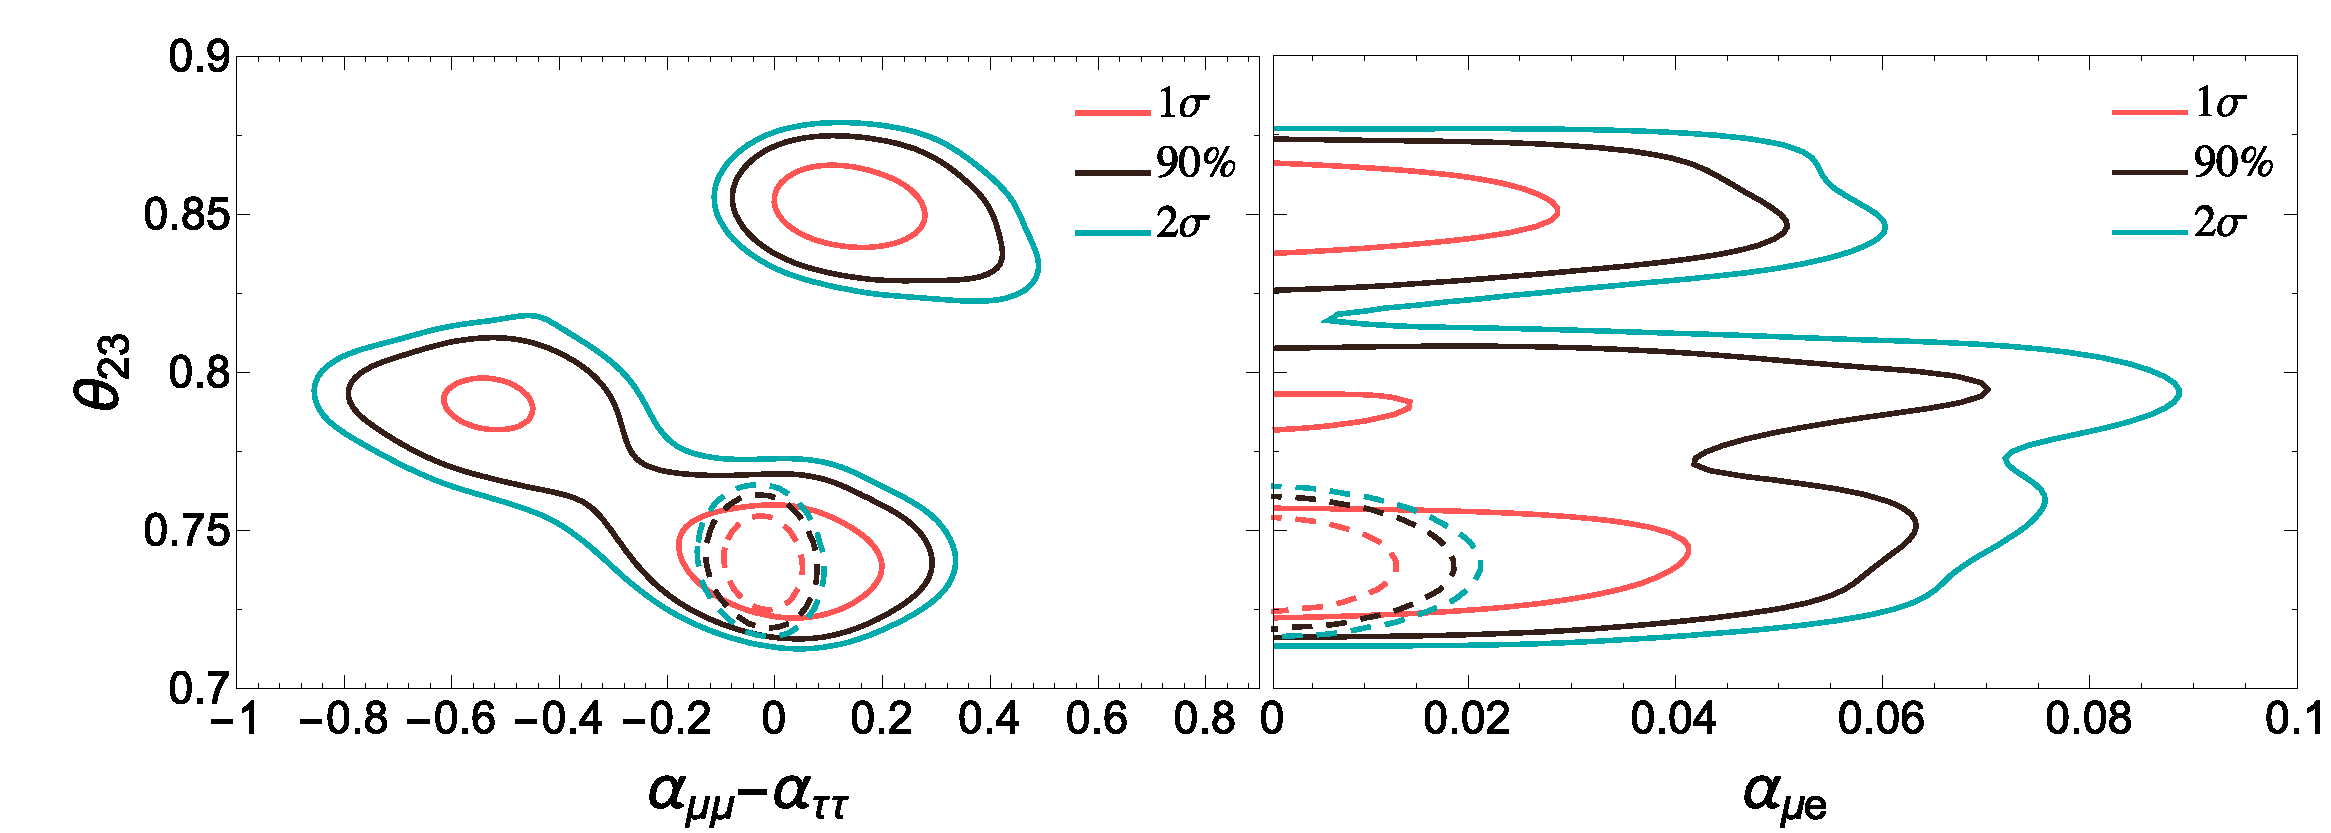
\includegraphics[width=0.8\columnwidth]{combined_pdf.pdf} 
\end{dunefigure}

\section{Non-Standard Neutrino Interactions}
\label{sec:nsi}
\dword{nsi} can significantly modify the data to be collected by DUNE as long as the new physics parameters are large enough. \dword{nsi} may impact the determination of current unknowns such as \dword{cpv}~\cite{Masud:2015xva,Masud:2016bvp}, mass hierarchy~\cite{Masud:2016gcl} and octant of $\theta_{23}$~\cite{Agarwalla:2016fkh}. If the DUNE data are consistent with the standard oscillation for three massive neutrinos, \dword{nc} \dword{nsi} effects of order 0.1 $G_F$, affecting neutrino propagation through the Earth, can be ruled out at DUNE~\cite{deGouvea:2015ndi,Coloma:2015kiu}. We notice that DUNE might improve current constraints on $|\epsilon^m_{e \tau}|$ and $|\epsilon^m_{e \mu}|$ by a factor 2-5~\cite{Ohlsson:2012kf,Miranda:2015dra,Farzan:2017xzy}. New  \dword{cc}  interactions can also lead to modifications in the production and the detection of neutrinos. The findings on source and detector \dword{nsi} studies at DUNE are presented in~\cite{Blennow:2016etl,Bakhti:2016gic}. In particular, the simultaneous impact on the measurement of $\delta_{\rm CP}$ and $\theta_{23}$ is investigated in detail. Depending on the assumptions, such as the use of the \dword{nd}  and whether \dword{nsi} at production and detection are the same, the impact of source/detector \dword{nsi} at DUNE may be relevant. We are assuming the results from~\cite{Blennow:2016etl}, in which DUNE does not have sensitivity to discover or to improve bounds on source/detector \dword{nsi}, and focus our attention in the propagation.

\subsection{NSI in propagation at DUNE}
%%%%%%%%%%%%%%%%%%%%%%%%%%%%%%%%%
%{\bf Authors: Chatterjee, Fernandez-Martinez, Forero, Guzzo, Kamiya, Miranda, Moura, Peres, Tortola, et al.}
\dword{nc} \dword{nsi} can be understood as non-standard
matter effects that are visible only in a \dword{fd} at a sufficiently long baseline. They can be parameterized as new contributions
to the \dword{msw} matrix in the neutrino-propagation Hamiltonian:
\begin{equation}
  H = U \left( \begin{array}{ccc}
           0 &                    & \\
             & \Delta m_{21}^2/2E & \\
             &                    & \Delta m_{31}^2/2E
         \end{array} \right) U^\dag + \tilde{V}_{\rm MSW} \,,
\end{equation}
with
\begin{equation}
  \tilde{V}_{\rm MSW} = \sqrt{2} G_F N_e
\left(
  \begin{array}{ccc}
    1 + \epsilon^m_{ee}       & \epsilon^m_{e\mu}       & \epsilon^m_{e\tau}  \\
        \epsilon^{m*}_{e\mu}  & \epsilon^m_{\mu\mu}     & \epsilon^m_{\mu\tau} \\
        \epsilon^{m*}_{e\tau} & \epsilon^{m*}_{\mu\tau} & \epsilon^m_{\tau\tau}
  \end{array} 
\right)
\label{eq:epsmatrix}
\end{equation}
Here, $U$ is the standard \dword{pmns} leptonic mixing matrix, for which we use the standard parameterization found, e.g., in~\cite{Agashe:2014yua}, 
and the $\epsilon$-parameters give the
magnitude of the \dword{nsi} relative to standard weak interactions.  For new physics scales of a few hundred GeV,  a value of $|\epsilon|$ of the order
%%%\lesssim 
0.01 or less is
expected~\cite{Davidson:2003ha,GonzalezGarcia:2007ib,Biggio:2009nt}. The DUNE
%%%\kmadj{1300} 
baseline provides an advantage in the detection of \dword{nsi} relative
to existing beam-based experiments with shorter baselines.
Only atmospheric-neutrino experiments have longer baselines, but the sensitivity of these experiments to \dword{nsi} is limited by systematic effects~\cite{Adams:2013qkq}.

To assess DUNE sensitivity to \dword{nc}  \dword{nsi}, the \dword{nsi} discovery reach is defined in the following way: the expected event spectra are simulated using  \dword{globes}~\cite{Huber:2004ka,Huber:2007ji}, assuming \textit{true} values for the  \dword{nsi} 
parameters, and a fit is then attempted assuming no \dword{nsi}. If the fit is
incompatible with the simulated data at a given confidence level,
the chosen \emph{true} values of the \dword{nsi} parameters are considered to be within the experimental discovery reach.

In this analysis, we use \dword{globes} with the Monte Carlo Utility Based Experiment Simulator (MonteCUBES) C library~\cite{Blennow:2009pk}, a plugin that replaces the deterministic  \dword{globes} minimizer by a Markov Chain Monte Carlo (MCMC) method that is able to handle higher dimensional parameter spaces. In the simulations we use the configuration for the DUNE \dword{cdr}~\cite{Alion:2016uaj}. Each point scanned by the MCMC is stored and a frequentist $\chi^2$ analysis is performed with the results. The analysis assumes an exposure of 300~kton.MW.year.

Considering that  \dword{nsi} exists, conducting the analysis with all the  \dword{nsi} parameters free to vary, we obtain the sensitivity regions in Figure~\ref{fig:nsi}. We omit the superscript $m$ that appears in eq.~\ref{eq:epsmatrix}. 
The credible regions are shown for different confidence level intervals.
\begin{dunefigure}
[Allowed regions for NSI parameters]
{fig:nsi}
{Allowed regions of the non-standard oscillation parameters in which we see important degeneracies (top) and the complex non-diagonal ones (bottom). We conduct the analysis considering all the \dword{nsi} parameters as non-negligible. The sensitivity regions are for 68\% CL [red line (left)], 90\% CL [green dashed line (middle)], and 95\% CL [blue dotted line (right)]. Current bounds are taken from~\cite{Gonzalez-Garcia:2013usa}.}
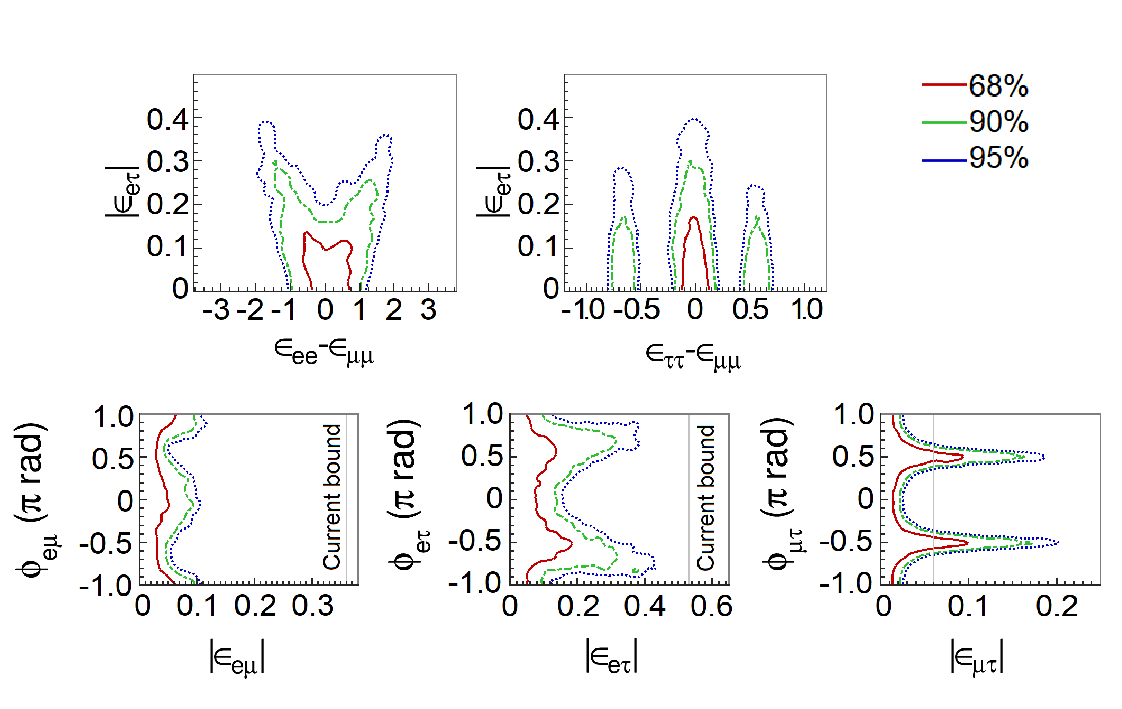
\includegraphics[width=0.8\columnwidth]{TDR12.pdf}
\end{dunefigure}
We note, however, that constraints on $\epsilon_{\tau\tau}-\epsilon_{\mu\mu}$ coming from global fit analysis~\cite{Gonzalez-Garcia:2013usa,Miranda:2015dra,Farzan:2017xzy,Esteban:2018ppq} can remove the left and right solutions of $\epsilon_{\tau\tau}-\epsilon_{\mu\mu}$ in Figure~\ref{fig:nsi}.

In order to constrain the standard oscillation parameters when  \dword{nsi} are %is 
present, we use the fit for three-neutrino mixing from~\cite{Gonzalez-Garcia:2013usa} and implement prior constraints to restrict the region sampled by the MCMC. The sampling of the parameter space is explained in~\cite{Coloma:2015kiu} and the priors that we use can be found in table~\ref{tab:priors1}.
\begin{dunetable}
[Oscillation parameters and priors implemented in MCMC.]
{| c | c | c |}
{tab:priors1}
{Oscillation parameters and priors implemented in MCMC for calculation of Figure~\ref{fig:nsi}.} 
{\bf Parameter} & {\bf Nominal} & {\bf 1$\sigma$ Range ($\pm$) }\\ \toprowrule
$\theta_{12}$ &0.19$\pi~\textrm{rad}$&2.29\%\\ \colhline
$\sin^2(2\theta_{13})$ &0.08470&0.00292\\ \colhline
$\sin^2(2\theta_{23})$ &0.9860&0.0123\\ \colhline
$\Delta m^2_{21} $ &7.5 $\times10^{-5}\textrm{eV}^2$&2.53\%\\ \colhline
$\Delta m^2_{31} $ &2.524 $\times10^{-3}\textrm{eV}^2$&free\\ \colhline
$\delta_{\rm CP} $ &1.45$\pi~\textrm{rad}$&free\\
\end{dunetable}

Then we can observe the effects of \dword{nsi} on the measurements of the standard oscillation parameters at DUNE. In Figure~\ref{fig:standar-nsi}, we superpose the allowed regions with non-negligible  \dword{nsi} and the standard-only credible regions at 90\% \dword{cl}. %There is an important degeneracy that 
An important degeneracy appears in the measurement of the mixing angle $\theta_{23}$. We also see that the sensitivity of the \dword{cp} phase is strongly affected.
\begin{dunefigure}
[Projections of the standard oscillation parameters with nonzero NSI]
{fig:standar-nsi}
{Projections of the standard oscillation parameters with nonzero \dword{nsi}. The sensitivity regions are for 68\%, 90\%, and 95\% \dword{cl}. The allowed regions considering negligible \dword{nsi} (standard oscillation (SO)) are superposed to the SO+NSI at 90\% \dword{cl}.}
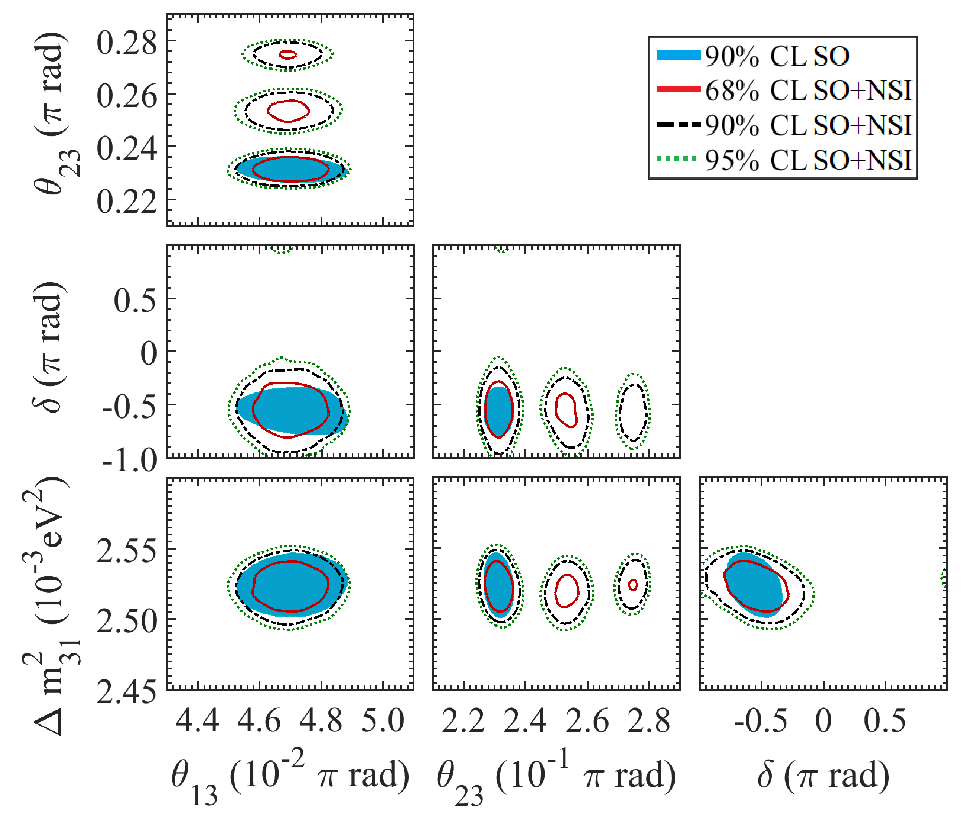
\includegraphics[width=0.6\columnwidth]{TDR10.pdf}
\end{dunefigure}

%%%%%%%%%%%%%%%%%%%%%%%%%%%%%%%%%%%%%%%%%%%%%%%%%%%%%%%%%%%%%%
\subsection{Effects of baseline and matter-density variation on  NSI measurements}\label{ssec:matter}
%%%%%%%%%%%%%%%%%%%%%%%%%%%%%%%%%%%%%%%%%%%%%%%%%%%%%%%%%%%%%%
The effects of matter density variation and its average along the beam path from \fnal to \surf  were studied considering the standard neutrino oscillation framework with three flavors~\cite{Roe:2017zdw,Kelly:2018kmb}. In order to obtain the results of Figures~\ref{fig:nsi} and~\ref{fig:standar-nsi}, we use a high-precision calculation for the baseline of \SI{1284.9}{km} and the average density of \SI{2.8482}{g/cm^3}~\cite{Roe:2017zdw}.

The DUNE collaboration has been using the so-called PREM~\cite{Dziewonski:1981xy,PREM2} density profile to consider matter density variation. With this assumption, the neutrino beam crosses a few constant density layers.
However, a more detailed density map is available for the USA with more than 50 layers and $0.25 \times 0.25$ degree cells of latitude and longitude: The Shen-Ritzwoller or S.R. profile~\cite{SR:2016,Roe:2017zdw}. Comparing the S.R. with the PREM profiles, Kelly and Parke~\cite{Kelly:2018kmb} show that, in the standard oscillation paradigm, DUNE is not highly sensitive to the density profile and that the only oscillation parameter with its measurement slightly impacted by the average density true value is \deltacp{}.
\dword{nsi}, however, may be sensitive to the profile, particularly considering the phase $\phi_{e\tau}$~\cite{Chatterjee:2018dyd}, to which DUNE will have a high sensitivity~\cite{Ohlsson:2012kf,Miranda:2015dra,deGouvea:2015ndi,Coloma:2015kiu,Farzan:2017xzy}, as we also see in Figure~\ref{fig:nsi}.

In order to compare the results of our analysis predictions for DUNE with the constraints from other experiments we use the results from~\cite{Farzan:2017xzy}. There are differences in the parameter nominal values used for calculating the $\chi^2$ function and other assumptions. This is the reason why the regions in Figure~\ref{fig:bars} do not have the same central values, but this comparison gives a good view of how DUNE can substantially improve the bounds on, for example, $\varepsilon_{\tau\tau}-\varepsilon_{\mu\mu}$, $\Delta m^2_{31}$, and the non-diagonal \dword{nsi} parameters.

\begin{dunefigure}
[1D DUNE constraints versus current constraints]
{fig:bars}
{One-dimensional DUNE constraints compared with current constraints calculated in \cite{Farzan:2017xzy}. See text for details.}
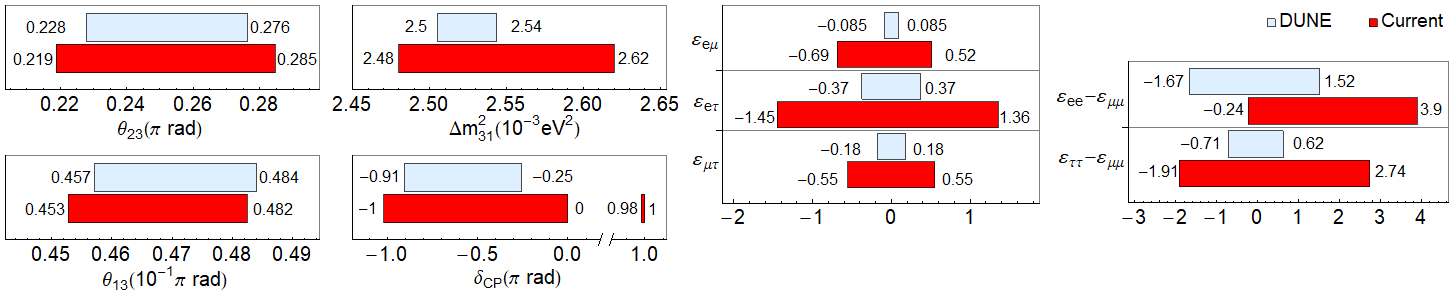
\includegraphics[width=1.0\columnwidth]{graphics/Barras_Geral_dune.png}
\end{dunefigure}


\subsubsection{Conclusions and prospects}
\dword{nsi} can significantly impact the determination of current unknowns such as \dword{cpv} and the octant of $\theta_{23}$. Clean determination of the intrinsic \dword{cp} phase at long-baseline experiments such as DUNE is a formidable task~\cite{Rout:2017udo}. A feasible strategy to extricate physics scenarios at DUNE using high-energy beams was suggested in~\cite{Masud:2017bcf}.


%%%%%%%%%%%%%%%%%%%%%%%%%
\section{CPT Symmetry Violation}
%{\bf Authors: Barenboim, Ternes, and Tórtola.}

\dword{cpt} symmetry, the combination of charge conjugation, parity and time reversal, is a cornerstone of our model-building strategy. 
DUNE can improve the present limits on Lorentz and \dword{cpt} violation by several orders of magnitude~\cite{Streater:1989vi,Barenboim:2002tz,Kostelecky:2003cr,Diaz:2009qk,Kostelecky:2011gq,Barenboim:2017ewj}, contributing as a very important experiment to test these fundamental assumptions underlying quantum field theory.

%
\dword{cpt} invariance is one of the predictions of major importance of local, relativistic quantum field theory. One of the predictions of \dword{cpt} invariance is that particles and antiparticles have the same masses and, if unstable, the same lifetimes. To prove the \dword{cpt} theorem one needs only three ingredients~\cite{Streater:1989vi}: Lorentz invariance, hermiticity of the Hamiltonian, and locality.
%

Experimental bounds on \dword{cpt} invariance can be derived using the neutral kaon system~\cite{Schwingenheuer:1995uf}:
%
\begin{equation}
  \frac{|m(K^0) - m(\overline{K}^0)|}{m_K} < 0.6 \times 10^{-18}\,. 
  \label{eq:mK}
\end{equation}
%
This result, however, should be interpreted very carefully for two reasons. First, we do not have a complete theory of \dword{cpt} violation, and it is therefore arbitrary to take the kaon-mass as a scale. Second, since kaons are bosons, the term entering the Lagrangian is the mass squared and not the mass itself. With this in mind, we can rewrite the previous bound as:
%
%\begin{equation}
 $ |m^2(K^0) - m^2(\overline{K}^0)| < 0.3~\mbox{eV}^2 \, $.
%  \label{eq:mK2}
%\end{equation}
%
Here we %will 
see that neutrinos can test the predictions of the \dword{cpt} theorem to an unprecedented extent and could, therefore, provide stronger limits than the ones regarded as the most stringent ones %by now
to date\footnote{\dword{cpt} was tested also using charged leptons. However, these measurements involve a combination
of mass and charge and are not a direct \dword{cpt} test. Only neutrinos can provide \dword{cpt} tests on an elementary mass not contaminated by charge.}. 
%
In the absence of a solid model of flavor, not to mention one of \dword{cpt} violation, the spectrum  of neutrinos and antineutrinos can differ both  in the mass eigenstates themselves as well as in the flavor composition of each of these states. It is important to notice then that neutrino oscillation experiments can only test \dword{cpt} in the mass differences and mixing angles. An overall shift between the neutrino and antineutrino spectra will be missed by oscillation experiments.  Nevertheless, such a pattern can be bounded by cosmological data~\cite{Barenboim:2017vlc}. Unfortunately direct searches for neutrino mass (past, present, and future) involve only antineutrinos and hence cannot be used to draw any conclusion on \dword{cpt} invariance on the absolute mass scale, either.
%
Therefore, using neutrino oscillation data, we will compare the mass splittings and mixing angles of  neutrinos with those of antineutrinos. Differences in the neutrino and antineutrino spectrum would imply the violation of the \dword{cpt} theorem.

In Ref.~\cite{Barenboim:2017ewj} the authors derived the most up-to-date bounds on \dword{cpt} invariance from the neutrino sector %. The data used to derive these bounds are the same considered in the global fit to neutrino oscillations in Ref.~\cite{deSalas:2017kay}. 
using the same data that was used in the global fit to neutrino oscillations in Ref.~\cite{deSalas:2017kay}. 
Of course, experiments that cannot distinguish between neutrinos and antineutrinos, such as atmospheric data from \superk~\cite{Abe:2017aap}, IceCube-DeepCore~\cite{Aartsen:2014yll,Aartsen:2017nmd} and ANTARES~\cite{AdrianMartinez:2012ph} were not included. The complete data set used, as well as the parameters to which they are sensitive, are % the following:
%
%\begin{itemize}
 (1) from solar neutrino data~\cite{Cleveland:1998nv,Kaether:2010ag,Abdurashitov:2009tn,hosaka:2005um,Cravens:2008aa,Abe:2010hy,Nakano:PhD,Aharmim:2008kc,Aharmim:2009gd,Bellini:2013lnn}:  $\theta_{12}$, $\Delta m_{21}^2$, and $\theta_{13}$;
 (2) from neutrino mode in long-baseline experiments K2K~\cite{Ahn:2006zza}, MINOS~\cite{Adamson:2013whj,Adamson:2014vgd}, T2K~\cite{Abe:2017uxa,Abe:2017bay}, and NO$\nu$A~\cite{Adamson:2017qqn,Adamson:2017gxd}:  $\theta_{23}$, $\Delta m_{31}^2$, and $\theta_{13}$;
 (3) from KamLAND reactor antineutrino data~\cite{Gando:2010aa}: $\overline{\theta}_{12}$, $\Delta \overline{m}_{21}^2$, and $\overline{\theta}_{13}$;
 (4) from short-baseline reactor antineutrino experiments Daya Bay~\cite{An:2016ses}, RENO~\cite{RENO:2015ksa}, and Double Chooz~\cite{Abe:2014bwa}:     $\overline{\theta}_{13}$ and $\Delta \overline{m}_{31}^2$; and 
 (5) from antineutrino mode in long-baseline experiments MINOS~\cite{Adamson:2013whj,Adamson:2014vgd} and T2K~\cite{Abe:2017uxa,Abe:2017bay}: $\overline{\theta}_{23}$, $\Delta \overline{m}_{31}^2$, and
$\overline{\theta}_{13}$\footnote{The K2K experiment took  data only in neutrino mode, while the \nova experiment had not published data in the antineutrino mode when these bounds were calculated.}. %\\
%\end{itemize}

From the analysis of all previous data samples, one can derive the most up-to-date bounds on \dword{cpt} violation:
%
% \begin{eqnarray}
$ |\Delta m_{21}^2-\Delta \overline{m}_{21}^2| < 4.7\times 10^{-5} \,  \text{eV}^2,\,\,
%  \nonumber \\
 |\Delta m_{31}^2-\Delta \overline{m}_{31}^2| < 3.7\times 10^{-4} \, \text{eV}^2,\,\,
% \nonumber \\
 |\sin^2\theta_{12}-\sin^2\overline{\theta}_{12}| < 0.14\,,\,\,
%  \\
 |\sin^2\theta_{13}-\sin^2\overline{\theta}_{13}| < 0.03\,, \,\,
%  \nonumber \\
 {\rm and}~|\sin^2\theta_{23}-\sin^2\overline{\theta}_{23}| < 0.32\,.
 $  %\\
 %\nonumber.
% \label{eq:new-bounds}
% \end{eqnarray} 

At the moment it is not possible to set any bound on $|\delta-\overline{\delta}|$, since all possible values of
$\delta$ or $\overline{\delta}$ are allowed by data. The preferred intervals of $\delta$ obtained in Ref.~\cite{deSalas:2017kay} can only be obtained after combining the neutrino and antineutrino data samples. 
The limits  on $\Delta(\Delta m_{31}^2)$ and $\Delta(\Delta m_{21}^2)$  are already better than the one derived from the neutral kaon system and should be regarded as the best current bounds on \dword{cpt} violation on the mass squared. % so far. 
Note that these results were derived assuming the same mass ordering for neutrinos and antineutrinos. If the ordering was different for neutrinos and antineutrinos, this would be an indication for \dword{cpt} violation on its own. In the following we show how DUNE could improve this bound.

\subsubsection{Sensitivity to \dword{cpt} symmetry violation in the neutrino sector}
\label{sec:sensitivity}

\begin{dunetable}
[Oscillation parameters used to simulate (anti)neutrino data.]
{| c | c |}
{tab:par2}
{Oscillation parameters used to simulate neutrino and antineutrino data analyzed in Section~\ref{sec:sensitivity}.}
    {\bf Parameter} & {\bf Value}  \\ \toprowrule
    $\Delta m^2_{21}$& $7.56\times 10^{-5}\text{eV}^2$\\  \colhline
    %%
    $\Delta m^2_{31}$&  $2.55\times 10^{-3}\text{eV}^2$\\  \colhline
    %%	
    $\sin^2\theta_{12}$ & 0.321\\  \colhline
    $\sin^2\theta_{23}$ &  0.43, 0.50, 0.60\\  \colhline
    $\sin^2\theta_{13}$ & 0.02155\\  \colhline
    $\delta$ & 1.50$\pi$\\
\end{dunetable}

Here we study the sensitivity of the DUNE experiment to measure \dword{cpt} violation in the neutrino sector by analyzing neutrino and antineutrino oscillation parameters separately. We assume the neutrino oscillations being parameterized by the usual \dword{pmns} matrix $U_{\text{PMNS}}$, with parameters $\theta_{12},\theta_{13},\theta_{23},\Delta m_{21}^2,\Delta m_{31}^2, {\rm and}~\delta$, while the antineutrino oscillations are parameterized by a matrix $\overline{U}_{\text{PMNS}}$ with parameters $\overline{\theta}_{12},\overline{\theta}_{13},\overline{\theta}_{23},\Delta \overline{m}_{21}^2,\Delta \overline{m}_{31}^2, {\rm and}~\overline{\delta}$. Hence, antineutrino oscillation is described  by the same probability functions as neutrinos with the neutrino parameters replaced by their antineutrino counterparts\footnote{Note that the antineutrino oscillation probabilities also include the standard change of sign in the \dword{cp} phase.}. 
To simulate the future neutrino data signal in DUNE, we assume the true values for neutrinos and antineutrinos to be as listed in Table~\ref{tab:par2}.
Then, in the statistical analysis, we vary freely all the oscillation parameters, except the solar ones, which are fixed to their best fit values throughout the simulations. Given the great precision in the determination of the reactor mixing angle by the short-baseline reactor experiments~\cite{An:2016ses,RENO:2015ksa,Abe:2014bwa}, in our analysis we use a prior on $\overline{\theta}_{13}$, but not on $\theta_{13}$. We also consider three different values for the atmospheric angles, as indicated in Table~\ref{tab:par2}. The exposure considered in the analysis corresponds to 300~kton.MW.year.

Therefore, to test the sensitivity at DUNE we perform the simulations assuming $\Delta x = |x-\overline{x}| = 0$, where $x$ is any of the oscillation parameters. Then we estimate the sensitivity to $\Delta x\neq 0$. To do so we calculate two $\chi^2$-grids, one for neutrinos and one for antineutrinos, varying the four parameters of interest. After minimizing over all parameters except $x$ and $\overline{x}$, we calculate 
%
\begin{equation}
 \chi^2(\Delta x) = \chi^2(|x-\overline{x}|) = \chi^2(x)+\chi^2(\overline{x}),
 \label{eq:chi2-nu-nubar}
\end{equation}
%
where we have considered all the possible combinations of $|x-\overline{x}|$. The results are presented in Figure~\ref{fig:sensitivity-CPT}, where we plot three different lines, labelled as ``high'', ``max'' and ``low.'' These refer to the assumed value for the atmospheric angle: in the lower octant (low), maximal mixing (max) or in the upper octant (high). Here we can see that there is sensitivity neither to $\Delta(\sin^2\theta_{13})$, where the 3$\sigma$ bound would be of the same order %of 
as the current measured value for $\sin^2\overline{\theta}_{13}$, nor to $\Delta\delta$, where no single value of the parameter would be excluded at more than 2$\sigma$.

On the contrary, interesting results for $\Delta(\Delta m_{31}^2)$ and $\Delta(\sin^2\theta_{23})$ are obtained. First, we see that DUNE can put stronger bounds on the difference of the atmospheric mass splittings, namely $\Delta(\Delta m_{31}^2) < 8.1\times 10^{-5}$, improving the current neutrino bound by one order of magnitude. For the atmospheric angle, we obtain different results depending on the true value assumed in the simulation of DUNE data. In the lower right panel of Figure~\ref{fig:sensitivity-CPT} we see the different behavior obtained for $\theta_{23}$ with the values of $\sin^2\theta_{23}$ from table~\ref{tab:par2}, i.e., lying in the lower octant, being maximal, and lying in the upper octant.
%\fixme{clarify previous sentence. (anne) -->> Depending on the TRUE value of the atmospheric angle the discrimination power changes.}
As one might expect, the sensitivity increases with $\Delta\sin^2\theta_{23}$ in the case of maximal mixing. However, if the true value lies in the lower or upper octant, a degenerate solution appears in the complementary octant.
\begin{figure}[!htb]
 \centering
        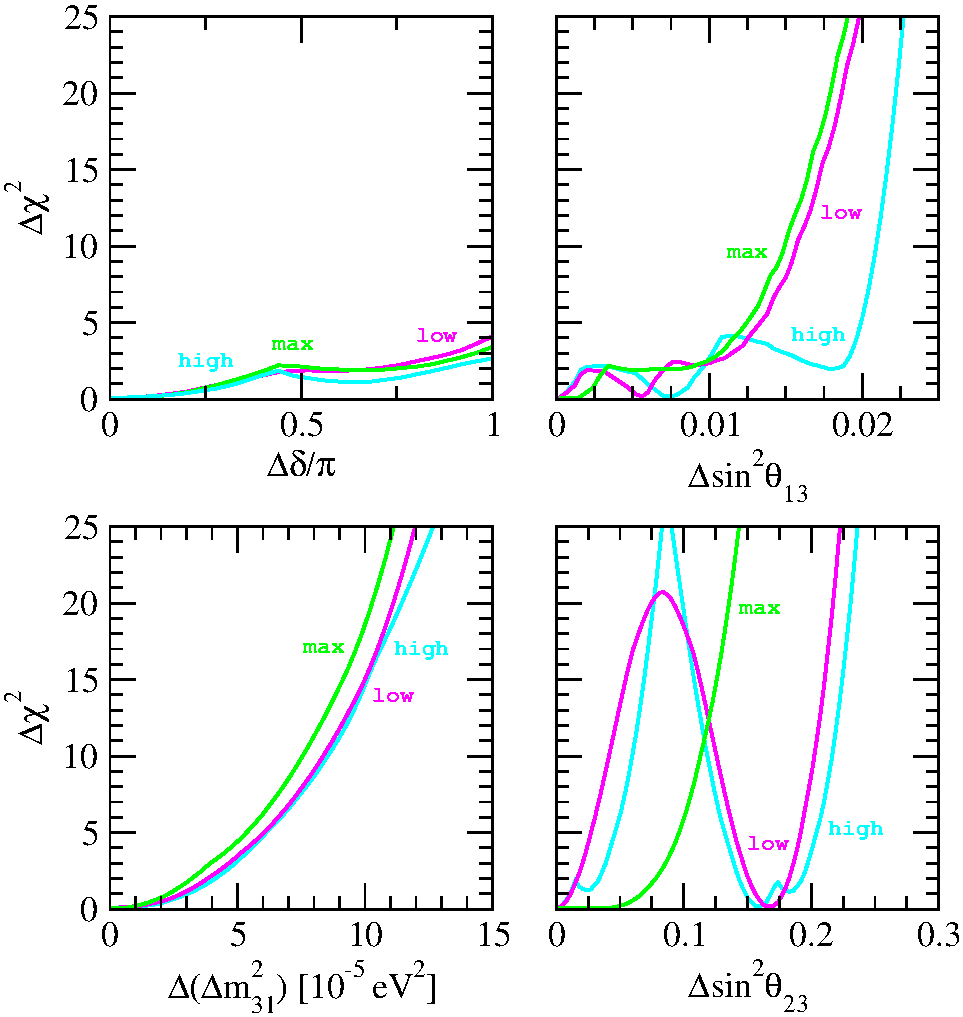
\includegraphics[width=0.55\columnwidth]{sensitivity-CPT.pdf}
        \caption[Sensitivities to the difference of neutrino and antineutrino parameters]{The sensitivities of DUNE to the difference of neutrino and antineutrino parameters: 
        $\Delta\delta$, $\Delta(\Delta m_{31}^2)$, $\Delta(\sin^2\theta_{13})$ and $\Delta(\sin^2\theta_{23})$  
        for the atmospheric angle in the lower octant (magenta line),  in the upper octant (cyan line) and for maximal mixing (green line).}
	\label{fig:sensitivity-CPT}
\end{figure}

\subsection{Imposter solutions}
\label{sec:impost}
In %different 
some types of neutrino oscillation experiments, e.g., accelerator experiments, neutrino and antineutrino data are obtained in separate experimental runs. The usual procedure followed by the experimental collaborations, as well as the global oscillation fits as for example Ref.~\cite{deSalas:2017kay}, assumes \dword{cpt} invariance and analyzes the full data sample in a joint way.
%\fixme{I'm trying to parse this. Is this right? ``Experimental collaborations usually assume \dword{cpt} invariance and analyze the full data sample in a holistic way. Global oscillation fits, e.g., by~\cite{deSalas:2017kay}, are usually done following a similar procedure.''
%-->> Absolutely. This is how fits are done: CPT assumed}
However, if \dword{cpt} is violated in nature, the outcome of the joint data analysis might give rise to what we call an ``imposter'' solution, i.e., one that does not correspond to the true solution of any channel. 

Under the assumption of \dword{cpt} conservation, the $\chi^2$ functions are computed according to
%
\begin{equation}
 \chi^2_{\text{total}}=\chi^2(\nu)+\chi^2(\overline{\nu})\, ,
 \label{eq:CPT-cons}
\end{equation}
%
and assuming that the same parameters describe neutrino and antineutrino flavor oscillations. In contrast, in Eq.~(\ref{eq:chi2-nu-nubar}) we first profiled over the parameters in neutrino and antineutrino mode separately and then added the profiles. Here, we shall assume \dword{cpt} to be violated in nature, but perform our analysis as if it were conserved. As an example, we assume that the true value for the atmospheric neutrino mixing is $\sin^2\theta_{23}=0.5$, while the antineutrino mixing angle is given by $\sin^2\overline{\theta}_{23}=0.43$. The rest of the oscillation parameters are set to the values in Table~\ref{tab:par2}. Performing the statistical analysis in the \dword{cpt}-conserving way, as indicated in Eq.~(\ref{eq:CPT-cons}), we obtain the profile of the atmospheric mixing angle presented in Figure~\ref{fig:imposter-sq23}. The profiles for the individual reconstructed results (neutrino and antineutrino) are also shown in the figure for comparison.
%As can be seen, we obtain
The result is a new best fit value at $\sin^2\theta^\text{comb}_{23}=0.467$, disfavoring the true values for neutrino and antineutrino parameters at approximately 3$\sigma$ and more than 5$\sigma$, respectively. 

\begin{figure}[!htb]
 \centering
        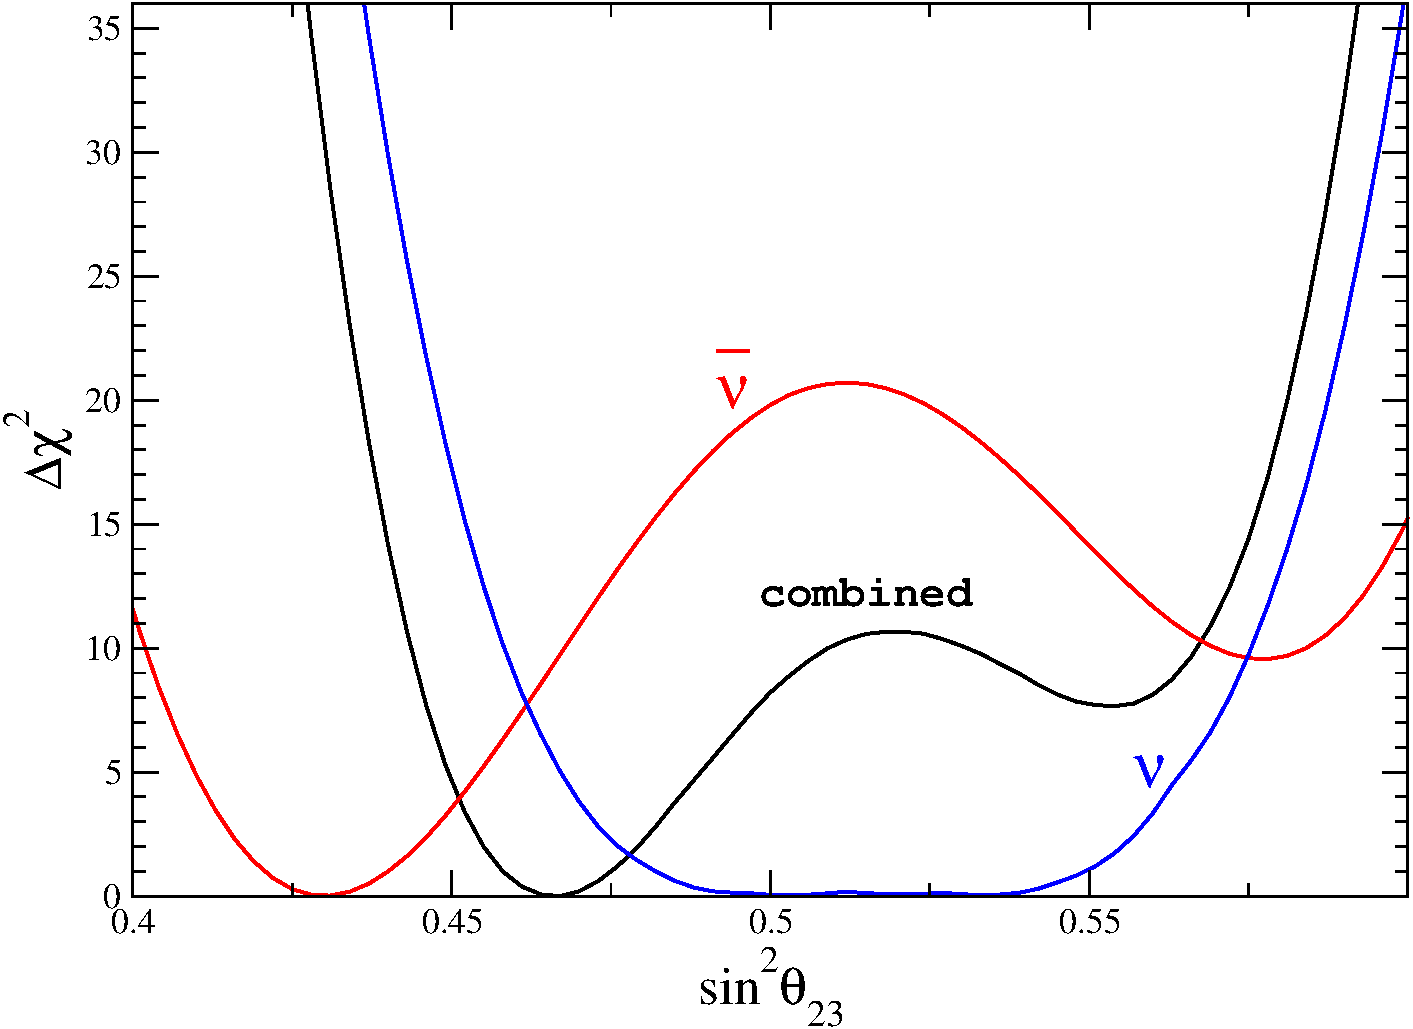
\includegraphics[width=0.45\columnwidth]{imposter-sq23.pdf}
        \caption[Sensitivity to $\theta_{23}$ for (anti)neutrinos, and combination under CPT conservation]{DUNE sensitivity to the atmospheric angle for neutrinos (blue), antineutrinos (red), and to the combination of both under the assumption of \dword{cpt} conservation (black).
         }
	\label{fig:imposter-sq23}
\end{figure}

%%%%%%%%%%%%%%%%%%%%%%%%%%%%%%%%%%%%%%%%%%%%%%%%%%
%%% NEUTRINO TRIDENTS %%%%%%%%%%%%%%%%%%%%%%%%%%%%
\section{Search for Neutrino Tridents at the Near Detector}
%%%
Neutrino trident production is a weak process in which a neutrino, scattering off the Coulomb field of a heavy nucleus, generates a pair of charged leptons, as shown in Fig.~\ref{fig:diagrams}~\cite{Czyz:1964zz,Lovseth:1971vv,Fujikawa:1971nx,Koike:1971tu,Koike:1971vg,Brown:1973ih,Belusevic:1987cw}.
\begin{figure}[!hb]
\centering
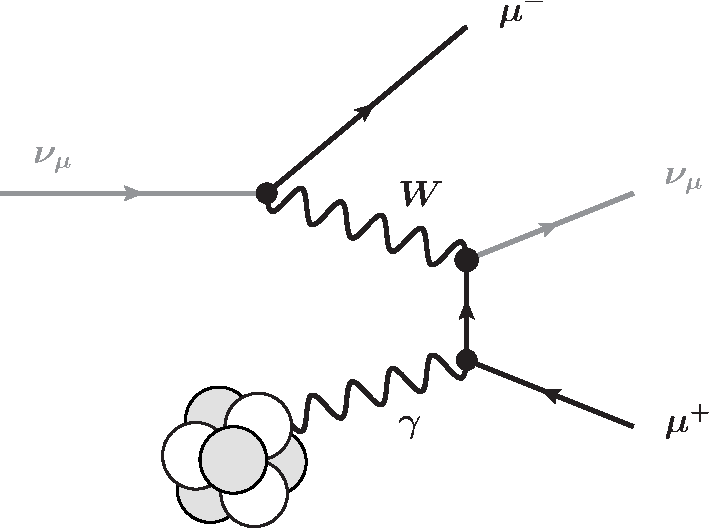
\includegraphics[width=0.27\textwidth]{trident_diagram_mumu_W.pdf} \qquad
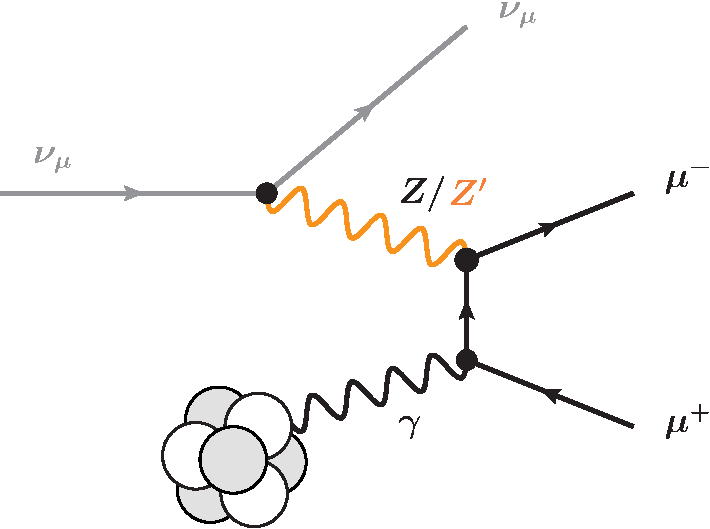
\includegraphics[width=0.27\textwidth]{trident_diagram_mumu_Zprime.pdf} \\[\baselineskip]
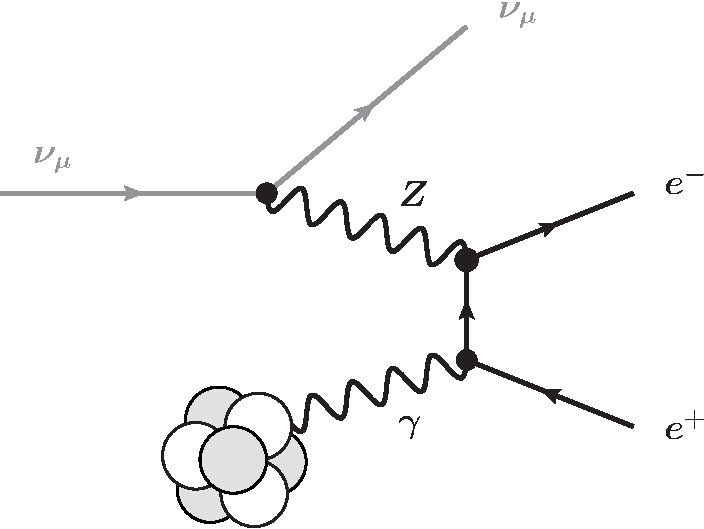
\includegraphics[width=0.27\textwidth]{trident_diagram_ee_Z.pdf} \qquad
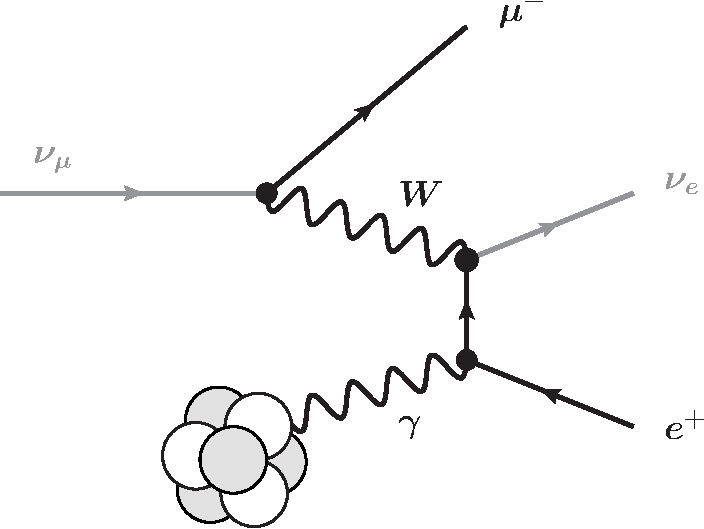
\includegraphics[width=0.27\textwidth]{trident_diagram_mue_W.pdf} \\[\baselineskip]
\caption[Example diagrams for $\numu$-induced trident processes in the SM]{Example diagrams for muon-neutrino-induced trident processes in the Standard Model. A second set of diagrams where the photon couples to the negatively charged leptons is not shown. 
Analogous diagrams exist for processes induced by different neutrino flavors and by anti-neutrinos. A diagram illustrating trident interactions mediated by a new $Z'$ gauge boson, discussed in the text, is shown on the top right.}
\label{fig:diagrams}
\end{figure}
Measurements of muonic neutrino tridents ($\nu_\mu \to \nu_\mu \mu^+\mu^-$) were carried out at the CHARM-II~\cite{Geiregat:1990gz}, CCFR~\cite{Mishra:1991bv} and NuTeV~\cite{Adams:1999mn} experiments:
\[
\frac{\sigma(\nu_\mu \to \nu_\mu \mu^+\mu^-)_\text{exp}}{\sigma(\nu_\mu \to \nu_\mu \mu^+\mu^-)_\text{SM}} = 
\begin{cases}
1.58 \pm 0.64         & \text{(CHARM-II)} \\ 
0.82 \pm 0.28         & \text{(CCFR)} \\
0.72 ^{+1.73}_{-0.72} & \text{(NuTeV)} 
\end{cases}
\]
The high-intensity muon-neutrino beam at the DUNE \dword{nd}  will lead to a sizable production rate of trident events (see Table~\ref{tab:trident_rates}), offering excellent prospects to improve the above measurements~\cite{Altmannshofer:2019zhy,Ballett:2018uuc,Ballett:2019xoj}. A deviation from the event rate predicted by the \dword{sm} could be an indication of new interactions mediated by the corresponding new gauge bosons~\cite{Altmannshofer:2014pba}. 

%%%%%%%%%%%%%%%%%%%%%%%%%%%%%%
\begin{dunetable}
[Expected number of SM $\nu_\mu$ and $\bar\nu_\mu$-induced trident events at ND per ton of Ar per year]
{|l|c|c|}
{tab:trident_rates}
{Expected number of \dword{sm} $\nu_\mu$ and $\bar\nu_\mu$-induced trident events at the LArTPC of the DUNE \dword{nd} per metric ton of argon and year of operation.}
{\bf Process} & {\bf Coherent} & {\bf Incoherent} \\ \toprowrule
\midrule
$\nu_\mu \to \nu_\mu \mu^+\mu^-$ & $1.17 \pm 0.07$ & $0.49 \pm 0.15$ \\
$\nu_\mu \to \nu_\mu e^+e^-$ & $2.84 \pm 0.17$ & $0.18 \pm 0.06$\\
$\nu_\mu \to \nu_e e^+\mu^-$ & $9.8 \pm 0.6$ & $1.2 \pm 0.4$ \\
$\nu_\mu \to \nu_e \mu^+e^-$ & $0$ & $0$ \\
\midrule
$\bar\nu_\mu \to \bar\nu_\mu \mu^+\mu^-$ & $0.72 \pm 0.04$ & $0.32 \pm 0.10$ \\
$\bar\nu_\mu \to \bar\nu_\mu e^+e^-$ & $2.21 \pm 0.13$ & $0.13 \pm 0.04$ \\
$\bar\nu_\mu \to \bar\nu_e e^+\mu^-$ & $0$ & $0$ \\
$\bar\nu_\mu \to \bar\nu_e \mu^+e^-$ & $7.0 \pm 0.4$ & $0.9 \pm 0.3$ \\
\end{dunetable}
%%%%%%%%%%%%%%%%%%%%%%%%%%%%%%


The main challenge in obtaining a precise measurement of the muonic trident cross section will be the copious backgrounds, mainly consisting of \dword{cc} single-pion production events, $\nu_\mu N \to \mu \pi N^\prime$, as muon and pion tracks can be easily confused in LArTPC detectors. The discrimination power of the DUNE \dword{nd} LArTPC was evaluated using large simulation datasets of signal and background. Each simulation event represents a different neutrino-argon interaction in the active volume of the detector. Signal events were generated using a standalone code \cite{Altmannshofer:2019zhy} that simulates trident production of muons and electrons through the scattering of $\nu_{\mu}$ and $\nu_e$ on argon nuclei (or iron nuclei, for comparison with CCFR and NuTeV results). The generator considers both the coherent scattering on the full nucleus (the dominant contribution) and the incoherent scattering on individual nucleons. Background events, consisting of several \dword{sm} neutrino interactions, were generated using \dword{genie}. Roughly $38\%$ of the generated events have a charged pion in the final state, leading to two charged tracks with muon-like energy deposition pattern ($\mathrm{d}E/\mathrm{d}x$), as in our trident signal. All final-state particles produced in the interactions were propagated through the detector geometry using the Geant4-based \cite{Agostinelli:2002hh,Allison:2006ve,Allison:2016lfl} simulation of the DUNE \dword{nd}. Charge collection and readout were not simulated, and possible inefficiencies due to misreconstruction effects or event pile-up were disregarded for simplicity.

%%%%%%%%%%%%%%%%%%%%%%%%%%%%%%
\begin{figure}[!tb]
\centering
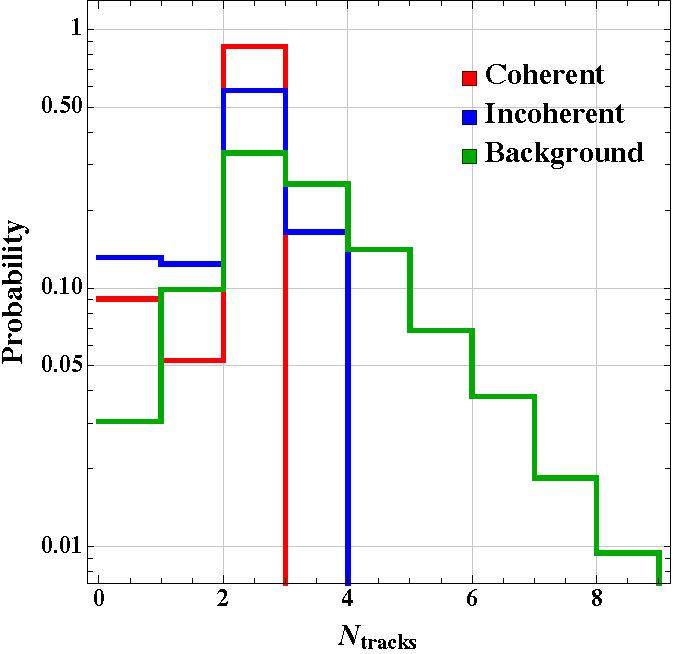
\includegraphics[height=5cm]{NTracksHistogram.pdf}
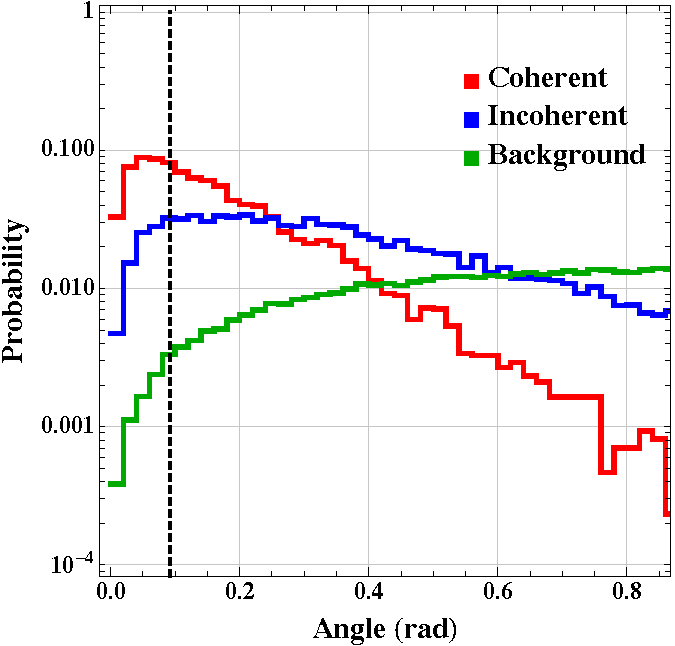
\includegraphics[height=5cm]{AngleHistogram.pdf} \\[0.75\baselineskip]
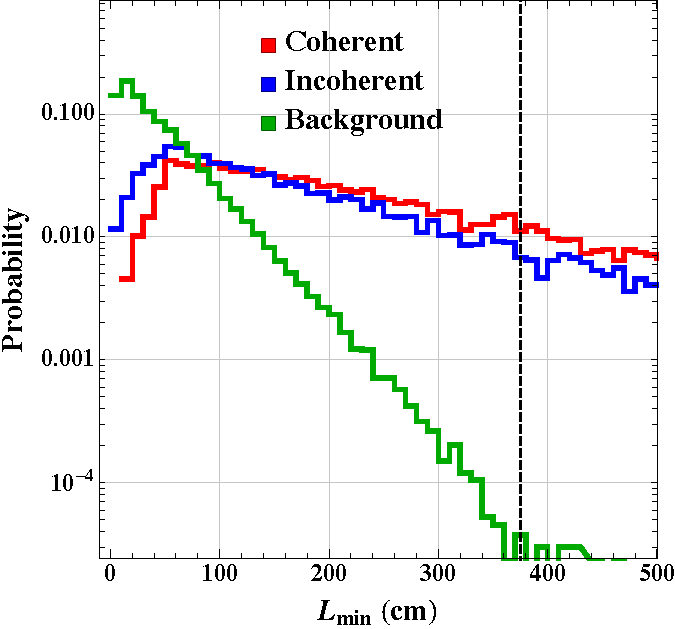
\includegraphics[height=5cm]{LengthHistogram.pdf}
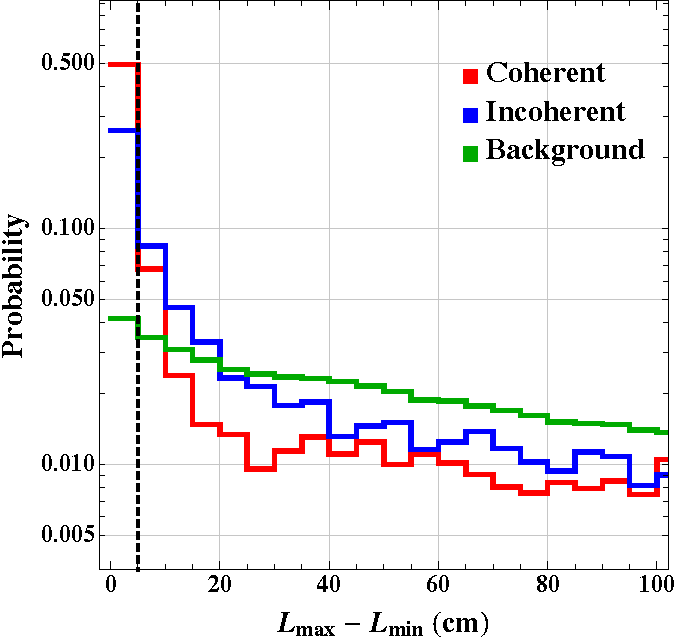
\includegraphics[height=5cm]{DeltaLHistogram.pdf}
\caption[%Kinematic distributions of s
Signal and background %considered 
for selecting %the selection of 
muonic trident interactions in ND LArTPC]{Event kinematic distributions of signal and background considered for the selection of muonic trident interactions in the \dword{nd} \dword{lartpc}: number of tracks (top left), angle between the two main tracks (top right), length of the shortest track (bottom left), and the difference in length between the two main tracks (bottom right). The dashed, black vertical lines indicate the optimal cut values used in the analysis.} \label{fig:trident_kinematics}
\end{figure}
%%%%%%%%%%%%%%%%%%%%%%%%%%%%%%

Figure~\ref{fig:trident_kinematics} shows the distribution (area normalized) for signal and background of the different kinematic variables used in our analysis for the discrimination between signal and background. As expected, background events tend to contain a higher number of tracks than the signal. The other distributions also show a clear discriminating power: the angle between the two tracks is typically much smaller in the signal than in the background. Moreover, the signal tracks (two muons) tend to be longer than tracks in the background (mainly one muon plus one pion).

%%%%%%%%%%%%%%%%%%%%%%%%%%%%%%%%%%%%%%%%
\subsection{Sensitivity to new physics} 
The sensitivity of neutrino tridents to heavy new physics (i.e., heavy compared to the momentum transfer in the process) can be parametrized in a model-independent way using a modification of the effective four-fermion interaction Hamiltonian. Focusing on the case of muon-neutrinos interacting with muons, the vector and axial-vector couplings can be written as
%%%%%%%%%%
\begin{equation}
g_{\mu\mu\mu\mu}^V = 1 + 4 \sin^2\theta_W + \Delta g_{\mu\mu\mu\mu}^V \quad \mathrm{and} \quad g_{\mu\mu\mu\mu}^A = -1 + \Delta g_{\mu\mu\mu\mu}^A ~,
\end{equation}
%%%%%%%%%%
where $\Delta g_{\mu\mu\mu\mu}^V$ and $\Delta g_{\mu\mu\mu\mu}^A$ parameterize possible new physics contributions. Couplings involving other combinations of lepton flavors can be modified analogously. Note, however, that for interactions that involve electrons, very strong constraints can be derived from LEP bounds on electron contact interactions~\cite{Schael:2013ita}. The modified interactions of the muon-neutrinos with muons alter the cross section of the $\nu_\mu N \to \nu_\mu \mu^+\mu^- N$ trident process. In Figure~\ref{fig:trident_gVgA} we show the regions in the $\Delta g^V_{\mu\mu\mu\mu}$ vs.\ $\Delta g^A_{\mu\mu\mu\mu}$ plane that are excluded by the existing CCFR measurement $\sigma_\text{CCFR} / \sigma_\text{CCFR}^\text{SM} = 0.82 \pm 0.28$~\cite{Mishra:1991bv} at the 95\% \dword{cl} in gray. A measurement of the $\nu_\mu N \to \nu_\mu \mu^+\mu^- N$ cross section with $40\%$ uncertainty at the DUNE \dword{nd}  could cover the blue hashed regions. Our baseline analysis does not extend the sensitivity into parameter space that is unconstrained by the CCFR measurement. However, It is likely that the use of a magnetized spectrometer, as it is being considered for the DUNE ND, able to identify the charge signal of the trident final state, along with a more sophisticated  event selection (e.g.\ deep-learning-based), will significantly improve separation between neutrino trident interactions and backgrounds. Therefore, we also present the region that could be probed by a 25\% measurement of the neutrino trident cross section at DUNE, which would extend the coverage of new physics parameter space substantially.

%%%%%%%%%%%%%%%%%%%%%%%%%%%%%%%%%%%%%%%%%%%%%%%%%%%%%%%%%%%%%%%
\begin{figure}[tb!]
\centering
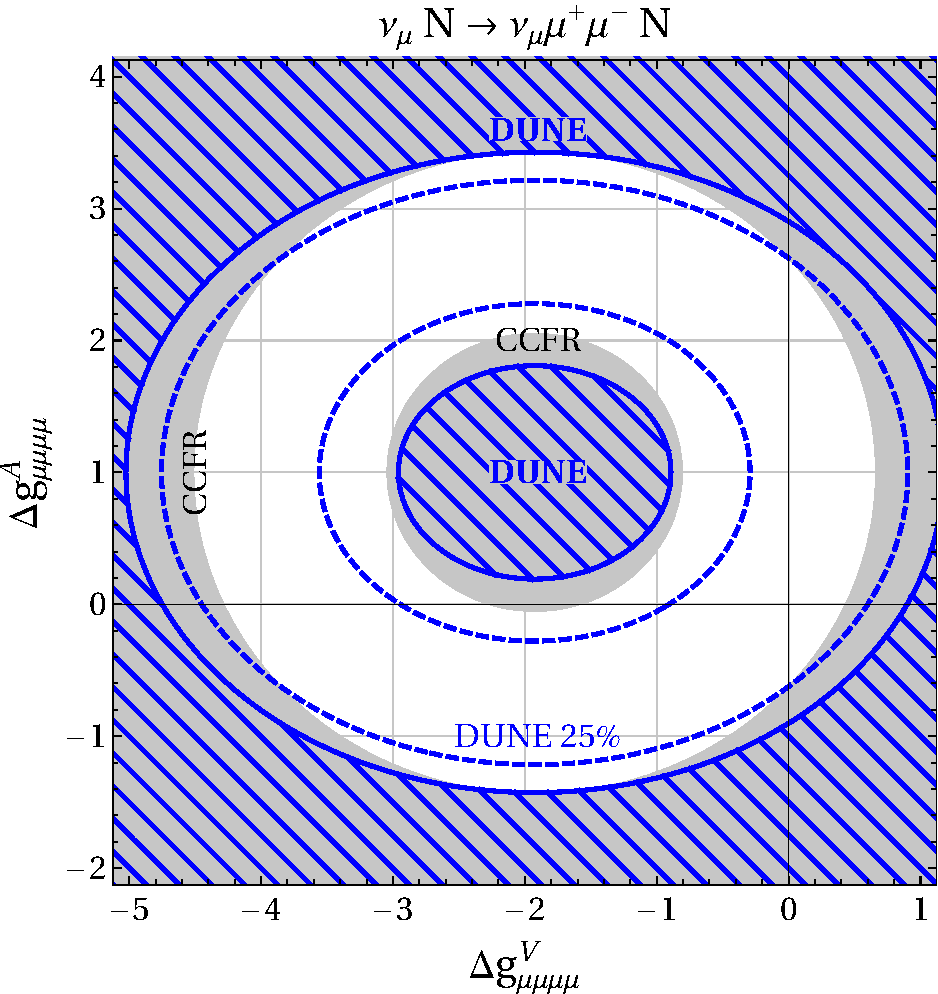
\includegraphics[width=0.4\textwidth]{graphics/model_independent_2.pdf}
\caption[$\nu_\mu N \to \nu_\mu \mu^+\mu^- N$ cross section at ND and (axial-)vector couplings of \numu{} to muons]
{Projected sensitivity (95\% \dword{cl}) of a measurement of the $\nu_\mu N \to \nu_\mu \mu^+\mu^- N$ cross section at the DUNE \dword{nd} to modifications of the vector and axial-vector couplings of muon-neutrinos to muons (blue hashed regions). The gray regions are excluded at 95\% \dword{cl} by existing measurements of the cross section by the CCFR collaboration. The intersection of the black lines indicates the \dword{sm} point.}
\label{fig:trident_gVgA}
\end{figure}
%%%%%%%%%%%%%%%%%%%%%%%%%%%%%%%%%%%%%%%%%%%%%%%%%%%%%%%%%%%%%%%

We consider a class of models that modify the trident cross section through the presence of an additional neutral gauge boson, $Z'$, that couples to neutrinos and charged leptons. A consistent way of introducing such a $Z'$ is to gauge an anomaly-free global symmetry of the \dword{sm}. Of particular interest is the $Z'$ that is based on gauging the difference of muon-number and tau-number, $L_\mu - L_\tau$~\cite{He:1990pn,He:1991qd}. Such a $Z'$ is relatively weakly constrained and can for example address the longstanding discrepancy between \dword{sm} prediction and measurement of the anomalous magnetic moment of the muon, $(g-2)_\mu$~\cite{Baek:2001kca,Harigaya:2013twa}. The $L_\mu - L_\tau$ $Z'$ has also been used in models to explain $B$ physics anomalies~\cite{Altmannshofer:2014cfa} and as a portal to \dword{dm}~\cite{Baek:2008nz,Altmannshofer:2016jzy}. The $\nu_\mu N \to \nu_\mu \mu^+\mu^- N$ trident process has been identified as important probe of gauged $L_\mu - L_\tau$ models over a broad range of $Z^\prime$ masses~\cite{Altmannshofer:2014cfa,Altmannshofer:2014pba}.

%%%%%%%%%%%%%%%%%%%%%%%%%%%%%%%%%%%%%%%%%%%%%%%%%%%%%%%%%%%%%%%
\begin{figure}[tb!] \centering
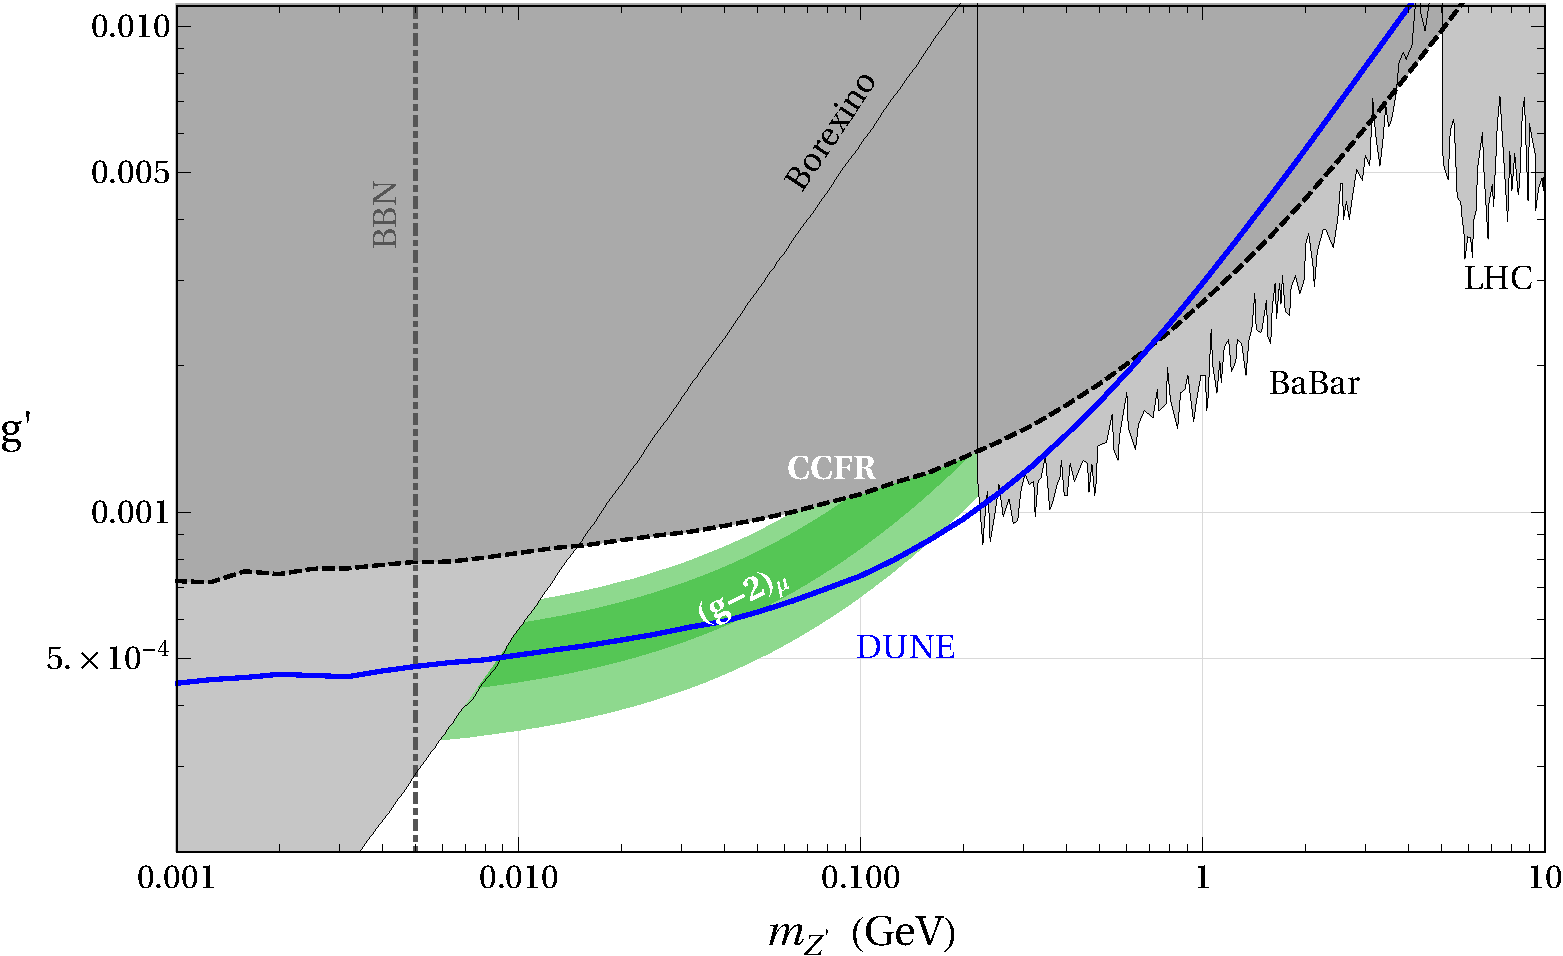
\includegraphics[width=0.75\textwidth]{LmuLtau_zoom.pdf}
\caption[Existing constraints and projected sensitivity in the $L_\mu - L_\tau$ parameter space]{Existing constraints and projected DUNE sensitivity in the $L_\mu - L_\tau$ parameter space. Shown in green is the region where the $(g-2)_\mu$ anomaly can be explained at the $2\sigma$ level. The parameter regions already excluded by existing constraints are shaded in gray and correspond to a CMS search for $pp \to \mu^+\mu^- Z' \to \mu^+\mu^-\mu^+\mu^-$~\cite{Sirunyan:2018nnz} (``LHC''), a BaBar search for $e^+e^- \to \mu^+\mu^- Z' \to \mu^+\mu^-\mu^+\mu^-$~\cite{TheBABAR:2016rlg} (``BaBar''), precision measurements of $Z \to \ell^+ \ell^-$ and $Z \to \nu\bar\nu$ couplings~\cite{ALEPH:2005ab,Altmannshofer:2014cfa} (``LEP''), a previous measurement of the trident cross section~\cite{Mishra:1991bv,Altmannshofer:2014pba} (``CCFR''), a measurement of the scattering rate of solar neutrinos on electrons~\cite{Bellini:2011rx,Harnik:2012ni,Agostini:2017ixy} (``Borexino''), and bounds from big bang nucleosynthesis~\cite{Ahlgren:2013wba,Kamada:2015era} (``BBN''). The DUNE sensitivity shown by the solid blue line assumes a measurement of the trident cross section with $40\%$ precision.}
\label{fig:LmuLtau}
\end{figure}
%%%%%%%%%%%%%%%%%%%%%%%%%%%%%%%%%%%%%%%%%%%%%%%%%%%%%%%%%%%%%%%

In Figure~\ref{fig:LmuLtau} we show the existing CCFR constraint on the model parameter space in the $m_{Z'}$ vs. $g'$ plane and compare it to the region of parameter space where the anomaly in $(g-2)_\mu = 2 a_\mu$ can be explained. The green region shows the $1\sigma$ and $2\sigma$ preferred parameter space corresponding to a shift $\Delta a_\mu = a_\mu^\text{exp}-a_\mu^\text{SM} = (2.71 \pm 0.73) \times 10^{-9}$~\cite{Keshavarzi:2018mgv}.
Shown are in addition constraints from LHC searches for the $Z'$ in the $pp \to \mu^+\mu^- Z' \to \mu^+\mu^-\mu^+\mu^-$ process~\cite{Sirunyan:2018nnz} (see also~\cite{Altmannshofer:2014pba}), direct searches for the $Z'$ at BaBar using the $e^+e^- \to \mu^+\mu^- Z' \to \mu^+\mu^-\mu^+\mu^-$ process~\cite{TheBABAR:2016rlg}, and constraints from LEP precision measurements of leptonic $Z$ couplings~\cite{ALEPH:2005ab,Altmannshofer:2014cfa}.  
Also a Borexino bound on non-standard contributions to neutrino-electron scattering~\cite{Harnik:2012ni,Bellini:2011rx,Agostini:2017ixy} has been used to constrain the $L_\mu - L_\tau$ gauge boson~\cite{Kamada:2015era,Araki:2015mya,Kamada:2018zxi}. Our reproduction of the Borexino constraint is shown. 
For very light $Z'$ masses of $O$(few MeV) and below, strong constraints from measurements of the effective number of relativistic degrees of freedom during big bang nucleosynthesis (BBN) apply~\cite{Ahlgren:2013wba,Kamada:2015era}.
Taking into account all relevant constraints, parameter space to explain $(g-2)_\mu$ is left below the di-muon threshold $m_{Z'} \lesssim 210$~MeV.

%%% NEUTRINO TRIDENTS %%%%%%%%%%%%%%%%%%%%%%%%%%%%%%%



%%%%%%%%%%%%%%%%%%%%%%%%%%%%%%%%%%%%%%%%
\section{Dark Matter Probes}\label{sec:DM}
Dark matter (\dword{dm}) is a crucial ingredient to understand the cosmological history of the universe, and the most up-to-date measurements suggests the existence of \dword{dm} with an abundance of 27\%~\cite{Aghanim:2018eyx}. 
In light of this situation, a tremendous amount of experimental effort has gone into %been made in 
the search for \dword{dm}-induced signatures, for example, \dword{dm} direct and indirect detections and collider searches. However, no ``smoking-gun'' signals have been discovered thus far while more parameter space in relevant \dword{dm} models is simply ruled out. %\\ 
It is noteworthy that most conventional \dword{dm} search strategies are designed to be sensitive to signals from the \dword{wimp}, one of the well-motivated \dword{dm} candidates, whose mass range is from a few GeV to tens of TeV. 
The null observation of \dword{dm} via non-gravitational interactions actually motivates unconventional or alternative \dword{dm} search schemes. 
One such possibility is %to look 
a search for experimental signatures induced by boosted, hence relativistic, \dword{dm} for which %the mass range smaller than the weak scale is often motivated. 
a mass range smaller than that of the weak scale is often motivated. 

One of the possible ways to produce and then detect relativistic \dword{dm} particles can be through accelerator experiments, 
for example, neutrino beam experiments~\cite{Alexander:2016aln, Battaglieri:2017aum, LoSecco:1980nf, Acciarri:2015uup}. 
By construction, large signal statistics is expected so that this sort of search strategy can allow for significant
sensitivity to \dword{dm}-induced signals despite the feeble interaction of \dword{dm} with \dword{sm} particles. %\\
DUNE will perform a signal search in the relativistic scattering of \dword{ldm} at the \dword{nd}, as it is close enough to the beam source to sample a substantial level of \dword{dm} flux, assuming that \dword{dm} is produced.

%Alternatively, \dword{bdm} particles can be created in the universe today under non-minimal dark-sector scenarios~\cite{Agashe:2014yua,Belanger:2011ww}, and reach terrestrial detectors.
Alternatively, it is possible that \dword{bdm} particles are created in the universe under non-minimal dark-sector scenarios~\cite{Agashe:2014yua,
Belanger:2011ww}, and can reach terrestrial detectors. 
For example, one can imagine a two-component \dword{dm} scenario in which a lighter component is usually a subdominant relic with direct coupling to \dword{sm} particles, while the heavier is the cosmological \dword{dm} that pair-annihilates directly to a lighter \dword{dm} pair, not to \dword{sm} particles. Other mechanisms such as semi-annihilation in which a \dword{dm} particle pair-annihilates to a lighter \dword{dm} particle and a dark sector particle that may decay away are also possible~\cite{Carlson:1992fn, Hochberg:2014dra,Huang:2013xfa,Berger:2014sqa,Kong:2014mia}.
In typical cases, the \dword{bdm} flux is not large and thus large-volume neutrino detectors are desirable %better motivated than small-size detectors 
to overcome the challenge in statistics (for an  exception, see~\cite{Cherry:2015oca, Cui:2017ytb}).

Indeed, a (full-fledged) DUNE \dword{fd} with a fiducial mass of \fdfiducialmass and quality detector performance is expected to possess competitive sensitivity to \dword{bdm} signals from various sources in the current universe such as the galactic halo~\cite{Agashe:2014yua,
Alhazmi:2016qcs,Kim:2016zjx,Giudice:2017zke,Chatterjee:2018mej,Kim:2018veo}, the sun~\cite{Huang:2013xfa,Berger:2014sqa,Kong:2014mia,Kim:2018veo}, and dwarf spheroidal galaxies~\cite{Necib:2016aez}.
Furthermore, the \dword{protodune} detectors %, prototypes for the DUNE \dword{fd}, 
are operational, and we anticipate preliminary studies with their cosmic data. Interactions of \dword{bdm} with electrons~\cite{Agashe:2014yua} 
and with hadrons (protons)~\cite{Berger:2014sqa}, were investigated for Cherenkov detectors, such as \superk, which recently published a dedicated search for \dword{bdm} in the electron channel~\cite{Kachulis:2017nci}. However, in such detectors the \dword{bdm} signal rate is shown to often be significantly attenuated due to Cherenkov threshold, in particular for hadronic channels.  \lar detectors, such as DUNE's, have the potential to greatly improve the sensitivity for \dword{bdm} compared to Cherenkov detectors. This is due to improved particle identification techniques, as well as a significantly lower energy threshold for proton detection. Earlier studies have shown an improvement with DUNE for\dword{bdm}-electron interaction~\cite{Necib:2016aez}.

%%%%%%%%%%%%%%%%%%%%%%%%%
\subsection{Benchmark Dark Matter Models}
\label{sec:model}


The benchmark ``\dword{dm} models'' defined in this section describe only couplings of dark-sector states including \dword{ldm} particles.
%(denoted by $\chi_1$). 
We consider two example models: i) a vector portal-type scenario where a (massive) dark-sector photon $V$ mixes with the \dword{sm} photon and ii) a leptophobic $Z'$ scenario.
The former is used in Sections~\ref{sec:ND} and \ref{sec:FD}, while the latter features in Section~\ref{sec:FDsun}.
%First of all, we describe a vector portal-type scenario where a (massive) dark-sector photon $V$ mixes with the \dword{sm} photon. 
\dword{dm} and other dark-sector particles are assumed to be fermionic for convenience.

\paragraph{Benchmark Model i)}
%\dword{dm} and other dark-sector particles are assumed to be fermionic for convenience. 

The relevant interaction Lagrangian is given by
\bea
\mathcal{L}_{\rm int} \supset -\frac{\epsilon}{2}V_{\mu\nu}F^{\mu\nu}+g_{11} \bar{\chi}_1\gamma^\mu \chi_1 V_\mu+g_{12} \bar{\chi}_2\gamma^\mu \chi_1 V_\mu +h.c.\,, 
\label{eq:lagrangian}
\eea
where $V^{\mu\nu}$ and $F^{\mu\nu}$ are the field strength tensors for the dark-sector photon and the \dword{sm} photon, respectively. 
Here we have introduced the kinetic mixing parameter $\epsilon$, while $g_{11}$ and $g_{12}$ parameterize the interaction strengths for flavor-conserving (second operator) and flavor-changing (third operator) couplings, respectively.  
Here $\chi_1$ and $\chi_2$ denote a dark matter particle and a heavier, \textit{un}stable dark-sector state, respectively (i.e., $m_{\chi_2}>m_{\chi_1}$), and the third term allows (boosted) $\chi_1$ to up-scatter to this $\chi_2$ (i.e., an ``inelastic'' scattering process).

%We remark that o
This model introduces five new free parameters that may be varied for our sensitivity analysis: dark photon mass $m_V$, \dword{dm} mass $m_{\chi_1}$, heavier dark-sector state mass $m_{\chi_2}$, kinetic mixing parameter $\epsilon$, dark-sector diagonal coupling $\alpha_{11} =g_{11}^2/(4\pi)$, and dark-sector off-diagonal coupling $\alpha_{12} =g_{12}^2/(4\pi)$. 
We shall perform our analyses with some of the parameters fixed to certain values for illustration.

\paragraph{Benchmark Model ii)}
This model employs a leptophobic $Z^\prime$ mediator for interactions with the nucleons. The interaction lagrangian for this model is
\bea
\mathcal{L}_{\rm int} \supset - g_{\rm Z^\prime} \sum_f Z^\prime_\mu \bar{q}_f \gamma^\mu \gamma^5 q_f - g_{\rm Z^\prime} Z^\prime_\mu \bar{\chi} \gamma^\mu \gamma^5 \chi - Q_\psi g_{\rm Z^\prime} Z^\prime_\mu \bar{\psi} \gamma^\mu \gamma^5 \psi. 
\label{eq:zprimelag}
\eea
Here, all couplings are taken to be axial. $f$ denotes the quark flavors in the \dword{sm} sector. The dark matter states are denoted by $\chi$ and $\psi$ with $m_\chi < m_\psi$. The coupling $g_{\rm Z^\prime}$ and the masses of the dark matter states are free parameters. $Q_\psi$ is taken to be less than 1 and determines the abundance of dark matter in the universe. The hadronic interaction model study presented here is complementary to and has different phenomenology compared to others such as Benchmark Model i).
The study of this benchmark model and the result are discussed in Section~\ref{sec:FDsun}.

%%%%%%%%%%%%%%%%%%%%%%%%%
\subsection{Search for Low-Mass Dark Mater at the Near Detector} \label{sec:ND}
\subsubsection{Dark Matter Production and Detection}
\label{sec:DMProd}

Here, we focus on Benchmark Model i) from Eq.~(\ref{eq:lagrangian}), specifically where only one \dword{dm} particle $\chi \equiv \chi_1$ exists. We also define the dark fine structure constant $\alpha_D \equiv g_{11}^2/4\pi$. We assume that $\chi$ is a fermionic thermal relic -- in this case, the \dword{dm}/dark photon masses and couplings will provide a target for which the relic abundance matches the observed abundance in the universe. Here, the largest flux of dark photons $V$ and \dword{dm} to reach the DUNE \dword{nd} will come from the decays of light pseudoscalar mesons (specifically $\pi^0$ and $\eta$ mesons) that are produced in the DUNE target, as well as proton bremsstrahlung processes $p + p \to p + p + V$.
For the entirety of this analysis, we will fix $\alpha_D = 0.5$ and assume that the DM mass $M_{\chi}$ is lighter than half the mass of a pseudoscalar meson $\mathfrak{m}$ that is produced in the DUNE target. In this scenario, $\chi$  is produced via two decays, those of on-shell $V$ and those of off-shell $V$. This production is depicted in Figure~\ref{fig:dm_prod}. 
%\KJK{Meson production needs to replace the left panel.}.

The flux of \dword{dm} produced via meson decays -- via on-shell $V$ -- may be estimated by\footnote{See Ref.~\cite{DeRomeri:2019kic} for a complete derivation of these expressions, including those for meson decays via off-shell $V$.}
\begin{equation}
    N_\chi = 2 N_\mathrm{POT} c_\mathfrak{m} \mathrm{Br}(\mathfrak{m}\to \gamma\gamma) \left[ 2 \varepsilon^2 \left(1 - \frac{M_{V}^2}{m_\mathrm{m}^2}\right)^3\right] \mathrm{Br}(V \to \chi\bar{\chi}) g(M_\chi, M_{V}),
\end{equation}
where $N_\mathrm{POT}$ is the number of protons on target delivered by the beam, $c_\mathfrak{m}$ is the average number of meson $\mathfrak{m}$ produced per POT, the term in braces is the relative branching fraction of $\mathfrak{m} \to \gamma V$ relative to $\gamma\gamma$, and $g(x, y)$ characterizes the geometrical acceptance fraction of \dword{dm} reaching the DUNE \dword{nd}. $g(x, y)$ is determined given model parameters using Monte Carlo techniques. For the range of dark photon and \dword{dm} masses in which DUNE will set a competitive limit, the \dword{dm} flux due to meson decays will dominate over the flux due to proton bremsstrahlung. Considering \dword{dm} masses in the $\sim$1-300 MeV range, this will require production via the $\pi^0$ and $\eta$ mesons. Our simulations using {\sc Pythia} determine that $c_{\pi^0} \approx 4.5$ and $c_\eta \approx 0.5$.

\begin{figure}[t]
\centering
 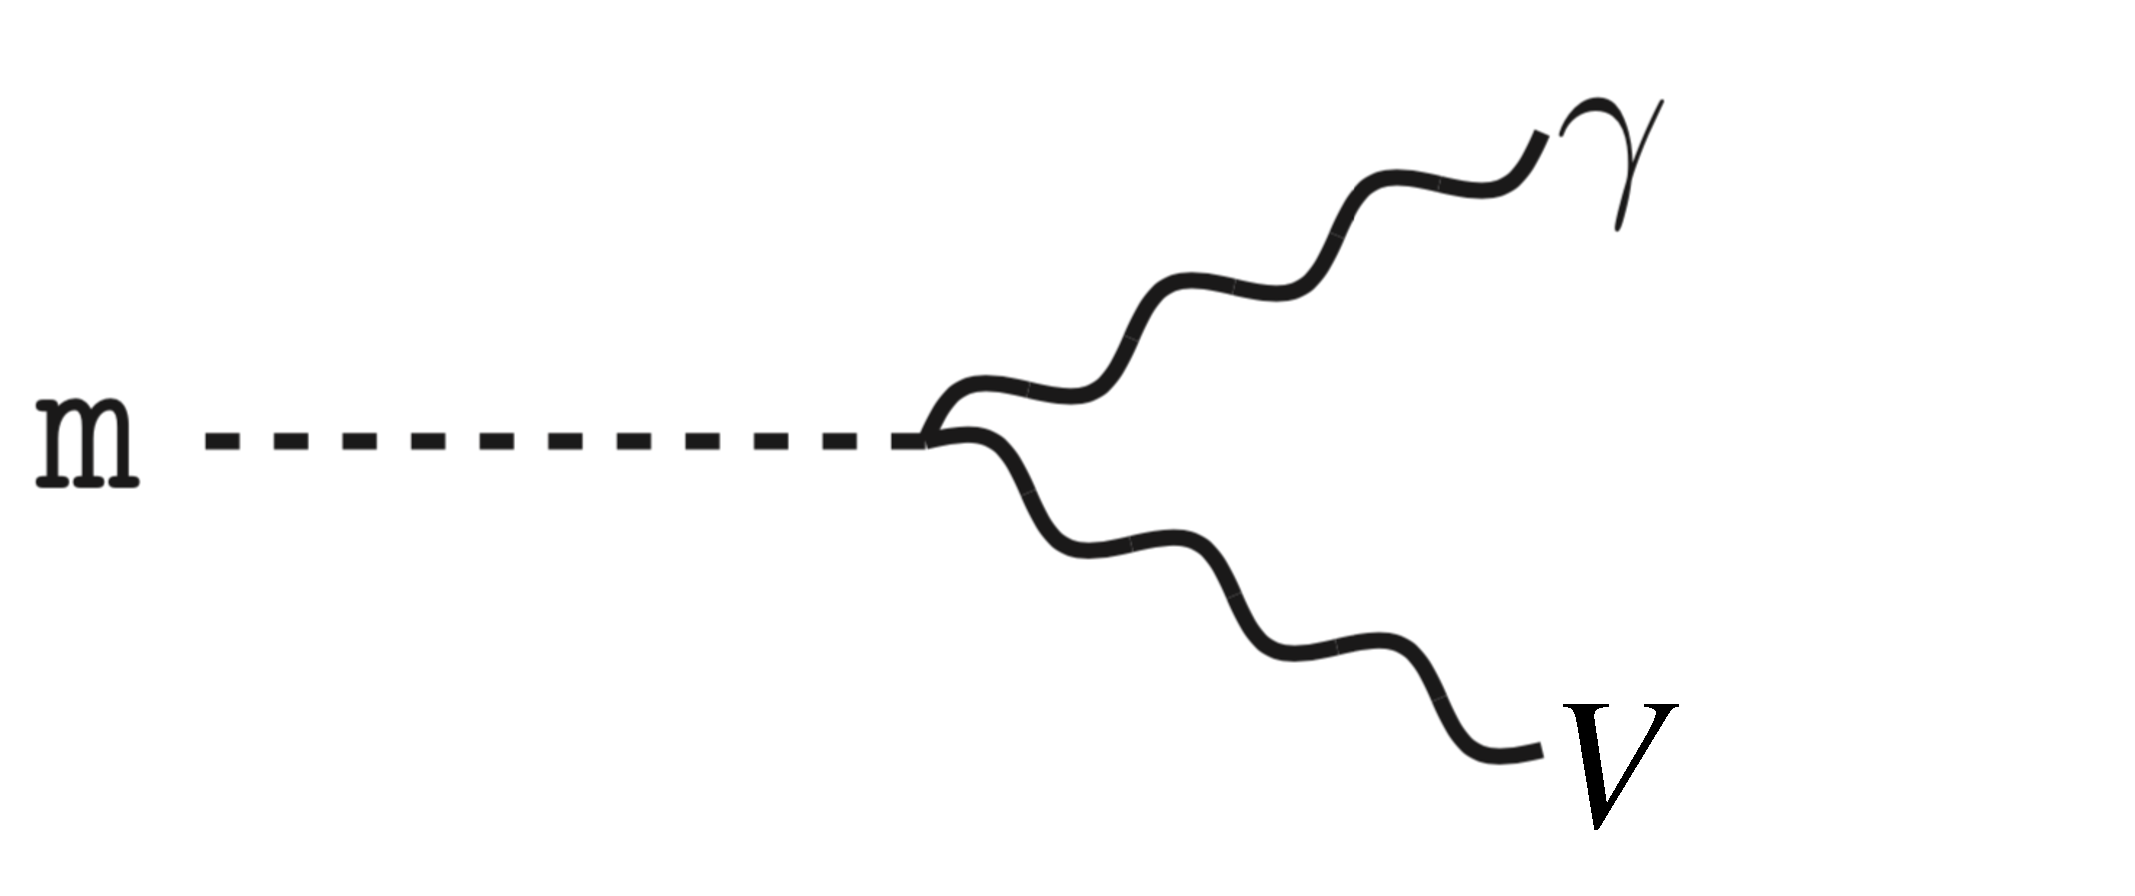
\includegraphics[width=0.30\linewidth]{MesonDecay_2Body.pdf}
    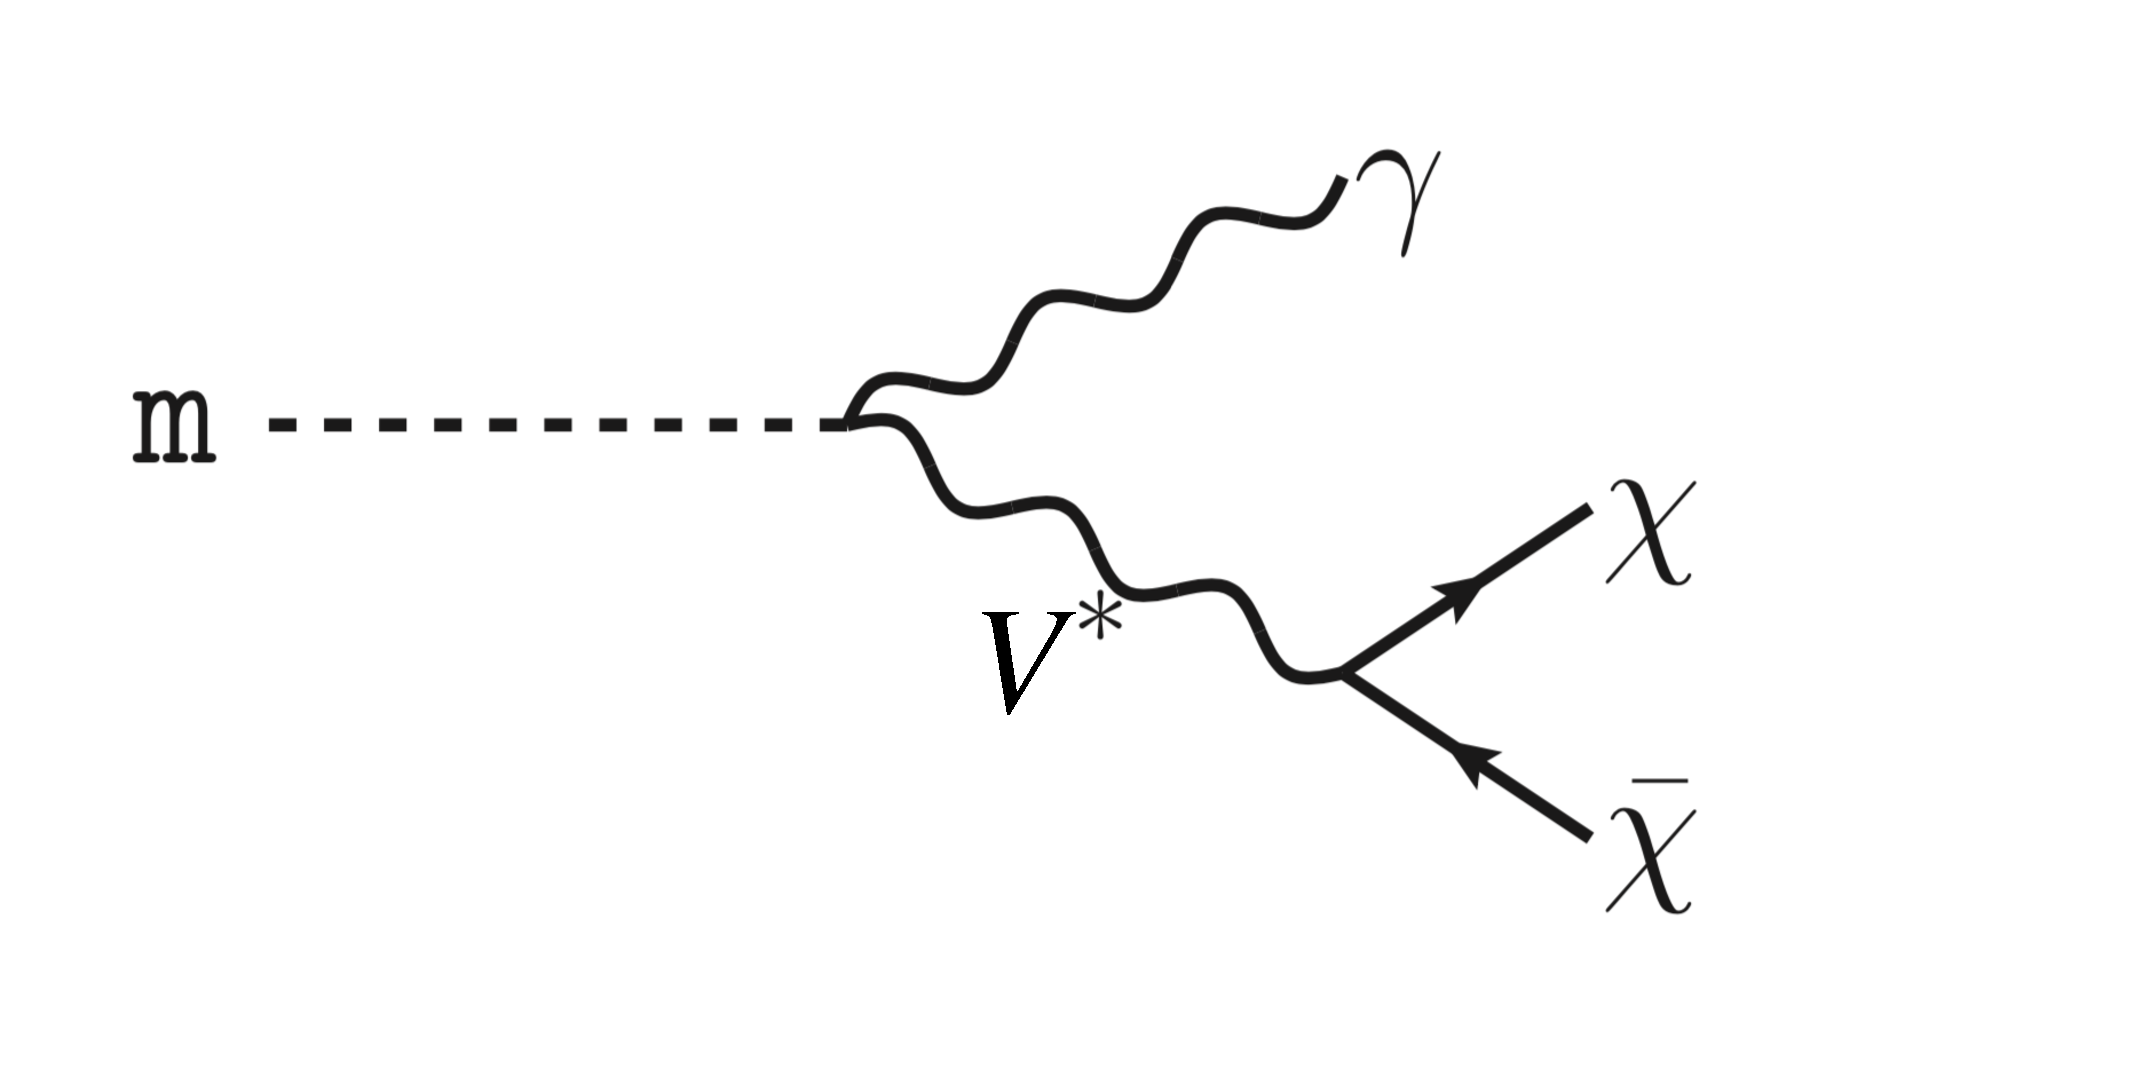
\includegraphics[width=0.30\linewidth]{MesonDecay.pdf}
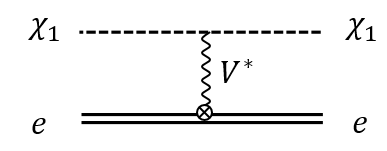
\includegraphics[width=0.30\textwidth]{graphics/DM_detect.png}
\caption[DM production via meson decays and DM-e$^-$ elastic scattering]{ 
Production of fermionic \dword{dm} via two-body pseudoscalar meson decay $\mathfrak{m} \to \gamma V$, when $M_{V} < m_\mathfrak{m}$ (left) or via three-body decay $\mathfrak{m} \to \gamma \chi \overline{\chi}$ (center) and \dword{dm}-electron elastic scattering (right panel).}
\label{fig:dm_prod}
\end{figure}

If the \dword{dm} reaches the near detector, it may scatter elastically off nucleons or electrons in the detector, via a $t$-channel dark photon. Due to its smaller backgrounds, we focus on scattering off electrons, depicted in the right panel of Figure~\ref{fig:dm_prod}. The differential cross section of this scattering, as a function of the recoil energy of the electron $E_e$, is
\begin{equation}
\frac{d\sigma_{{\chi}e}}{dE_{e}} 
= 4\pi \epsilon^{2}\alpha_D\alpha_{EM} \frac{2m_{e}E_{\chi}^{2} - (2m_{e}E_{\chi} + m_{\chi}^{2})(E_e-m_{e})}{(E_e^{2}-m_{\chi}^{2})(m_{V}^{2}+2m_{e}E_{e}-2m_{e}^{2})^{2}}\,,
\end{equation}
where $E_{\chi}$ is the incoming \dword{dm} $\chi$ energy. The signal is an event with only one recoil electron in the final state. We may use the scattering angle and energy of the electron to distinguish between signal and background (discussed in the following) events.

\subsubsection{Background Considerations}
 The background to the process shown in the right panel of Figure~\ref{fig:dm_prod} consists of any processes involving an electron recoil. As the \dword{nd} is located near the surface, background events, in general, can be induced by cosmic rays as well as by neutrinos generated from the beam. Since majority of cosmic-induced, however, will be vetoed by triggers and timing information, the dominant background will be from neutrinos coming in the DUNE beam.

The two neutrino-related backgrounds are $\nu_\mu -e^-$ scattering, which looks nearly identical to the signal, and $\nu_e$ CCQE scattering, which does not. The latter has a much larger rate ($\sim$ 10 times higher) than the former, however, we expect that using the kinematical variable $E_e \theta_e^2$ of the final state, where $\theta_e$ is the direction of the outgoing electron relative to the beam direction, will allow the $\nu_e$ CCQE background to be vetoed effectively.

While spectral information regarding $E_e$ could allow a search to distinguish between $\chi e$ and $\nu_\mu e$ scattering, we expect that uncertainties in the $\nu_\mu$ flux (both in terms of overall normalization and shape as a function of neutrino energy) will make such an analysis very complicated. For this reason, we include a normalization uncertainty of $10\%$ on the expected background rate and perform a counting analysis. Studies are ongoing to determine how such an analysis may be improved.

For this analysis we have assumed $3.5$ years of data collection each in neutrino and antineutrino modes, analyzing events that occur within the fiducial volume of the DUNE near detector. We compare results assuming either all data is collected with the ND on-axis, or data collection is divided equally among all off-axis positions, $0.7$ yr at each position  $i$, between $0$ and $24$ m transverse to the beam direction (in steps of 6 meters).
We assume three sources of uncertainty: statistical, correlated systematic, and an uncorrelated systematic in each bin. 
For a correlated systematic uncertainty, we include a nuisance parameter $A$ that modifies the number of neutrino-related background events in all bins -- an overall normalization uncertainty across all off-axis locations. 
We further include an additional term in our test statistic for $A$, a  Gaussian probability with width $\sigma_A = 10\%$. 
We also include an uncorrelated uncertainty in each bin, which we assume to be much narrower than $\sigma_A$. 
We assume this uncertainty to be parameterized by a Gaussian with width $\sigma_{f_i} = 1\%$. 
After marginalizing over the corresponding uncorrelated nuisance parameters, the test statistic reads
\begin{eqnarray}\label{eq:chisqfull}
-2\Delta \mathcal{L} = \sum_i \frac{r_i^m\left( \left(\frac{\varepsilon}{\varepsilon_0}\right)^4 N_i^\chi + (A-1)N_i^\nu\right)^2}{A\left(N_i^\nu + (\sigma_{f_i} N_i^\nu)^2 \right)} + \frac{\left(A-1\right)^2}{\sigma_A^2}.
\end{eqnarray}



In Eq.~(\ref{eq:chisqfull}), $N_i^\chi$ is the number of \dword{dm} scattering events, calculated assuming $\varepsilon$ is equal to some reference value $\varepsilon_0 \ll 1$. $N_i^\nu$ is the number of $\nu_\mu e^-$ scattering events expected in detector position $i$, and $r_i^m$ is the number of years of data collection in detector position $i$ during beam mode $m$ (neutrino or antineutrino mode). If data are only collected on-axis, then this test statistic will be dominated by the systematic uncertainty associated with $\sigma_A$. If on- and off-axis measurements are combined, then the resulting sensitivity will improve significantly.

\subsubsection{Sensitivity Calculation and Results}

We compute the expected DUNE sensitivity assuming all data collected with the ND on-axis (DUNE On-axis) or equal times at each ND off-axis position (DUNE-PRISM). We present results in terms of the \dword{dm} or dark photon mass and the parameter $Y$, where
\begin{equation}
Y \equiv \varepsilon^2 \alpha_D \left(\frac{M_\chi}{M_V}\right)^4.    
\end{equation}
Assuming $M_V \gg M_\chi$, this parameter determines the relic abundance of \dword{dm} in the universe today, and sets a theoretical goal in terms of sensitivity reach. We present the 90\% CL sensitivity reach of the DUNE \dword{nd} in Figure~\ref{fig:chisq}. 
We assume $\alpha_D = 0.5$ in our simulations and we display the results fixing $M_V = 3M_\chi$ (left panel) and $M_\chi = 20$ MeV (right panel).
We also compare the sensitivity reach of this analysis with other existing experiments, shown as grey shaded regions. We further show for comparison the sensitivity curve expected for a proposed dedicated experiment to search for \dword{ldm}, LDMX-Phase I~\cite{Akesson:2018vlm} (solid blue).

 \begin{figure}[t]
 \centering
 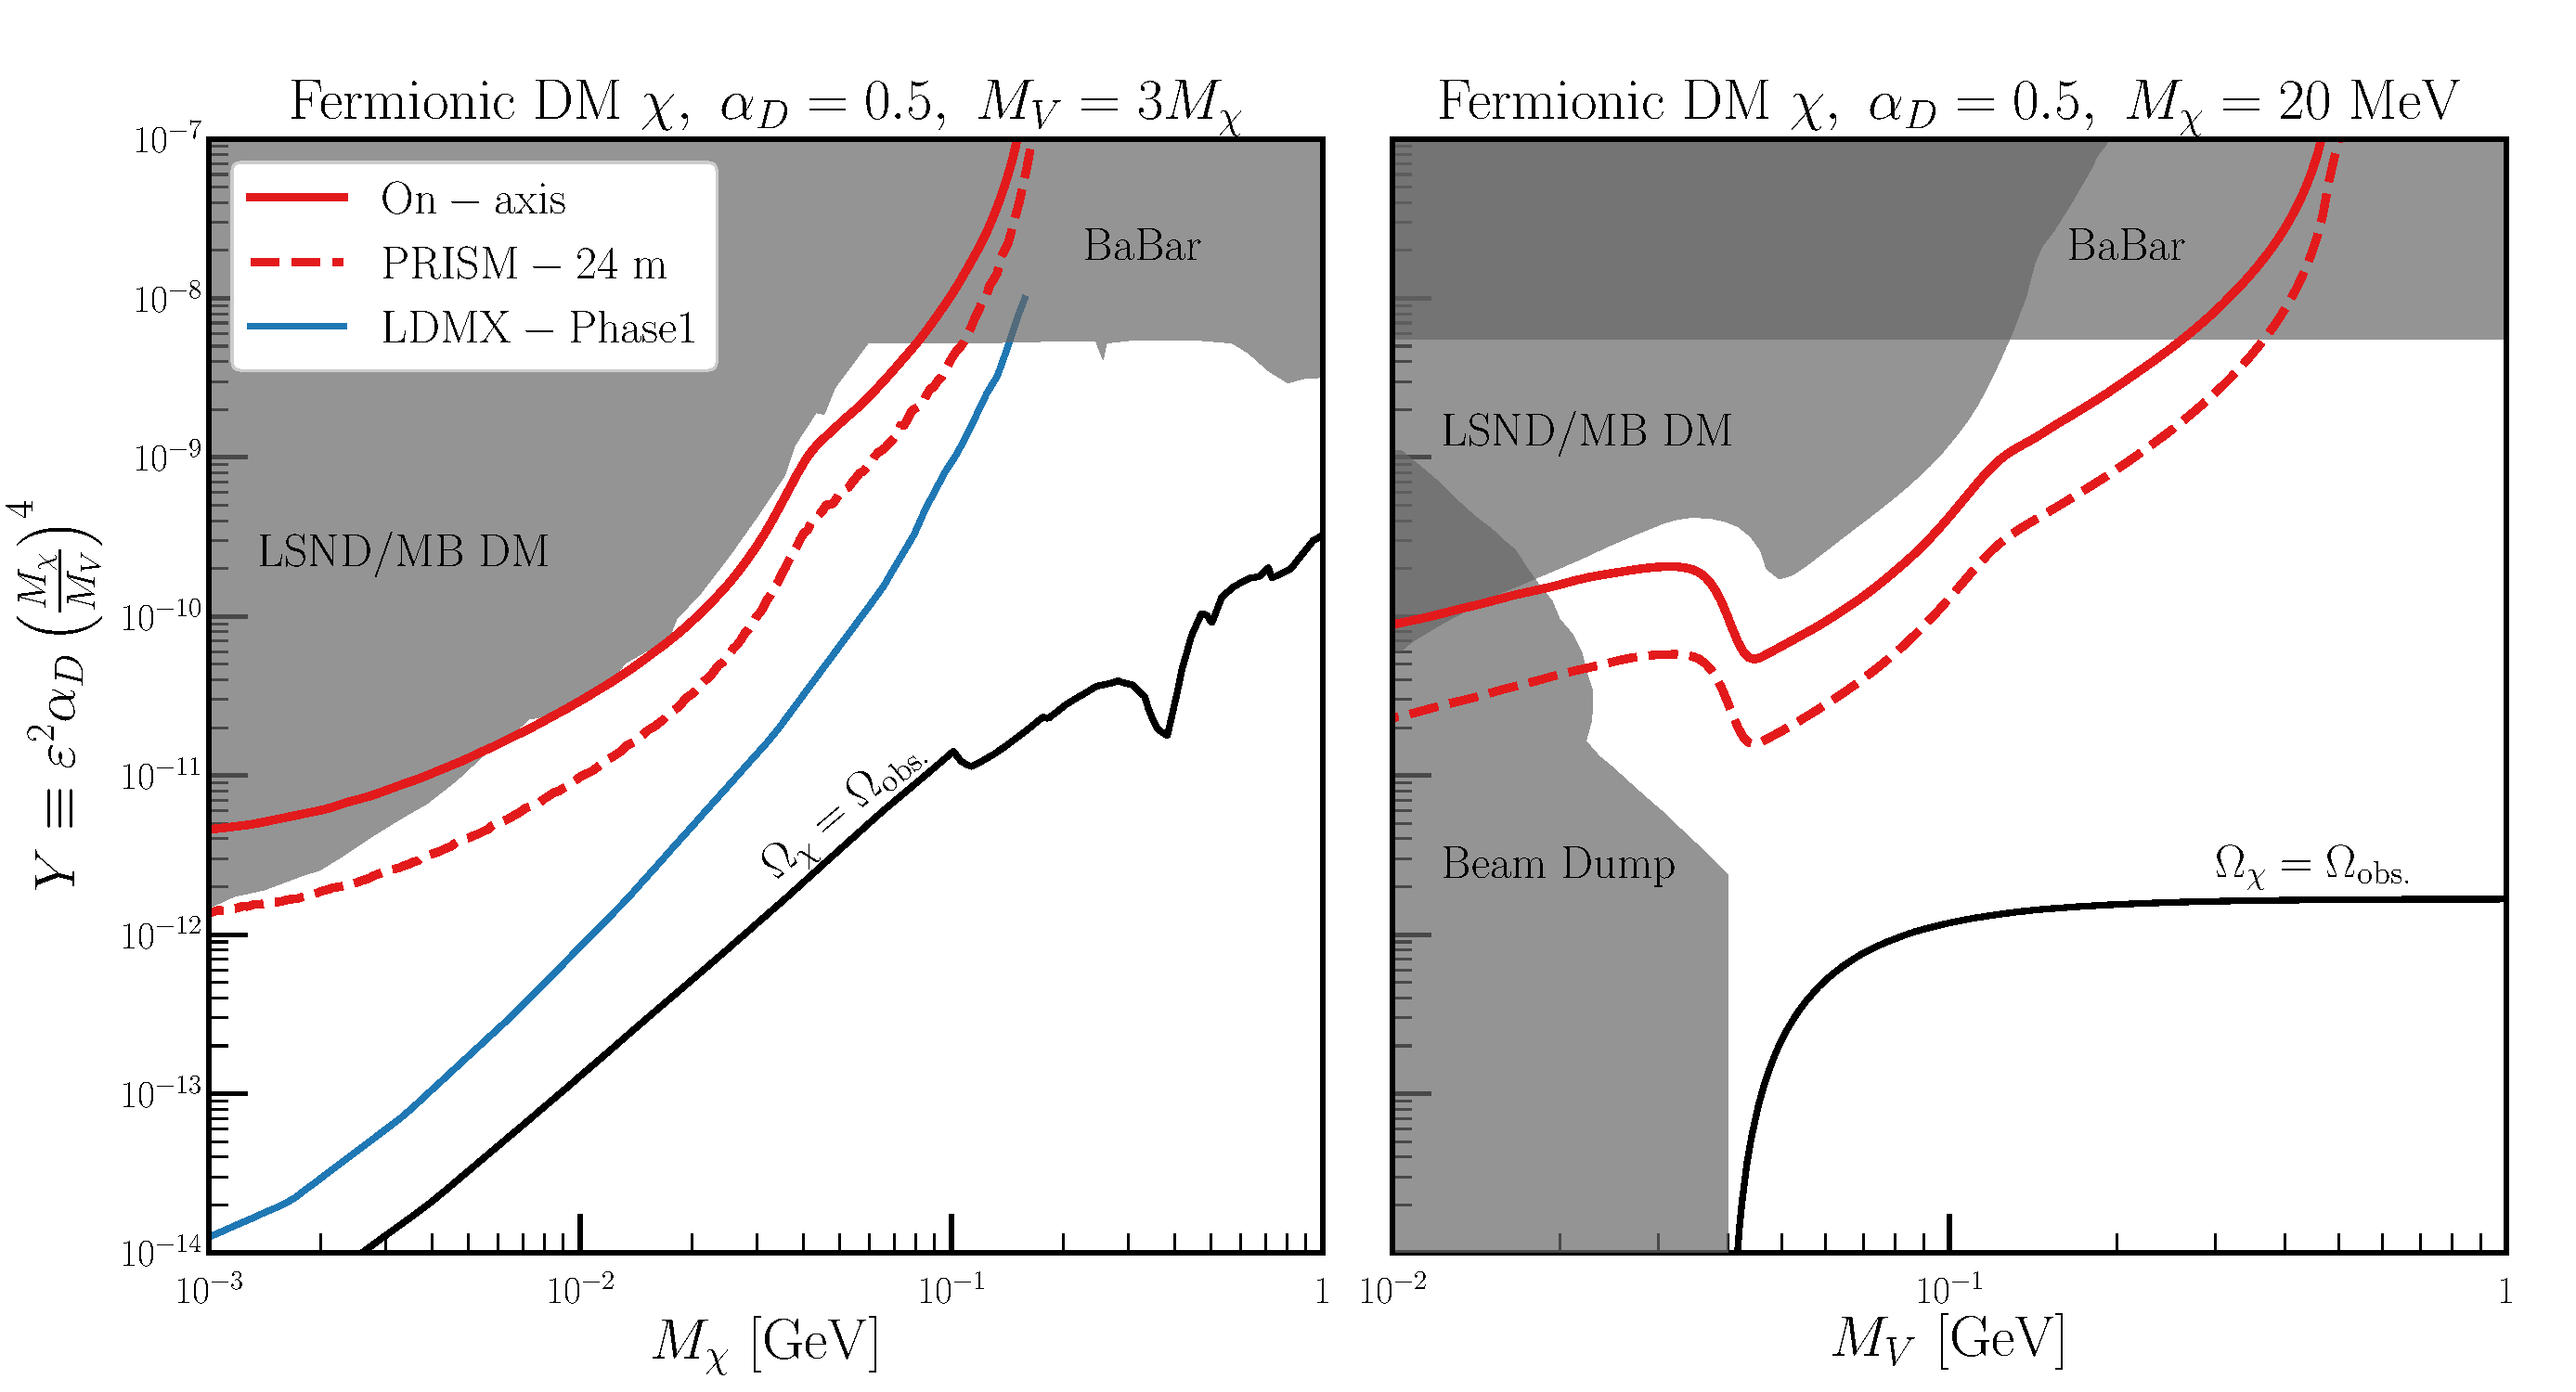
\includegraphics[width=\linewidth]{graphics/LDM_Sensitivity.pdf}
 \caption[90$\%$ \dword{cl} limit for Y as a function of $m_{\chi}$ at the ND]{\label{fig:chisq} Expected DUNE On-axis (solid red) and PRISM (dashed red) sensitivity using $\chi e^- \to \chi e^-$ scattering. We assume $\alpha_D = 0.5$ in both panels, and $M_V = 3M_\chi$ ($M_\chi = 20$ MeV) in the left (right) panel, respectively. Existing constraints are shown in grey, and the relic density target is shown as a black line. We also show for comparison the sensitivity curve expected for LDMX-Phase I (solid blue)~\cite{Akesson:2018vlm}.
 }
 \end{figure}

 From our estimates, we see that DUNE can significantly improve the constraints from LSND~\cite{deNiverville:2018dbu} and the MiniBooNE-DM search~\cite{Aguilar-Arevalo:2018wea}, as well as BaBar~\cite{Lees:2017lec} if $M_V \lesssim 200$ MeV. We also show limits in the right panel from beam-dump experiments (where the dark photon is assumed to decay visibly if $M_V < 2 M_\chi$)~\cite{Davier:1989wz,Batley:2015lha,Bjorken:1988as,Riordan:1987aw,Bjorken:2009mm,Bross:1989mp}, as well as the lower limits obtained from matching the thermal relic abundance of $\chi$ with the observed one (black).

The features in the sensitivity curve in the right panel can be understood by looking at the DM production mechanism.
For a fixed $\chi$ mass, as $M_V$ grows, the DM production goes from off-shell to on-shell and back to off-shell. The first transition explains the strong feature near $M_V=2M_\chi = 40$~MeV, while the second is the source for the slight kink around $M_V=m_{\pi^0}$ (which appears also in the left panel).





%%%%%%%%%%%%%%%%%%%%%%%%%
\subsection{Inelastic Boosted Dark Matter Search at the DUNE FD 
%and \dword{protodune}
\label{sec:FD}}

\subsubsection{\dshort{bdm} Flux from the Galactic Halo \label{sec:flux}}

As we mentioned in Section~\ref{phys:bsm:execsumm}, %the Introduction, 
we look at an annihilating two-component \dword{dm} scenario~\cite{Belanger:2011ww} in this study. 
The heavier \dword{dm} (denoted $\chi_0$) plays a role of cosmological \dword{dm} and pair-annihilates to a pair of lighter \dword{dm} particles (denoted $\chi_1$) in the universe today. 
The expected flux near the Earth is given by~\cite{Agashe:2014yua,
Giudice:2017zke, Kim:2018veo}
\bea 
\mathcal{F}_1= & 1.6 \times 10^{-6} {\rm cm}^{-2}{\rm s}^{-1}\times \left( \frac{\langle \sigma v\rangle_{0\rightarrow 1}}{5\times 10^{-26}{\rm cm}^3{\rm s}^{-1}}\right) 
 \times \left( \frac{10\, {\rm GeV}}{m_{\chi_0}}\right)^2\,,
\label{eq:flux}
\eea
where $m_{\chi_0}$ is the mass of $\chi_0$ and $\langle \sigma v\rangle_{0\rightarrow 1}$ stands for the velocity-averaged annihilation cross section of $\chi_0\bar{\chi}_0 \to \chi_1\bar{\chi}_1$ in the current universe.
To evaluate the reference value shown as the first prefactor, we take $m_{\chi_0} = 10$ GeV and $\langle \sigma v\rangle_{0\rightarrow 1}=5\times 10^{-26}{\rm cm}^3{\rm s}^{-1}$, the latter of which is consistent with the current observation of \dword{dm} relic density assuming $\chi_0$ and its anti-particle $\bar{\chi}_0$ are distinguishable. 
To integrate all relevant contributions over the entire galaxy, we assume the Navarro-Frenk-White (NFW) \dword{dm} halo profile~\cite{Navarro:1995iw, Navarro:1996gj}.
In this section we assume the \dword{bdm} flux with a $m_{\chi_0}$ dependence given by eq.~(\ref{eq:flux}) for the phenomenological analysis. 


\subsubsection{Experimental Signatures}

The \dword{bdm} that is created, e.g., at the galactic center, reaches the DUNE \dword{fd} 
%and \dword{protodune} 
detectors and scatters off either electrons or protons energetically. 
In this study, we focus on electron scattering signatures for illustration, under Benchmark Model i) defined in eq.~\eqref{eq:lagrangian}. 
The overall process is summarized as follows:
\bea 
\chi_1 + e^- \to e^- + \chi_2 (\to \chi_1 + V^{(*)} \to \chi_1 + e^+ +e^-)\,,
\eea
and a diagrammatic description is shown in Figure~\ref{fig:sig} where %detector-visible 
particles visible by the detector are circled in blue. %enclosed by a blue circle. 
%Therefore, i
In the final state, there exist three visible particles that usually leave sizable ($e$-like) tracks in the %DUNE and \dword{protodune} 
detectors.  
Note that we can replace $e^-$ in the left-hand side and the first $e^-$ in the right-hand side of the above process to $p$ for the $p$-scattering case.
In the basic model, eq.~\eqref{eq:lagrangian}, and given the source of \dword{bdm} at the galactic center,  the primary signature is quasi-elastic proton recoiling~\cite{pscattering} in this case.

\begin{figure}[t]
\centering
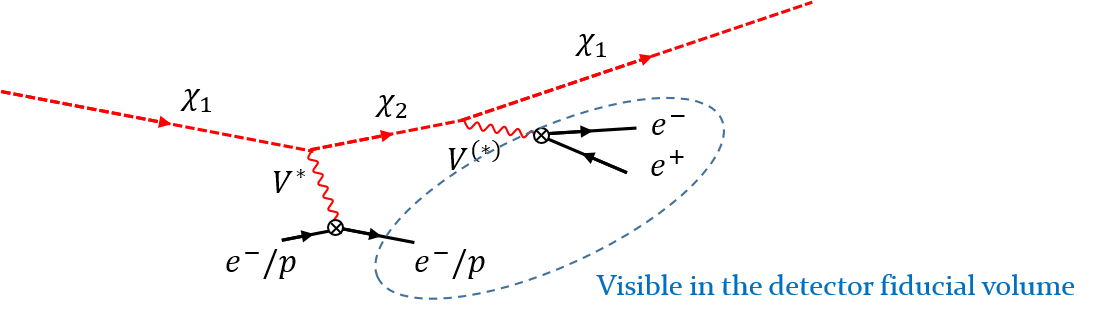
\includegraphics[width=9cm]{signature}
\caption{\label{fig:sig} The inelastic BDM signal under consideration.}
\end{figure}

\subsubsection{Background Estimation}

As we have identified a possible $i$\dword{bdm} signature, we are now in a position to discuss potential \dword{sm} background events. 



%When it comes to the 
For the DUNE \dwords{detmodule} located $\sim 1480$ m deep underground, the cosmic-induced background discussed earlier is not an issue. 
The most plausible scenario for background production is the creation of multiple pions that subsequently decay to electrons, positrons, and neutrinos. 
Relevant channels are the resonance production and/or \dword{dis} by the \dword{cc} $\nu_e$ or $\bar \nu_e$ scattering with a nucleon in the \lar target.
Summing up all the resonance production and \dword{dis} events that are not only induced by $\nu_e$ or $\bar \nu_e$ 
%whose energy is larger than 1 GeV, 
but relevant to production of a few pions, we find that the total number of multi-pion production events is at most $\sim 12$ kt$^{-1}$yr$^{-1}$ based on the neutrino flux in Ref.~\cite{Honda:2015fha} and the cross section in Ref.~\cite{Formaggio:2013kya}.
In addition, the charged pions often leave appreciable tracks inside the detector so that the probability of misidentifying the $e^\pm$ from the decays of $\pi^\pm$ with the \textit{i}\dword{bdm} signal events would be very small.
Hence, we conclude that it is fairly reasonable to assume that almost no background events exist.



\subsubsection{Phenomenology}\label{Sec:Pheno}

We finally present the expected experimental sensitivities at %\dword{protodune} and 
DUNE, in the searches for $i$\dword{bdm}. 
We closely follow the strategies illustrated in Refs.~\cite{Giudice:2017zke, Chatterjee:2018mej, Kim:2018veo} to represent phenomenological interpretations. 

\begin{figure}[t]
\centering
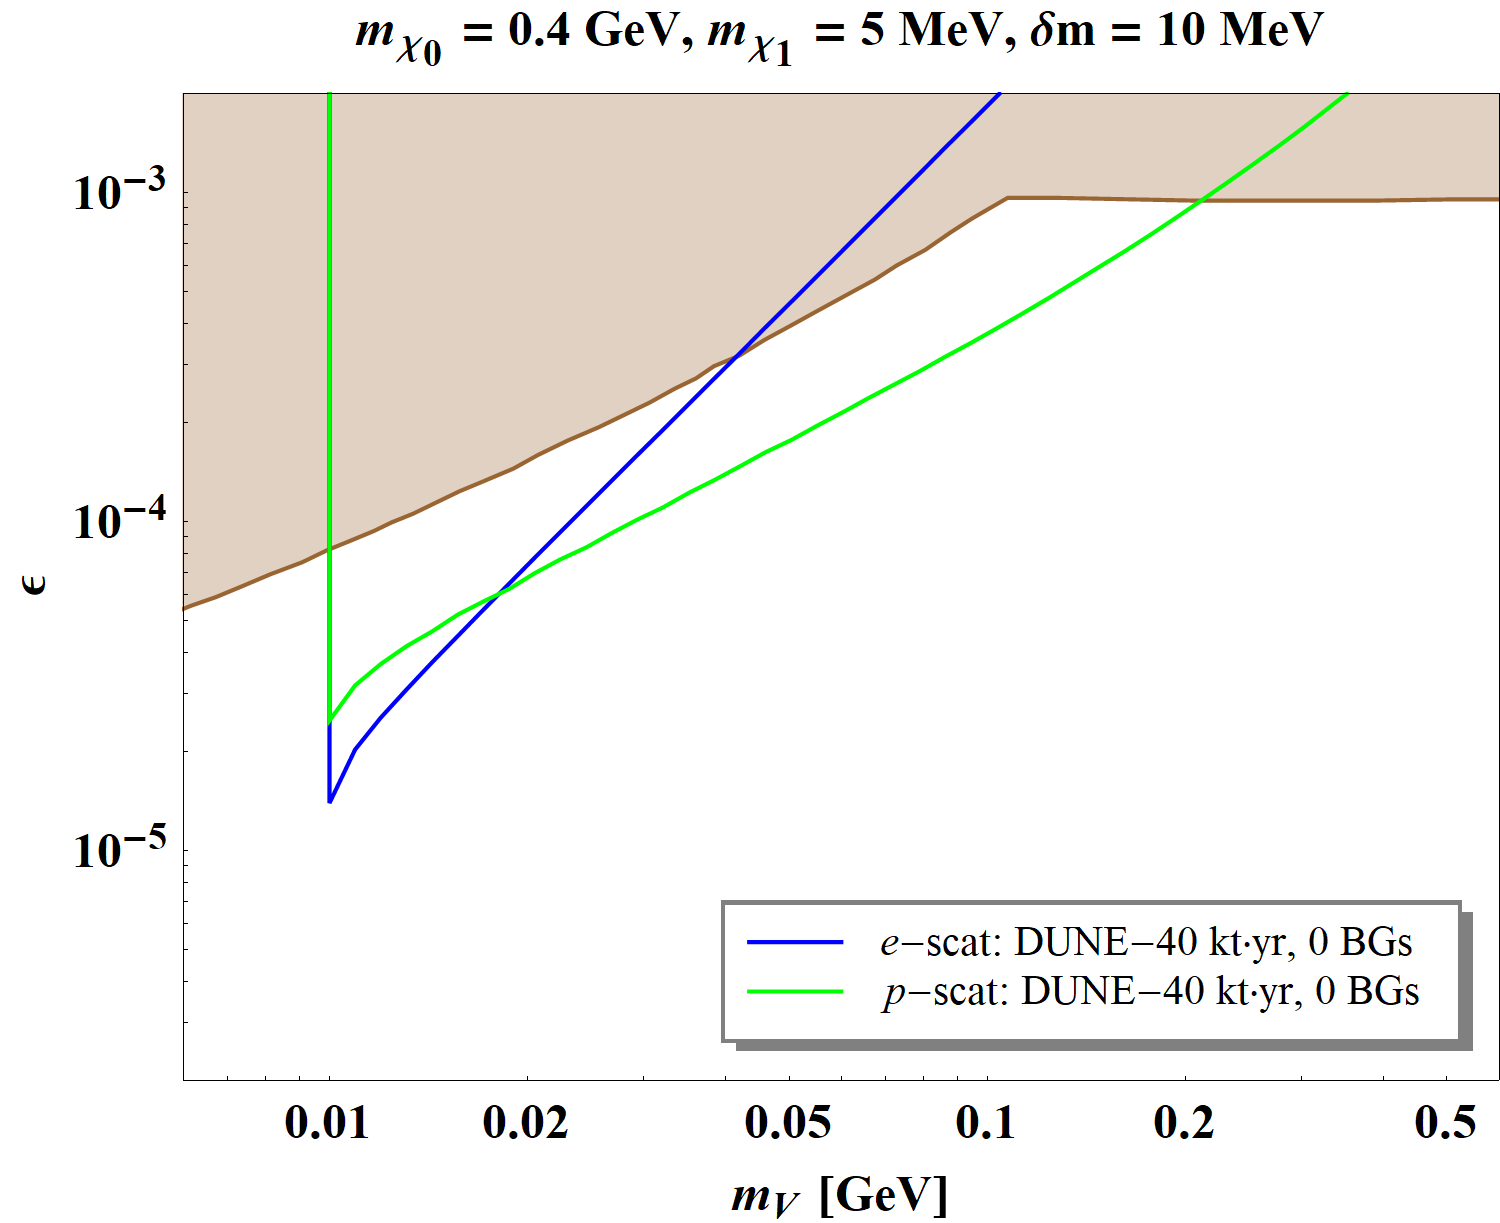
\includegraphics[width=6cm]{inv_PD_vs_DUNE} 
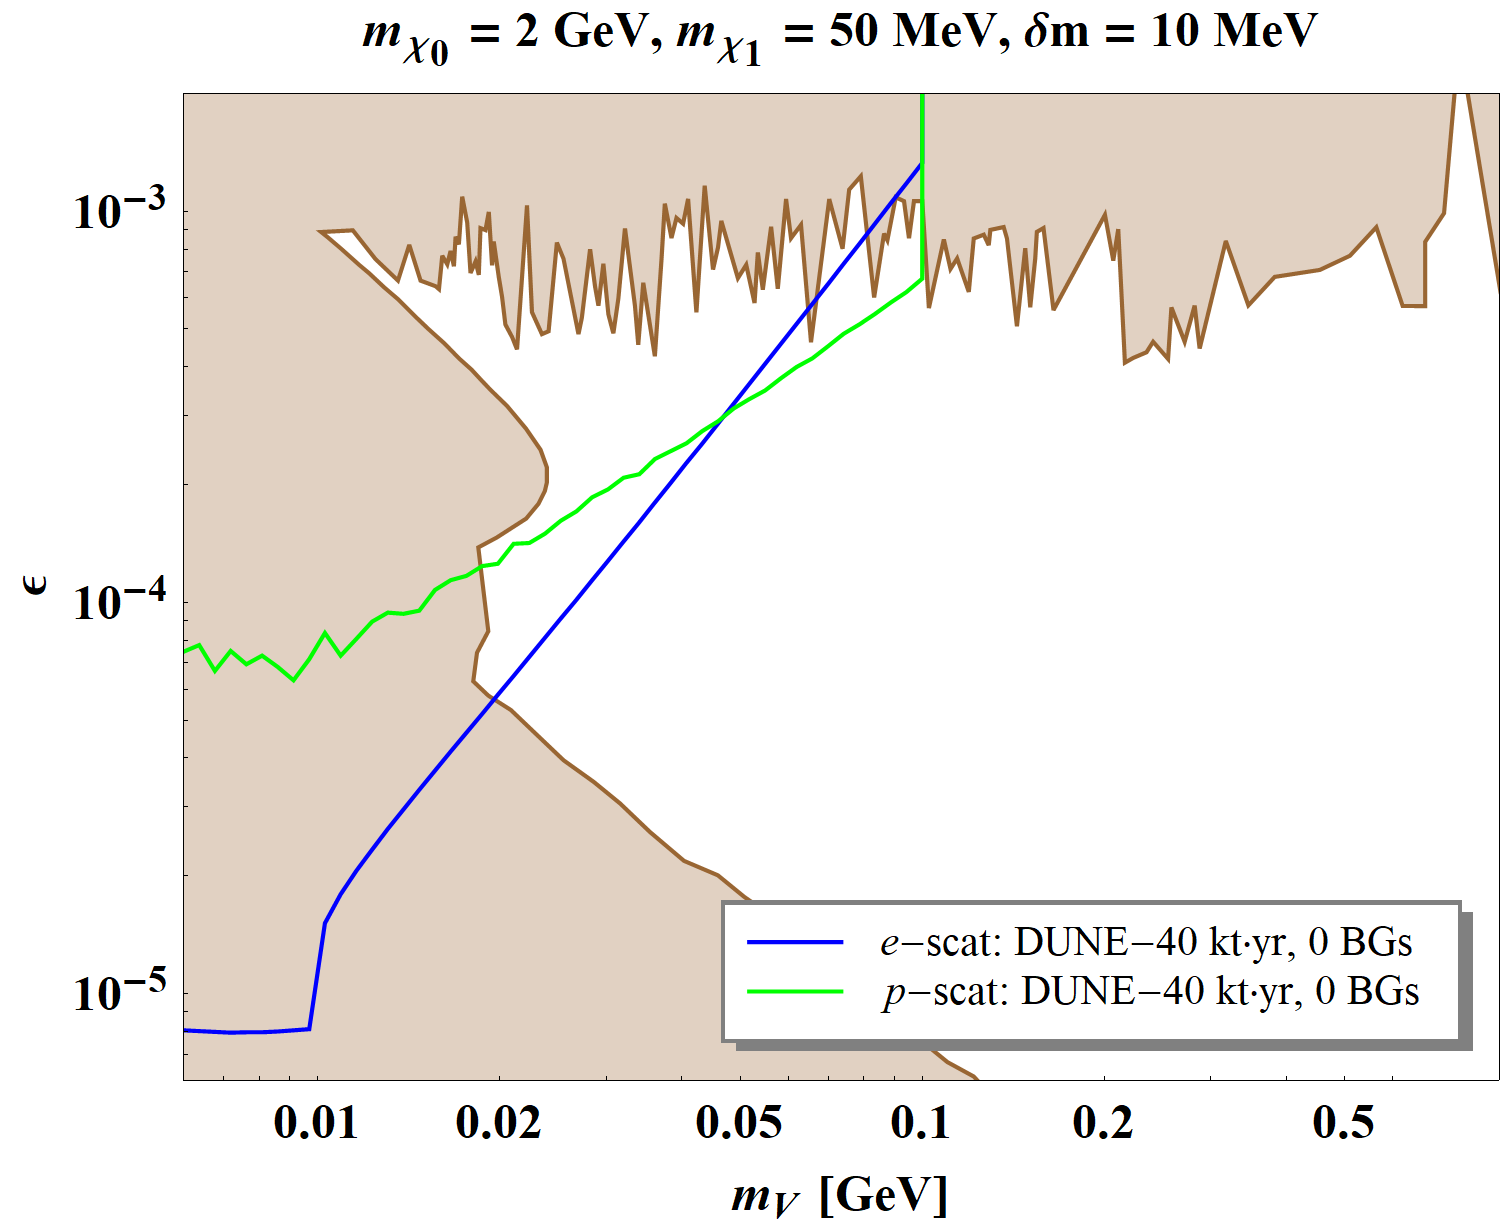
\includegraphics[width=6cm]{vis_PD_vs_DUNE} \\
\vspace{0.3cm}
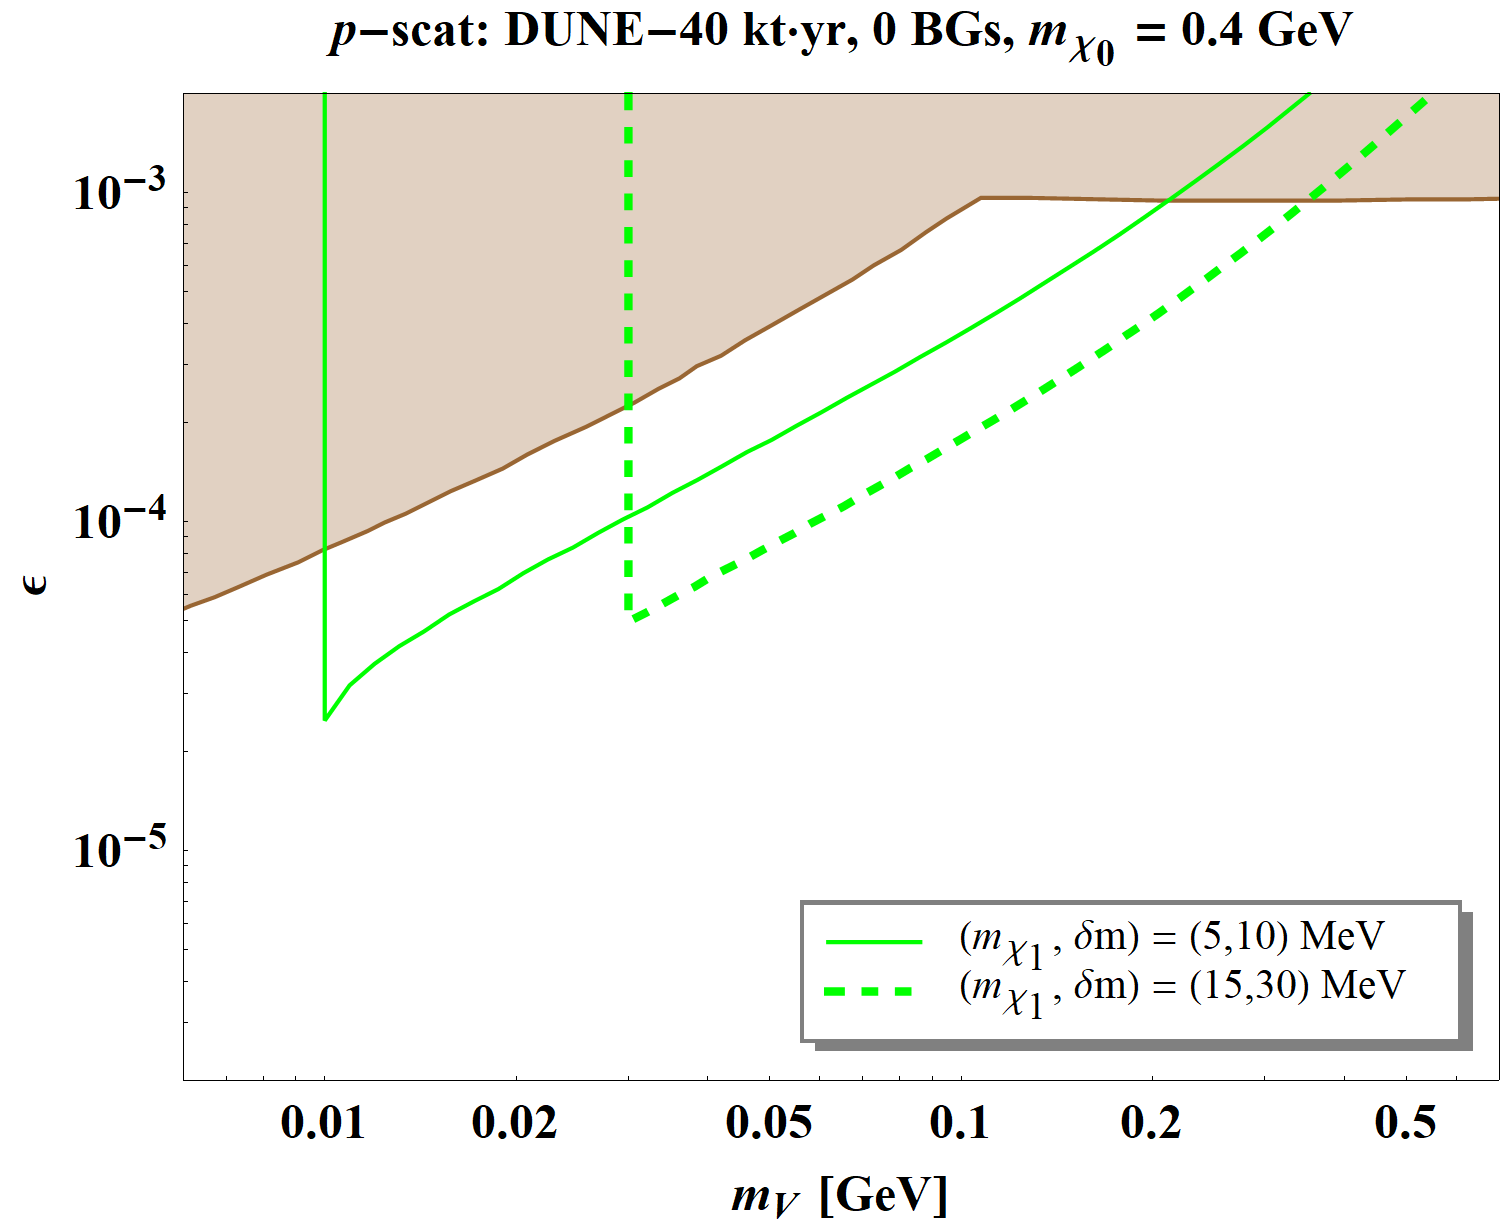
\includegraphics[width=6cm]{inv_DUNE_p-scatterings}
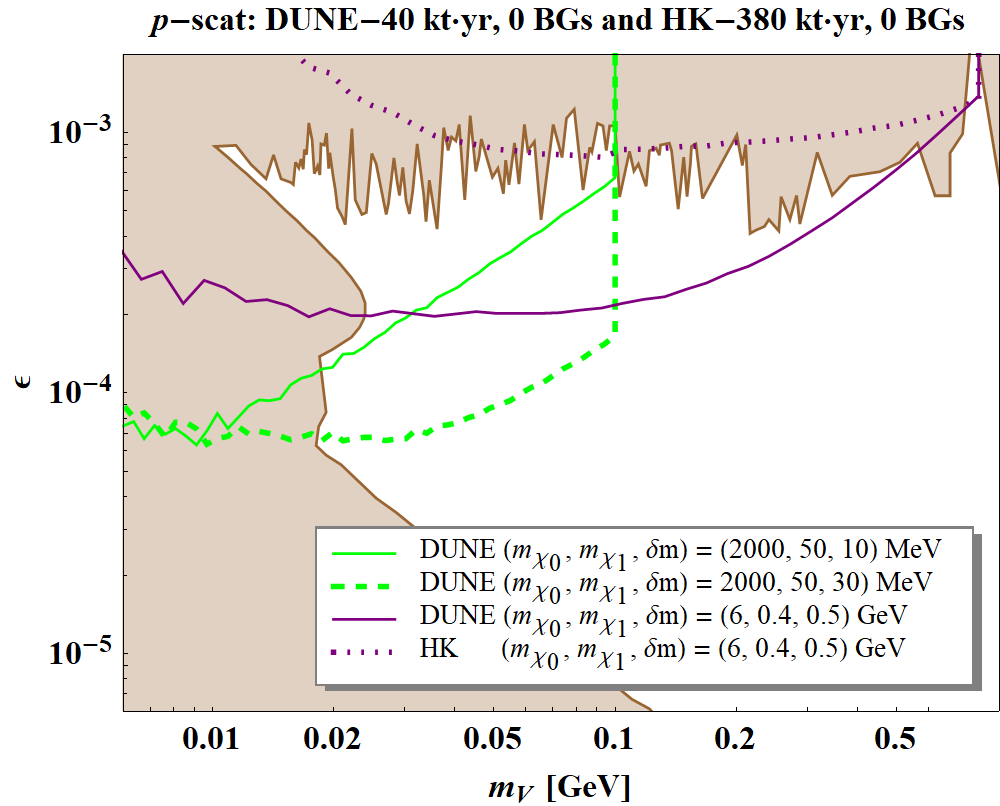
\includegraphics[width=6cm]{vis_DUNE_p-scatterings}
\caption[Experimental sensitivities for $m_{\chi_n}$ values in terms of $m_V - \epsilon$]{
The experimental sensitivities in terms of reference model parameters $m_V - \epsilon$ 
for $m_{\chi_0} = 0.4$ GeV, $m_{\chi_1} = 5$ MeV, and $\delta m = m_{\chi_2} - m_{\chi_1} = 10$ MeV (upper-left panel) and $m_{\chi_0} = 2$ GeV, $m_{\chi_1} = 50$ MeV, and $\delta m = 10$ MeV (upper-right panel).
The left panels are for Scenario 1 and the right ones are for Scenario 2.
The lower panels compare different reference points in the $p$-scattering channel.
See the text for the details.
\label{fig:darkphotonparameter} }
\end{figure}


In displaying the results, we separate the signal categories into %such that
%--
\begin{itemize}
\item Scenario 1: $m_V > 2 m_{\chi_1}$, experimental limits for $V \to$ invisible  applied.
\item Scenario 2: $m_V \le 2 m_{\chi_1}$, experimental limits for $V \to e^+ e^-$ invisible  applied.
\end{itemize}

The brown-shaded region shows the latest limits set by various experiments such as the fixed-target experiment NA64 at the CERN SPS and the B-factory experiment BaBar~\cite{Banerjee:2017hhz}.
The blue solid line describes the experimental sensitivity\footnote{This is defined as the boundary of parameter space that can be probed by the dedicated search in a given experiment at 90\% \dword{cl}, practically obtained from eq.~(\ref{eq:MIsensitivity}).} at DUNE \dword{fd} under a zero background assumption.
The associated exposure is \fdfiducialmass $\cdot$ yr, i.e., a total fiducial volume of 40 kilo-ton times 1-year running time.
For comparison, we also show the sensitivities of DUNE to the $p$-scattering signal as a green solid line. 

Inspired by this potential of searching for the proton scattering channel, we study another reference parameter and compare it with the original one in the lower-left panel of Figure~\ref{fig:darkphotonparameter}. 
We see the reachable $\epsilon$ values rise, as $m_V$ increases. 


For Scenario 2 (the right panels of Figure~\ref{fig:darkphotonparameter}), we choose a different reference parameter set: $m_{\chi_0} = 2$ GeV, $m_{\chi_1} = 50$ MeV, $\delta m = 10$ MeV. 
The current limits (brown shaded regions), from various fixed target experiments, B-factory experiments, and astrophysical observations, are taken from Ref.~\cite{Banerjee:2018vgk}.


We next discuss model-independent experimental sensitivities. 
The experimental sensitivities are determined by the number of signal events excluded at 90\% \dword{cl} in the absence of an observed signal.
The expected number of signal events, $N_{\rm sig}$, is given by
\begin{align}
N_{\rm sig} = \sigma_\epsilon \mathcal F A(\ell_{\rm lab}) t_{\rm exp} N_T\,,
\label{eq:NS}
\end{align}
where $T$ stands for the target that $\chi_1$ scatters off, $\sigma_\epsilon$ is the cross section of the primary scattering $\chi_1 T \to \chi_2 T$, $\mathcal F$ is the flux of $\chi_1$, $t_{\rm exp}$ is the exposure time, and $A(\ell_{\rm lab})$ is the acceptance that is defined as 1 if the event occurs within the fiducial volume and 0 otherwise.
Here we determine the acceptance for an $i$\dword{bdm} signal by the distance between the primary and secondary vertices in the laboratory frame, $\ell_{\rm lab}$, so $A(\ell_{\rm lab}) = 1$ when both the primary and secondary events occur inside the fiducial volume. (Given this definition, obviously, $A(\ell_{\rm lab}) = 1$ for elastic \dword{bdm}.)
%Note that o
Our notation $\sigma_\epsilon$ includes additional realistic effects from cuts, threshold energy, and the detector response, hence it can be understood as the fiducial cross section.

The 90\% \dword{cl} exclusion limit, $N_s^{90}$, can be obtained with a modified frequentist construction~\cite{cls1,cls2}. We follow the methods in Refs.~\cite{Dermisek:2013cxa,Dermisek:2014qca,Dermisek:2016via} in which the Poisson likelihood is assumed. 
An experiment becomes sensitive to the signal model independently if $N_{\rm sig} \ge N_s^{90}$.
Plugging eq.~\eqref{eq:NS} here, we find the experimental sensitivity expressed by %the following inequality
\begin{align}
\sigma_\epsilon \mathcal F \ge \frac{N_s^{90}}{A(\ell_{\rm lab}) t_{\rm exp} N_T}\,. 
\label{eq:MIsensitivity}
\end{align}
Since $\ell_{\rm lab}$ differs event-by-event, we take the maximally possible value of laboratory-frame mean decay length, i.e., $\bar{\ell}_{\rm lab}^{\rm max} \equiv \gamma_{\chi_2}^{\max} \bar{\ell}_{\rm rest}$ where $\gamma_{\chi_2}^{\max}$ is the maximum boost factor of $\chi_2$ and $\bar{\ell}_{\rm rest}$ is the rest-frame mean decay length. 
We emphasize that this is a rather conservative approach, because the acceptance $A$ is inversely proportional to $\ell_{\rm lab}$.
We then show the experimental sensitivity of any kind of experiment for a given background expectation, exposure time, and number of targets, in the plane of $\bar{\ell}_{\rm lab}^{\rm max} - \sigma_\epsilon \cdot \mathcal F$. 
The left panel of Figure~\ref{fig:modelindependent} demonstrates the expected model-independent sensitivities at the DUNE experiment.
%several experiments. 
%The red (orange) line is for the \dword{protodune} detectors with the assumptions of 100 (zero) background events and 470 t$\cdot$yr exposure, while 
The green (blue) line is for the DUNE \dword{fd} with a background-free assumption and 20 (40) kt$\cdot$yr exposure.

\begin{figure}[t]
\centering
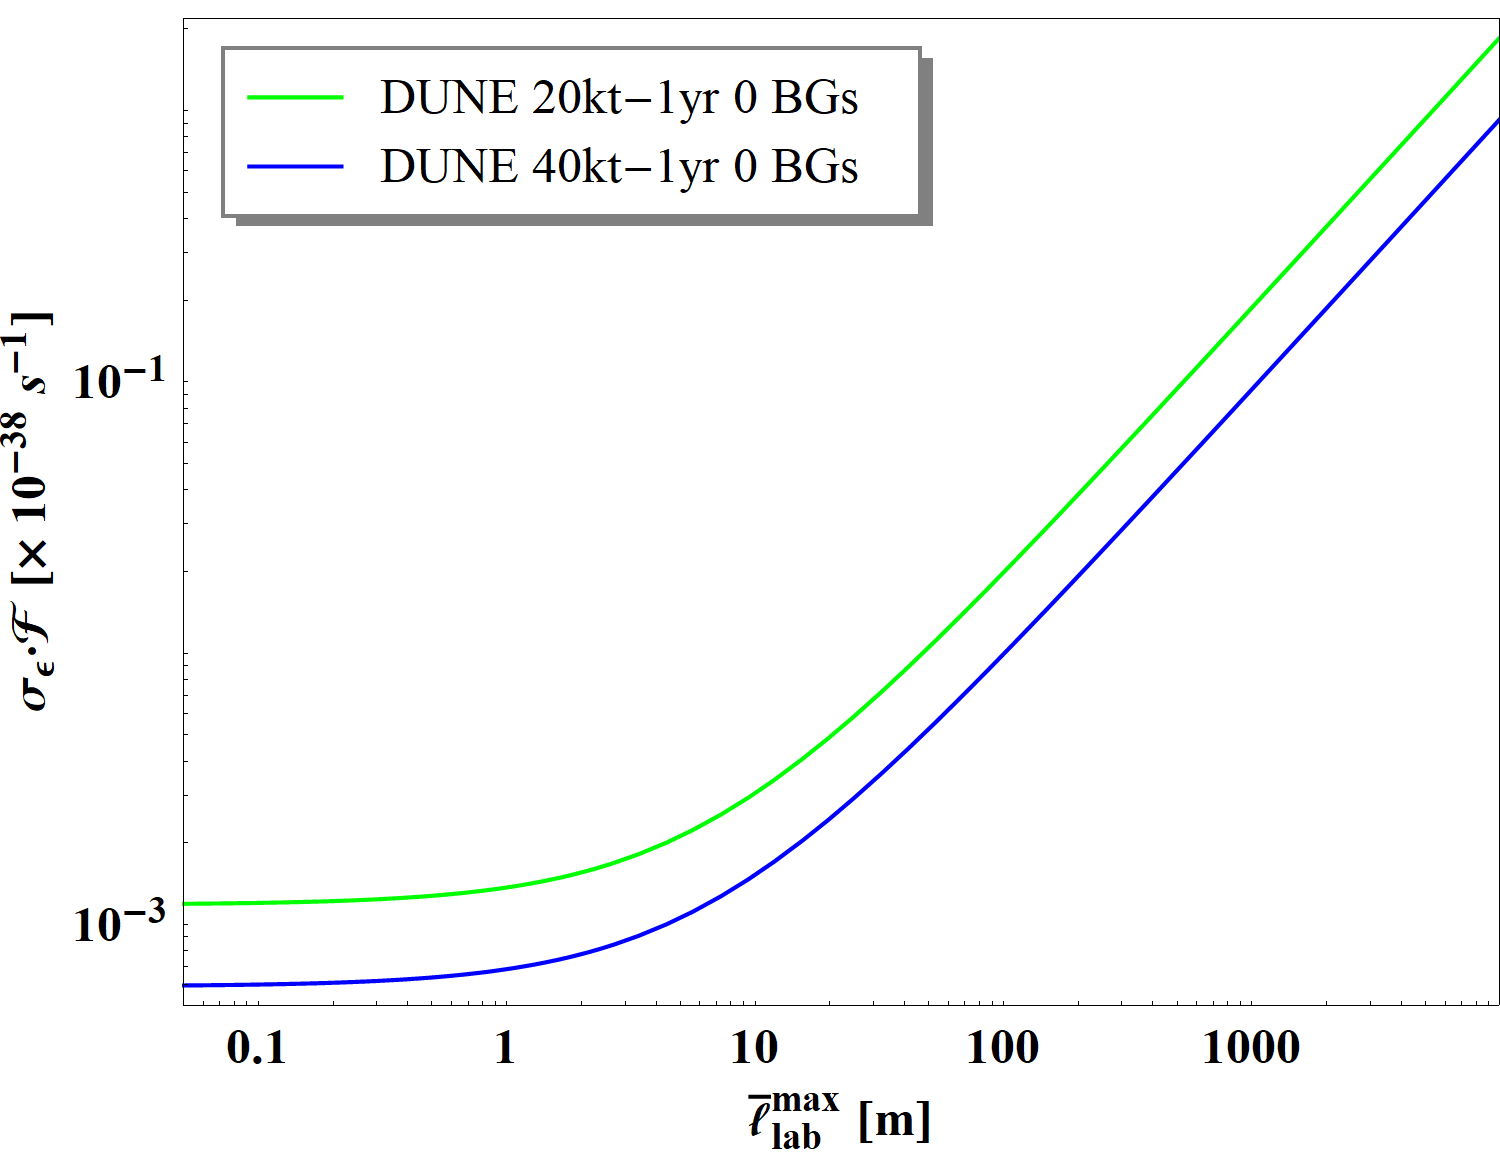
\includegraphics[width=6cm]{SigmaFluxVslMaxLab_TotalOnly}
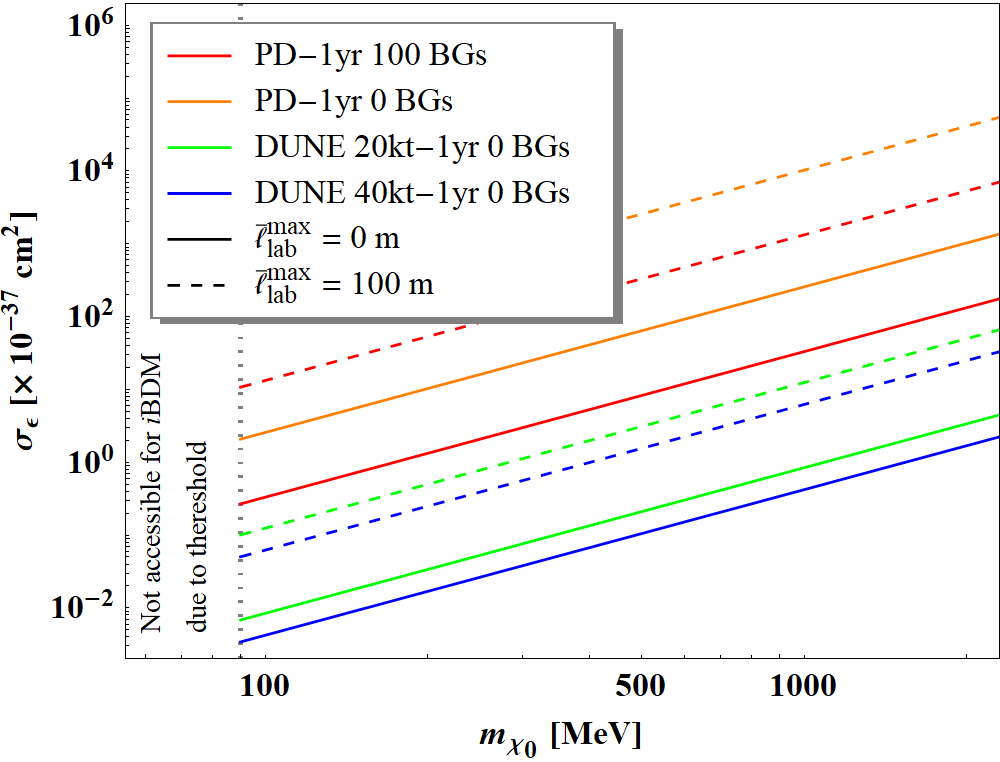
\includegraphics[width=6cm]{SigmaVsE1}
\caption[Model-independent experimental sensitivities of $i$BDM search]{
Left: model-independent experimental sensitivities of $i$\dword{bdm} search in $\bar{\ell}_{\rm lab}^{\rm max} - \sigma_\epsilon \cdot \mathcal F$ plane. 
The reference experiments are
%\dword{protodune} with 100 background (red), zero-background (orange) assumption for 1-year time exposure, 
DUNE 20kt (green), and DUNE 40kt (blue) with zero-background assumption for 1-year time exposure. 
Right: Experimental sensitivities of $i$\dword{bdm} search in $m_{\chi_0} - \sigma_\epsilon$ plane. The sensitivities for $\bar{\ell}_{\rm lab}^{\rm max} = 0$ m and 100 m are shown as solid and dashed lines for each reference experiment in the left panel.
\label{fig:modelindependent} }
\end{figure}

The right panel of Figure~\ref{fig:modelindependent} reports model-dependent sensitivities for $\bar{\ell}_{\rm lab}^{\rm max} = 0$ m and 100 m corresponding to the experiments in the left panel.
Note that this %way 
method of presentation is reminiscent of the widely known scheme for showing the experimental reaches in various \dword{dm} direct detection experiments, i.e., $m_{\rm DM} - \sigma_{\rm DM - target}$ where $m_{\rm DM}$ is the mass of \dword{dm} and $\sigma_{\rm DM - target}$ is the cross section between the \dword{dm} and target. 
For the case of non-relativistic \dword{dm} scattering in the direct-detection experiments, $m_{\rm DM}$ determines the kinetic energy scale of the incoming \dword{dm}, just like $m_{\chi_0}$ sets out the incoming energy of boosted $\chi_1$ in the $i$\dword{bdm} search. 

%%%%%%%%%%%%%%%%%%%%%%%%%
\subsection{Elastic Boosted Dark Matter from the Sun \label{sec:FDsun}}

%%%%%%%%%%%%%%%%%%%%%%%%%
\subsubsection{\label{sec:level2} Introduction and theoretical framework}


In this section, we focus on the Benchmark Model ii) discussed in Section~\ref{sec:model}. This study represents the first assessment of sensitivity to this model in DUNE using DUNE's full event generation and detector simulation. We focus on \dword{bdm} flux sourced by \dword{dm} annihilation in the core of the sun. \dword{dm} particles can be captured through their scattering with the nuclei within the sun, mostly hydrogen and helium. This makes the core of the sun a region with concentrated \dword{dm} distribution. The \dword{bdm} flux is
\begin{eqnarray} \label{eq:fluxbdm}
\Phi= f \frac{A}{4\pi D^2},
\end{eqnarray}
where $A$ is the annihilation rate, and $D = 1\,\rm{\dword{au}}$ is the distance from the sun. $f$ is a model-dependent parameter, where $f = 2$ for two-component \dword{dm} as considered here.

For the parameter space of interest, %we are interested in, 
assuming that the 
\dword{dm} annihilation cross section is not too small, the \dword{dm} distribution in the sun has reached an equilibrium between capture and annihilation. This helps to eliminate the annihilation cross section dependence in our study. The chain of processes involved in giving rise to the boosted DM signal from the Sun is illustrated in Fig.~\ref{fig:processes}.
\begin{figure}[h!]
  \centering
  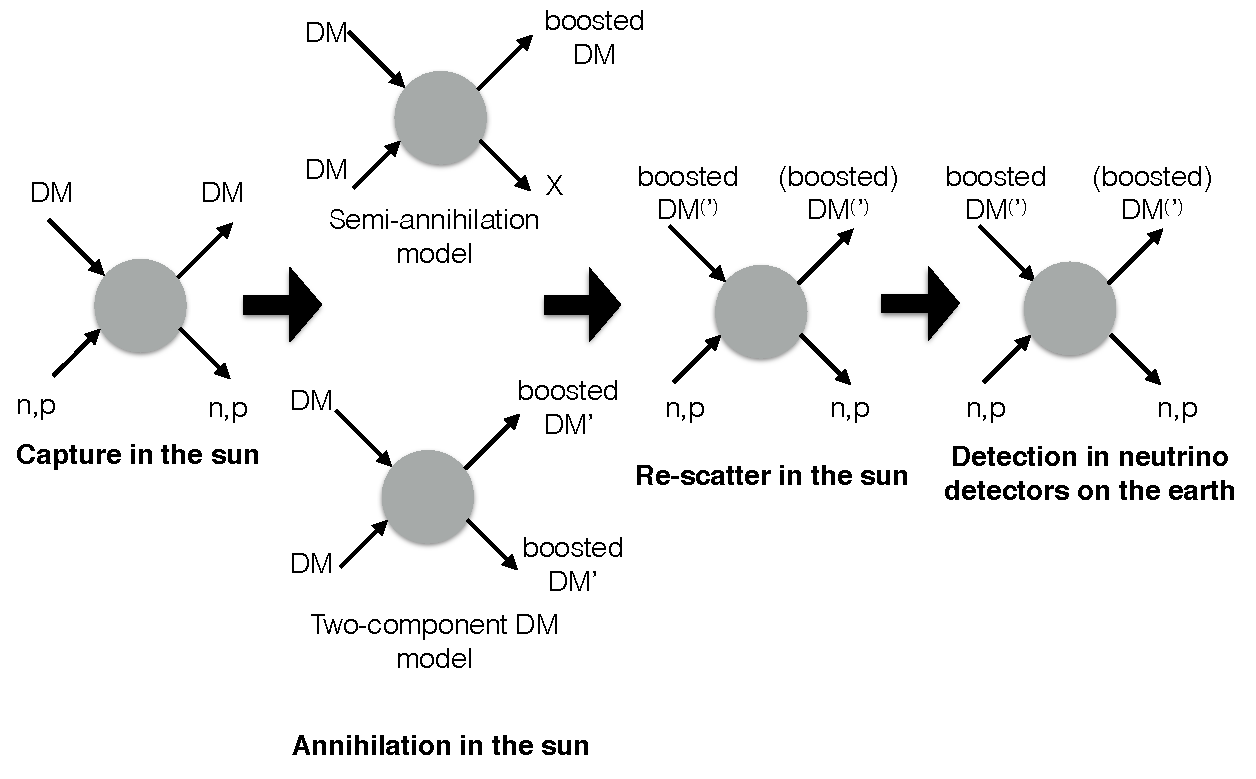
\includegraphics[width=0.7\textwidth]{processes.pdf}
  \caption[Processes leading to boosted DM signal from the sun]{The chain of processes leading to boosted DM signal from the sun. The semi-annihilation and two-component DM models refer to the two examples of the non-minimal dark-sector scenarios introduced in the beginning of Section~\ref{sec:DM}. DM' denotes the lighter DM in the two-component DM model. $X$ is a lighter dark sector particle that may decay away.}
    \label{fig:processes}
\end{figure}

Two additional comments are in order. First, the \dword{dm} particles cannot be too light, i.e.,  lighter than 4\,GeV~\cite{Griest:1986yu,Gould:1987ju}, otherwise we will lose most of the captured \dword{dm} through evaporation rather than annihilation; this would dramatically reduce the \dword{bdm} flux. Additionally, one needs to check that \dword{bdm} particles cannot lose energy and potentially be recaptured by scattering with the solar material when they escape from the core region after production. Rescattering is found to be rare for the benchmark models considered in this study and we consider the \dword{bdm} flux to be monochromatic at its production energy.

The event rate to be observed at DUNE is 
\begin{equation}
R = \Phi \times \sigma_{\rm{SM} - \chi} \times \varepsilon \times N,
\end{equation}
 where $\Phi$ is the flux given by Eq. \eqref{eq:fluxbdm}, $\sigma_{\rm{SM} - \chi}$ is the scattering cross section of the \dword{bdm} off of \dword{sm} particles, $\varepsilon$ is the efficiency of the detection of such a process, and $N$ is the number of target particles in DUNE. The computation of the flux of \dword{bdm} from the sun can be found in~\cite{Berger:2014sqa}. 

The processes of typical BDM scattering in argon are illustrated in Fig.~\ref{fig:BDM-argon}.
We generate the signal events and calculate interaction cross sections in the detector using a newly developed \dword{bdm} module~\cite{Andreopoulos:2009rq,Andreopoulos:2015wxa,Berger:2018} that includes elastic and deep inelastic scattering, as well as a range of nuclear effects. This conservative event generation neglects the dominant contributions from baryon resonances in the final state hadronic invariant mass range of 1.2 to 1.8 GeV, which should not have a major effect on our main results. The interactions are taken to be mediated by an axial, flavor-universal $Z^\prime$ coupling to both the \dword{bdm} and with the quarks. The axial charge is taken to be 1. 
% The resulting cross-sections with argon are shown in Tab.~\ref{tab:eff-tab}. 
The events are generated for the \nominalmodsize DUNE detector module~\cite{dunetpc_code}, though we only study the dominant scattering off of the \argon40 atoms therein. The method for determining the efficiency $\varepsilon$ is described below. The number of target argon atoms is $N = 1.5  \times 10^{32}$ assuming a target mass of \nominalmodsize{}.

\begin{figure}[h!]
  \centering
  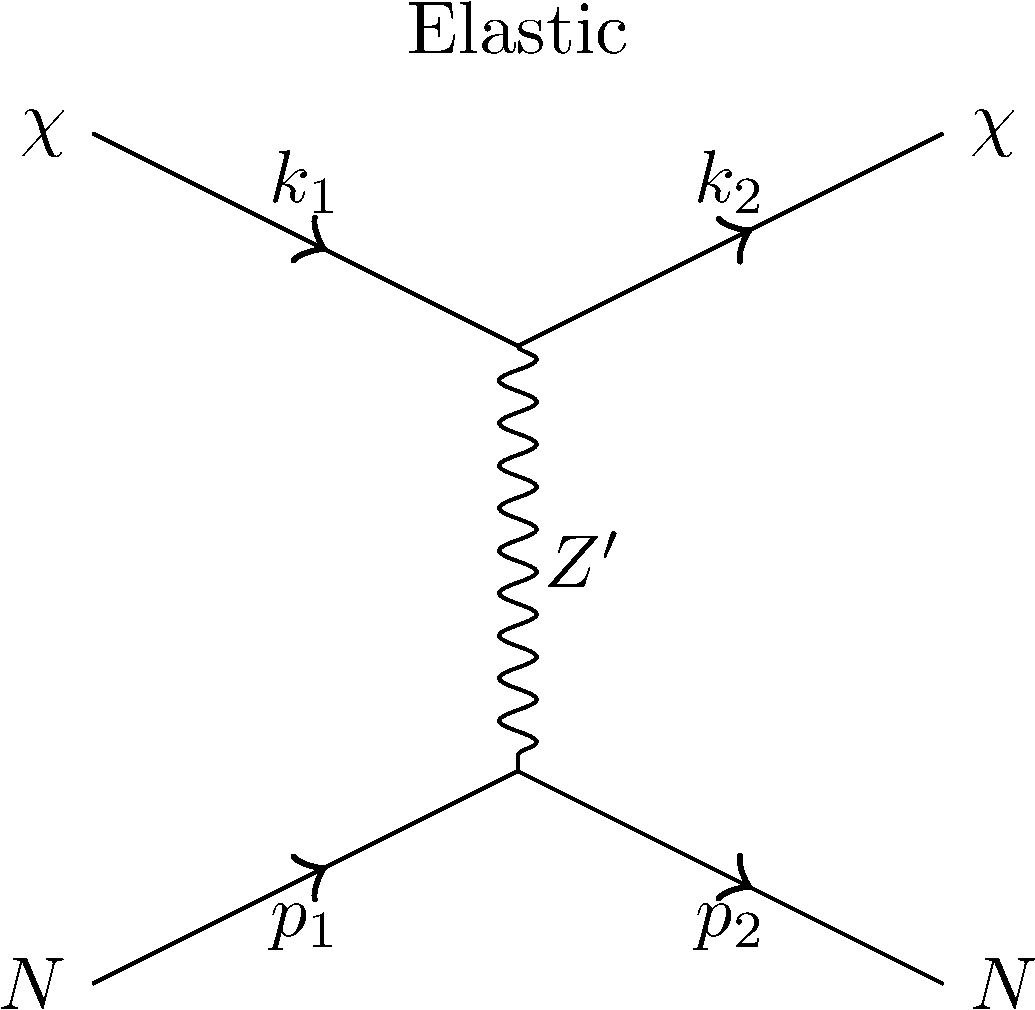
\includegraphics[width=0.256\textwidth]{elastic-diagram.pdf}
  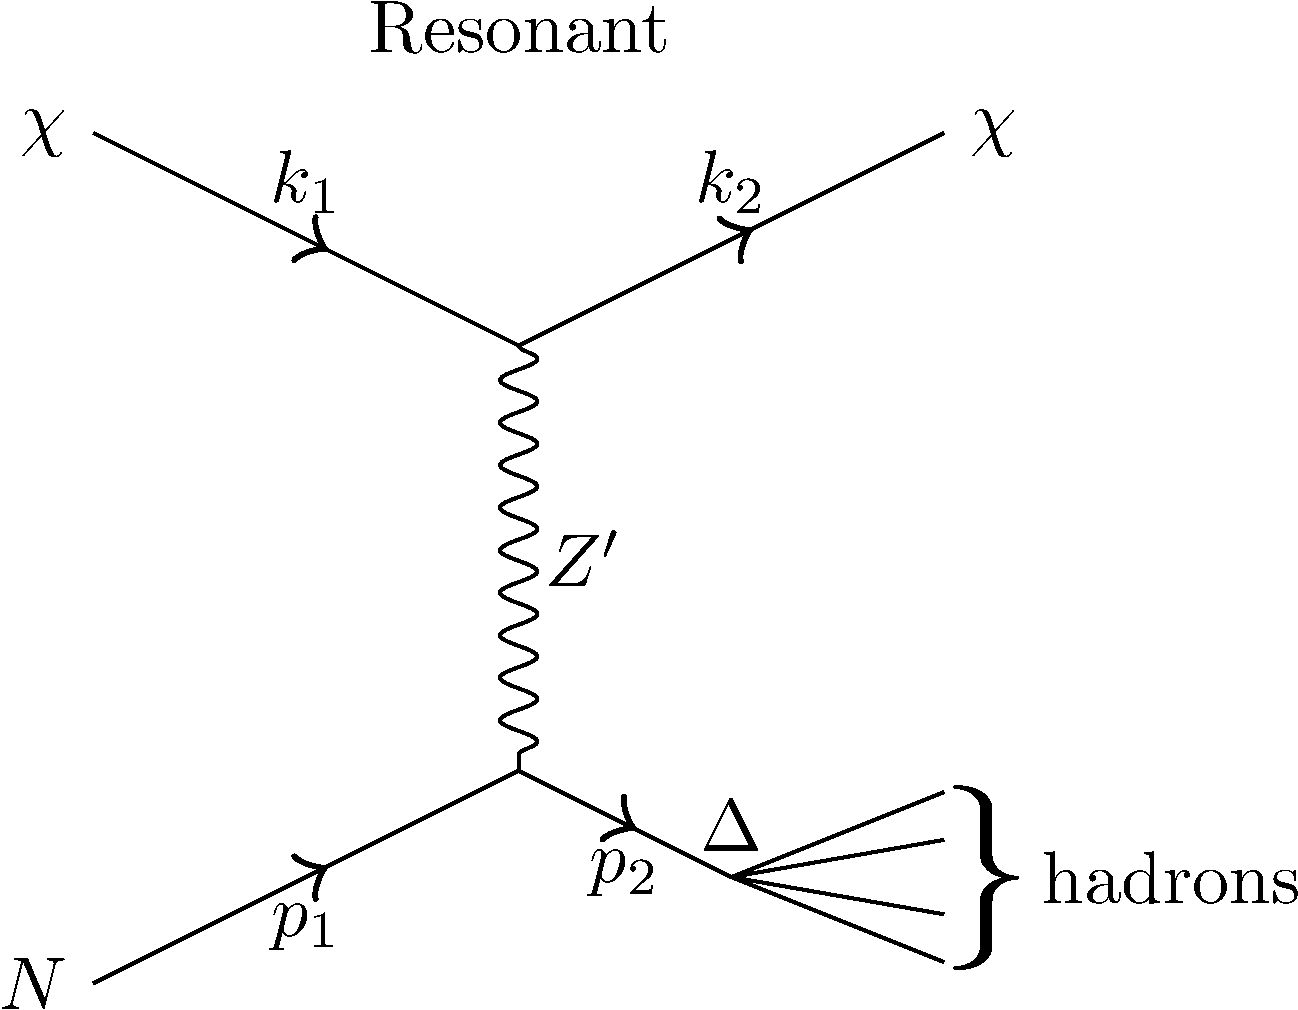
\includegraphics[width=0.33\textwidth]{resonant-diagram.pdf}
  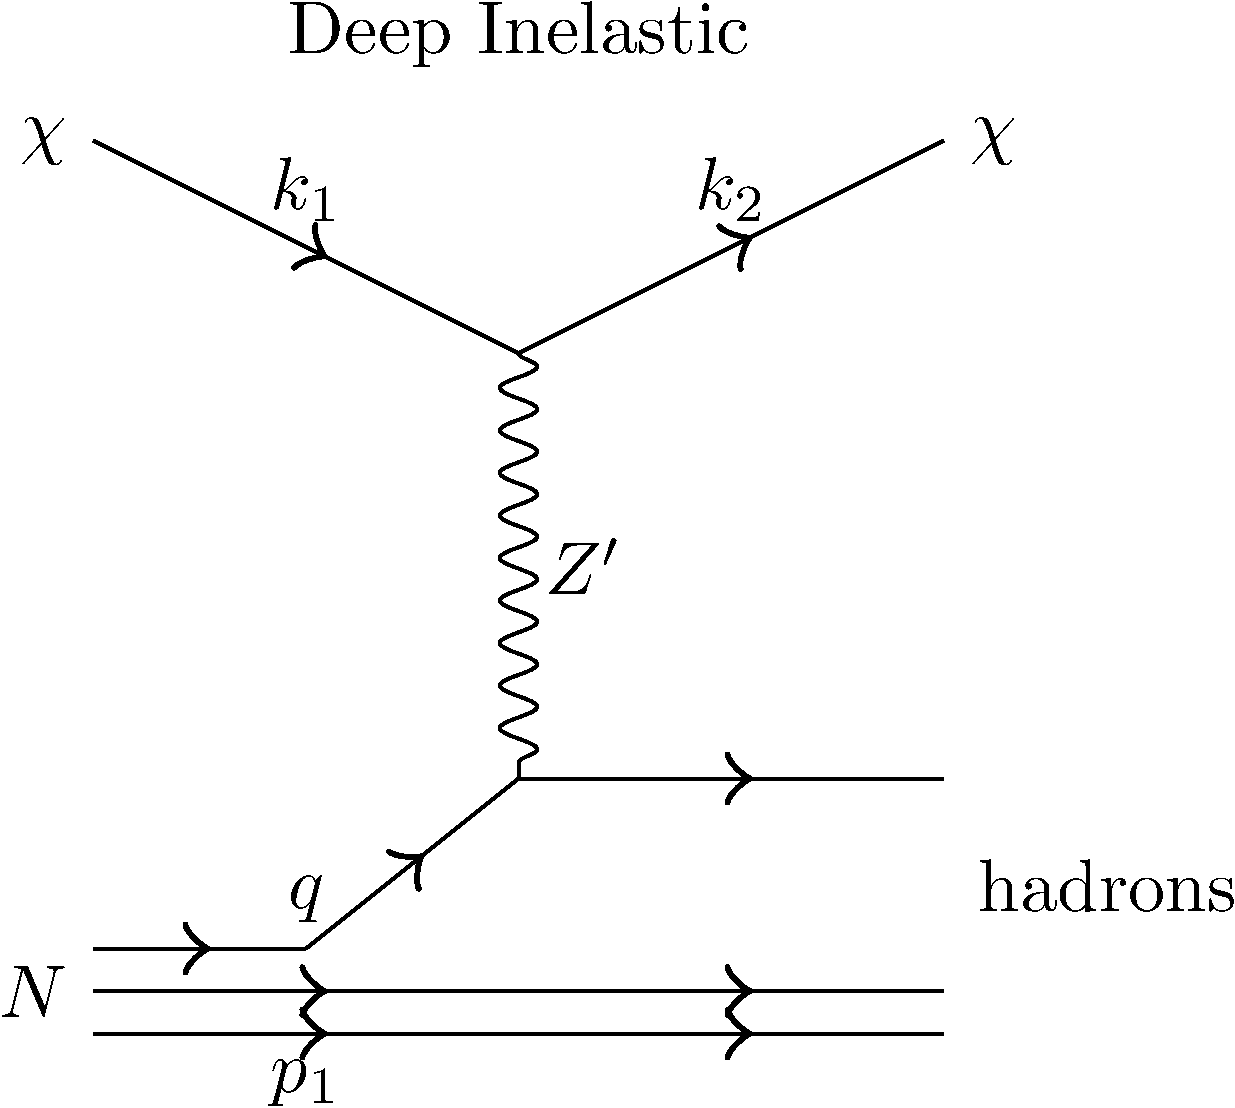
\includegraphics[width=0.29\textwidth]{deepinelastic-diagram.pdf}
  \caption{Diagram illustrating each of the three processes contributing to dark matter scattering in argon: elastic (left), baryon resonance (middle), and deep inelastic (right).}
  \label{fig:BDM-argon}
\end{figure}
% -------------------------------------------------------------------------------
\subsubsection{Background Estimation}
\label{sec:background}

The main background in this process comes from the \dword{nc} 
interactions of atmospheric neutrinos and argon,
as they share the features that the timing of events is unknown in advance,
and that the interactions with argon produce hadronic activity in the detector.
We use \dword{genie}~\cite{Andreopoulos:2009rq,Andreopoulos:2015wxa}
interfaced by the \dword{larsoft} toolkit to generate the \dword{nc} atmospheric
neutrino events, and obtain 845 events in a \nominalmodsize{} module for one year of
exposure.

%%%%%%%%%%%%%%%%%%%%%%%%%
\subsubsection{Detector Response}
\label{sec:detector_resp}

The finite detector resolution is taken into
account by smearing the direction of the stable final state particles, 
including protons, neutrons, charged pions, muons, electrons, and photons,
with the expected angular resolution,
and by ignoring the ones with kinetic energy below detector threshold,
using the parameters reported in the DUNE \dword{cdr}~\cite{Acciarri:2015uup}.
We form as the observable the total momentum from all the stable final state particles,
and obtain its angle with respect to the direction of the sun.
The sun position is simulated with the SolTrack package~\cite{SolTrack}
including the geographical coordinates of the DUNE \dword{fd}~\cite{DUNE_DocDB136}.
We consider both the scenarios in which we can reconstruct neutrons and in which 
neutrons will not be reconstructed.
Figure~\ref{fig:m10_SmearedReconstructableAngle} shows the angular distributions of
the \dword{bdm} signals with mass of 10\,GeV and different boost factors,
and of the background events.

% ---------------------------------------------------------------------------------
\begin{figure*}[!htb]
\centering
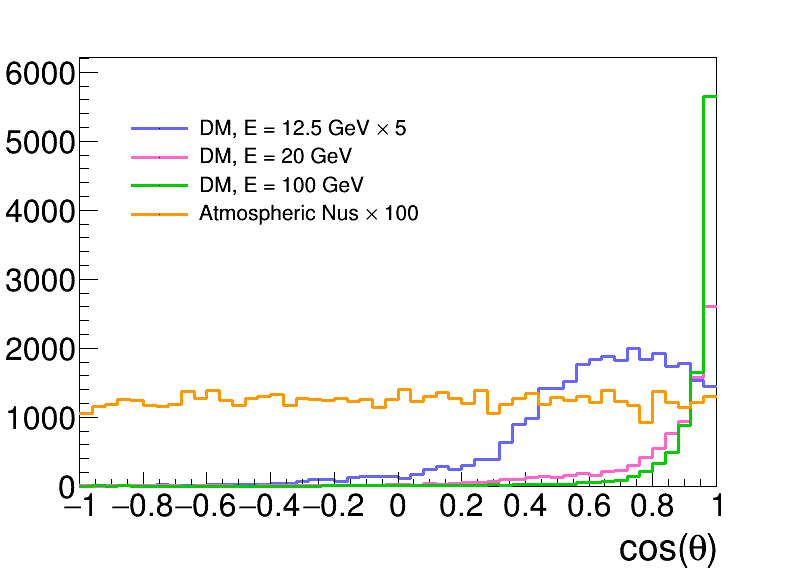
\includegraphics[width=0.45\textwidth]{m10_SmearedReconstructableAngle.png}
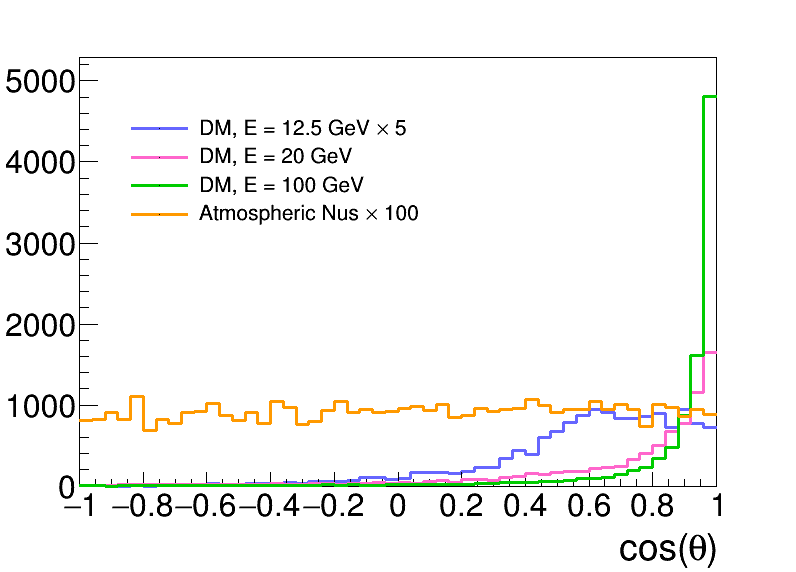
\includegraphics[width=0.45\textwidth]{m10_SmearedReconstructableNoNAngle.png}
\caption[Angular distribution of the BDM signal events for a BDM mass of 10\,GeV]{Angular distribution of the \dword{bdm} signal events for a \dword{bdm} mass of 10\,GeV
and different boosted factors, $\gamma$, and of the atmospheric neutrino NC
background events.
$\theta$ represents the angle of the sum over all the stable final state
particles as detailed in the text.
The amount of background represents one-year data collection, magnified by a factor 100,
while the amount of signal reflects the detection efficiency of 10,000 \dword{mc} events, as
described in this note.
The left plot shows the scenario where neutrons can be reconstructed,
while the right plot represents the scenario without neutrons.}
\label{fig:m10_SmearedReconstructableAngle}
\end{figure*}
% ---------------------------------------------------------------------------------


To increase the signal fraction in our samples, we select events with $\cos\theta > 0.6$,
and obtain the selection efficiency $\varepsilon$ for different \dword{bdm} models.
% as listed in Table~\ref{tab:eff-tab}, 
We predict that $104.0 \pm 0.7$ and $79.4 \pm 0.6$ background events per year, in the scenarios with and without neutrons respectively, survive the selection in a DUNE \nominalmodsize module.

%%%%%%%%%%%%%%%%%%%%%%%%%
\subsubsection{Results}

\begin{figure*}[!htb]
\centering
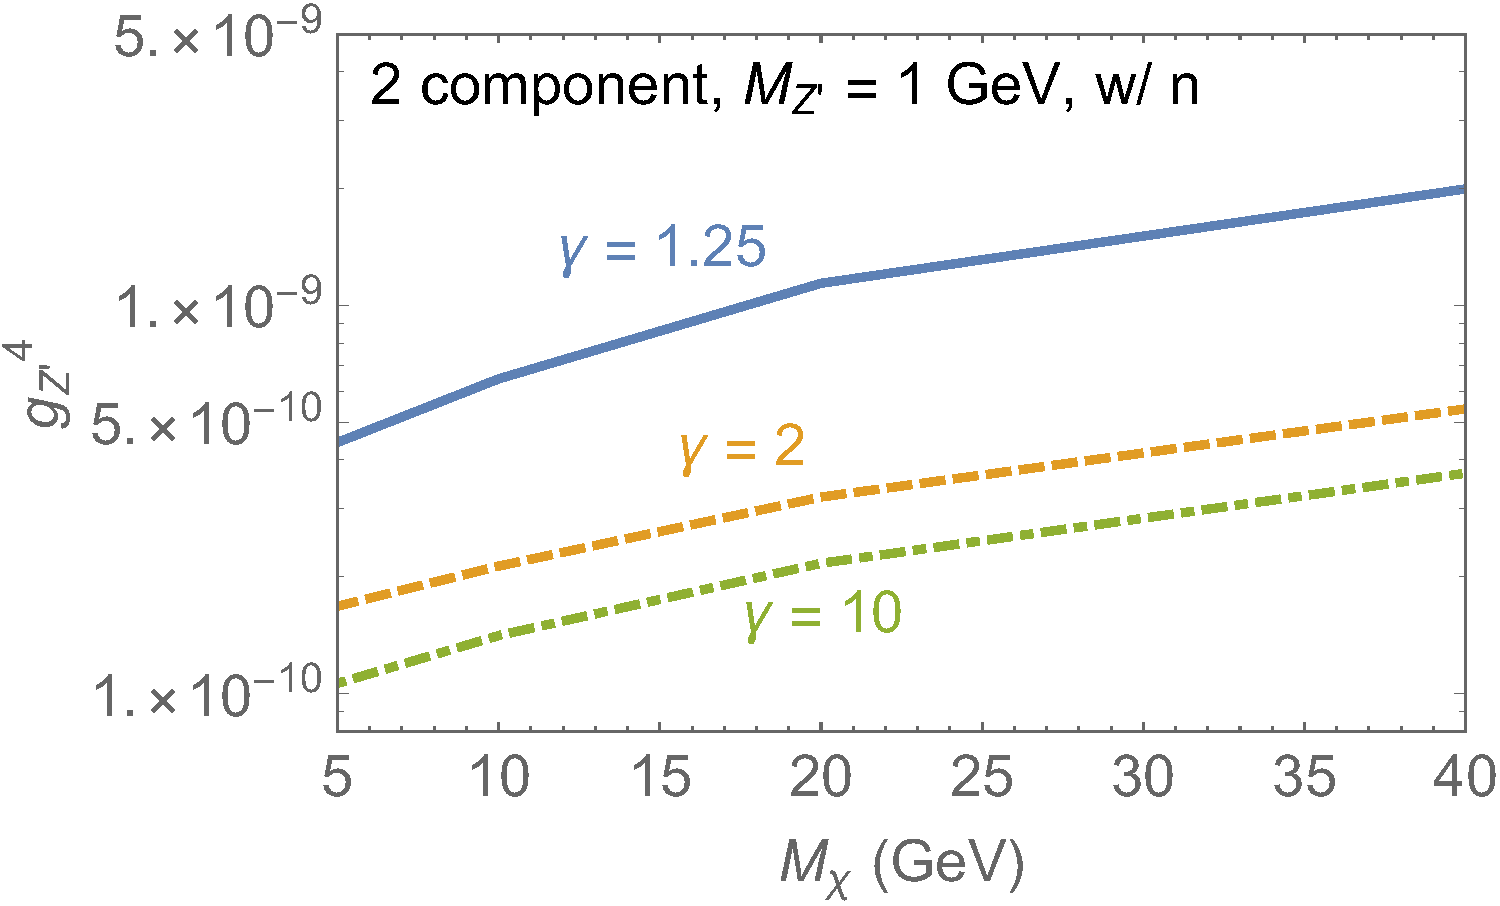
\includegraphics[width=0.45\textwidth]{expected-discovery-with-n.pdf}\hspace{0.05\textwidth}
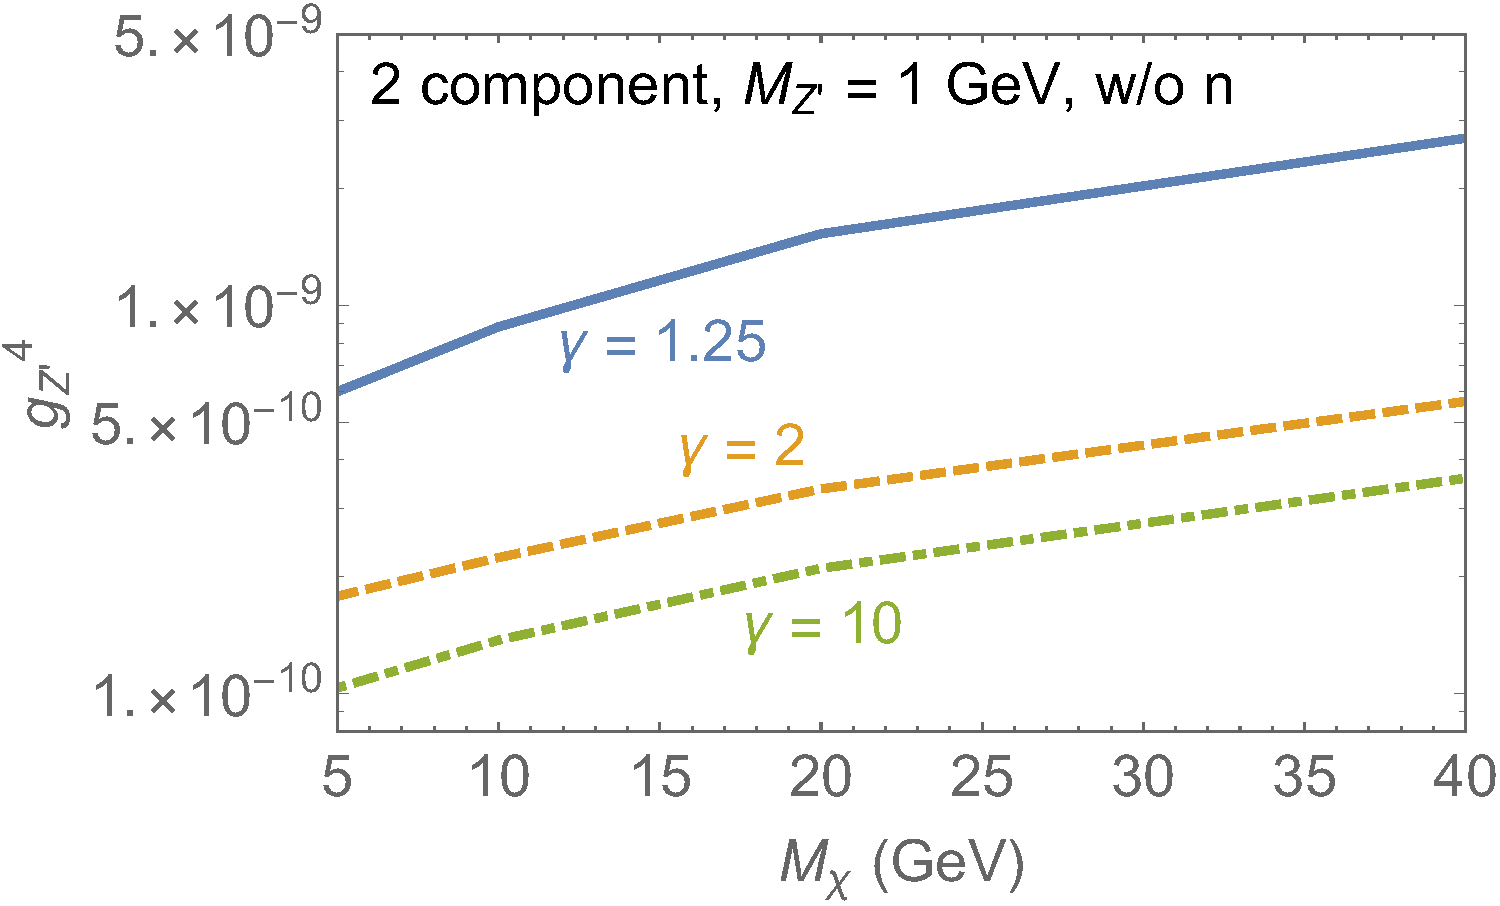
\includegraphics[width=0.45\textwidth]{expected-discovery-no-n.pdf}
\caption[Expected $5\sigma$ discovery reach with one year of DUNE livetime]{Expected $5\sigma$ discovery reach with one year of DUNE livetime for one \nominalmodsize module including neutrons in reconstruction (left) and excluding neutrons (right).\label{fig:significance}}
\end{figure*}
The resulting expected sensitivity is presented in Figure~\ref{fig:significance} in terms of the \dword{dm} mass and the $Z^\prime$ gauge coupling for potential \dword{dm} boosts of $\gamma = 1.25,2,10$ and for a fixed mediator mass of $m_{Z^\prime} = 1~{\rm GeV}$.  We assume a DUNE livetime of one year for one \nominalmodsize module.  The models presented here are currently unconstrained by direct detection searches if the thermal relic abundance of the \dword{dm} is chosen to fit current observations.
Figure~\ref{fig:bdm_sensitivity_comparison} compares the sensitivity of 10 years of data collected in DUNE (40~kton) to re-analyses of the results from other experiments, including Super Kamiokande~\cite{Fechner:2009aa} and \dword{dm} direct detection, PICO-60~\cite{Amole:2019fdf} and PandaX~\cite{Xia:2018qgs}. 

% -----------------------------------------------------------------------
\begin{figure*}[!htb]
\centering
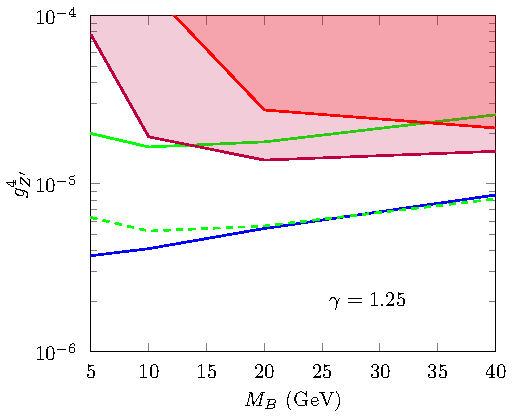
\includegraphics[width=0.45\textwidth]{bdm_preliminary_125_sa}\hspace{0.05\textwidth}
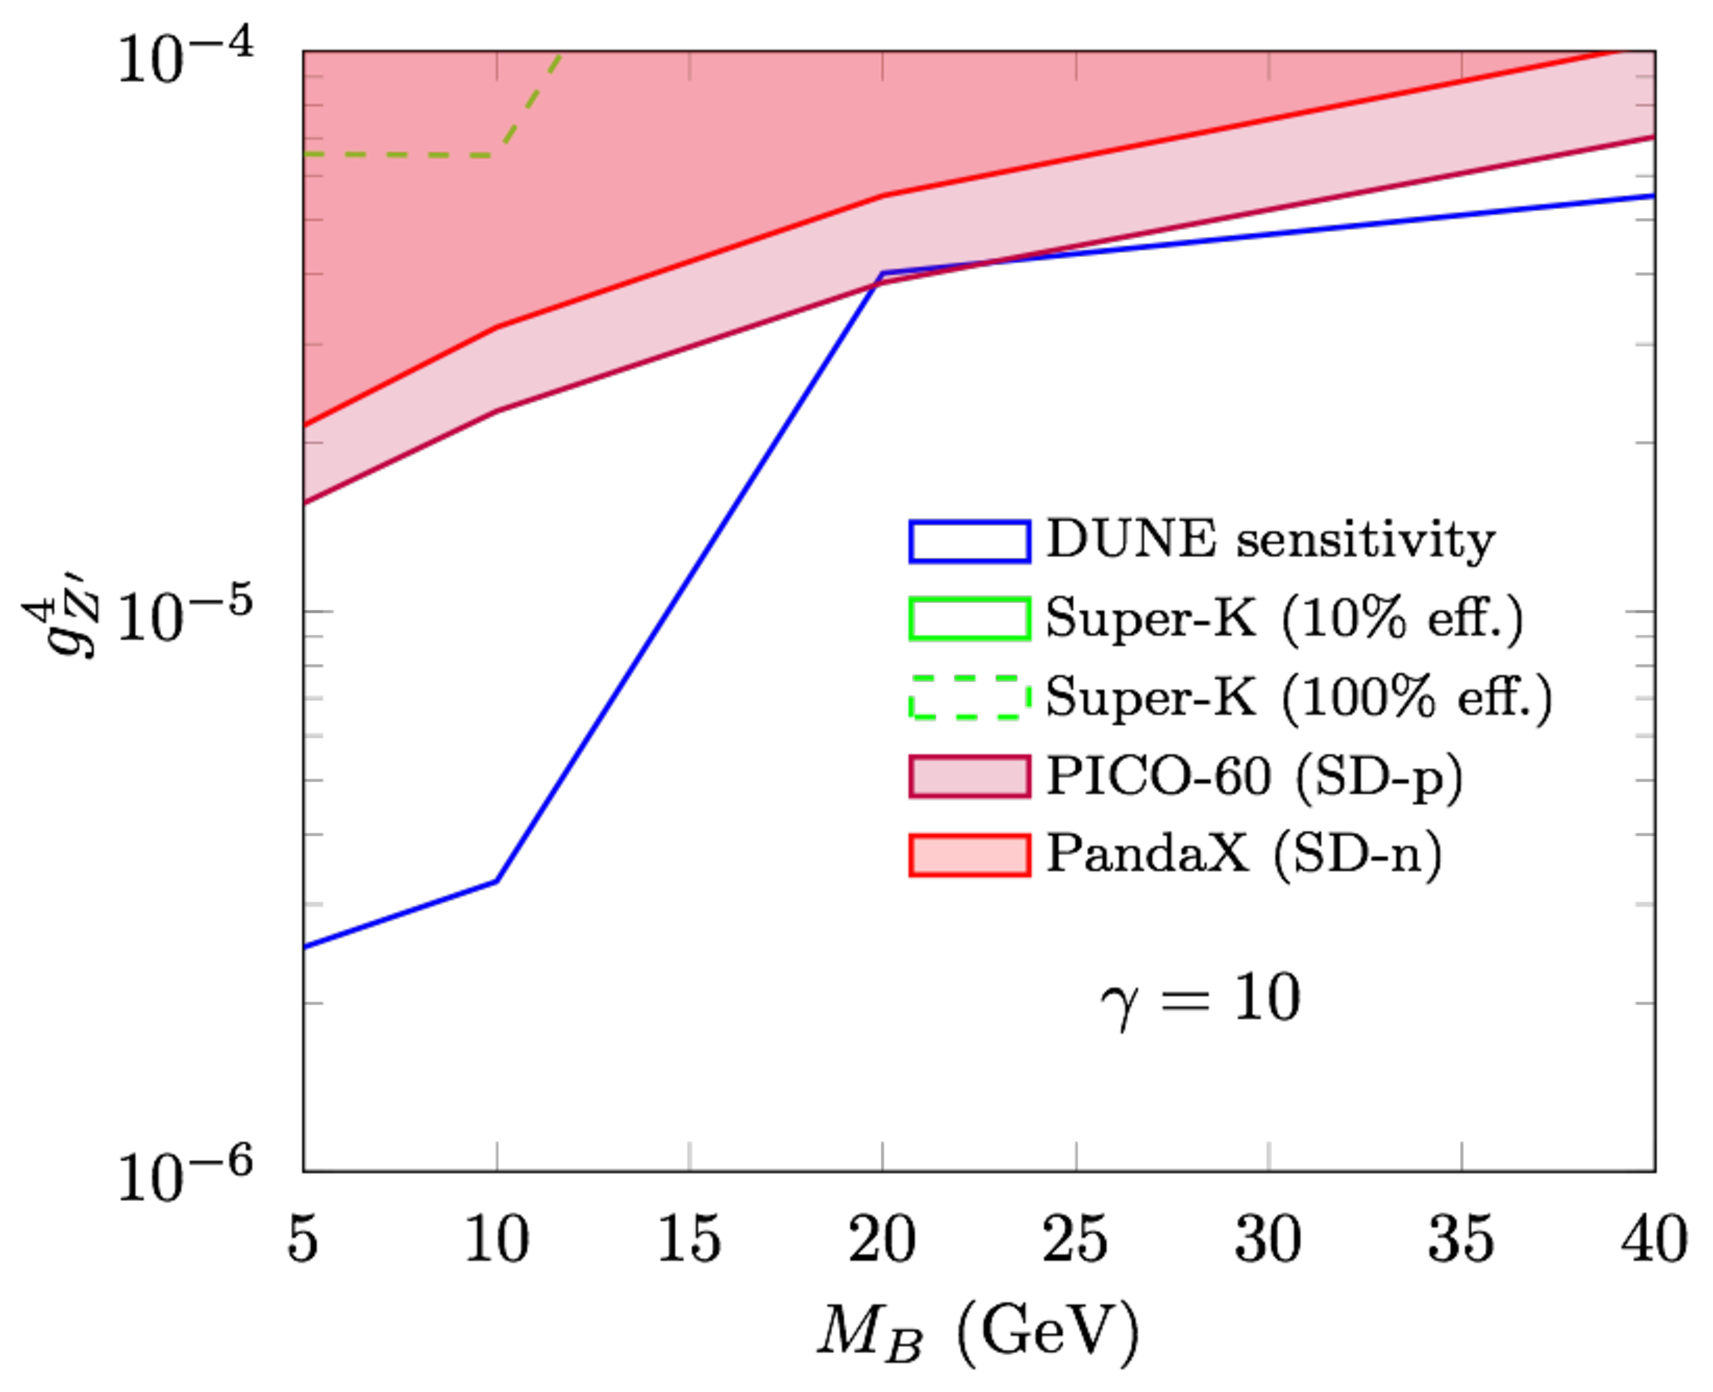
\includegraphics[width=0.45\textwidth]{bdm_preliminary_10_sa_legend}
\caption[Comparison of DUNE (10 yr) sensitivity to \superk sensitivity]{Comparison of sensitivity of DUNE for 10 years of data collection and 40~kton of detector mass with Super Kamiokande, assuming 10\% and 100\% of the selection efficiency on the atmospheric neutrino analysis in Ref.~\cite{Fechner:2009aa}, and with the reinterpretaions of the current results from PICO-60~\cite{Amole:2019fdf} and PandaX~\cite{Xia:2018qgs}.  The samples with two boosted factors, $\gamma = 1.25$ (left) and $\gamma = 10$ (right), are also presented. \label{fig:bdm_sensitivity_comparison}}
\end{figure*}
% -----------------------------------------------------------------------

%%%%%%%%%%%%%%%%%%%%%%%%%
\subsection{Discussion and Conclusions}

In this work, we have conducted simulation studies of the dark matter models described in eqs.~\eqref{eq:lagrangian} and \eqref{eq:zprimelag} in terms of their detection prospects at the DUNE \dword{nd} and \dword{fd}. 
Thanks to its relatively low threshold and strong particle identification capabilities, DUNE presents an opportunity to significantly advance the search for \dword{ldm} and \dword{bdm} beyond what has been possible with water Cherenkov detectors.

In the case of the \dword{nd}, we assumed that the relativistic \dword{dm} is being produced directly at the target and leaves an experimental signature through an elastic electron scattering. Using two constrained parameters of the light \dword{dm} model and a range of two free parameters, a sensitivity map was produced. Within the context of the vector portal \dword{dm} model and the chosen parameter constraints along with the electron scattering as the signal event, this result sets stringent limits on \dword{dm} parameters that are comparable or even better than recent experimental bounds in the sub-GeV mass range.

By contrast, in the case of the \dword{fd} modules, we assumed that the signal events are due to \dword{dm} coming from the galactic halo and the sun with a significant boost factor. 
For the \textit{in}elastic scattering case, the \dword{dm} scatters off either an electron or proton in the detector material into a heavier unstable dark-sector state.
%(i.e., \textit{in}elastic scattering). 
The heavier state, by construction, decays back to \dword{dm} and an electron-positron pair via a dark-photon exchange. 
Therefore, in the final state, a signal event comes with an electron or proton recoil plus an electron-positron pair. 
This distinctive signal feature enabled us to perform (almost) background-free analyses. 
As \dword{protodune} detectors are prototypes of DUNE \dword{fd} modules, the same study was conducted and corresponding results were compared with the ones of the DUNE \dword{fd} modules.  
We first investigated the experimental sensitivity in a dark-photon parameter space, dark-photon mass $m_V$ versus kinetic mixing parameter $\epsilon$. 
The results were shown separately for Scenario 1 and 2. 
They suggest that \dword{protodune} and DUNE \dword{fd} modules would probe a broad range of unexplored regions; they would allow for reaching $\sim 1-2$ orders of magnitude smaller $\epsilon$ values than the current limits along MeV to sub-GeV-range dark photons. 
We also examined model-independent reaches at both \dword{protodune} detectors and DUNE \dword{fd} modules, providing limits for models that assume the existence of $i$\dword{bdm} (or $i$\dword{bdm}-like) signals (i.e., a target recoil and a fermion pair). 

For the elastic scattering case, we considered the case in which \dword{bdm} comes from the sun. 
With one year of data, the $5\sigma$ sensitivity is expected to reach a coupling of $g_{Z^\prime}^4 = 9.57 \times 10^{-10}$ for a boost of 1.25 and $g_{Z^\prime}^4 = 1.49 \times 10^{-10}$ for a boost of 10 at a \dword{dm} mass of \SI{10}{GeV} without including neutrons in the reconstruction.



%%%%%%%%%%%%%%%%%%%%%%%%%%%%%%%%%%%%%%%%
\section{Other \dword{bsm} Physics Opportunities}
\label{sec:otheropps}

%%%%%%%%%%%%%%%%%%%%%%%%%
\subsection{Tau Neutrino Appearance} 



With only 19 $\nu_{\tau}$-\dword{cc} and $\bar{\nu}_{\tau}$-\dword{cc} candidates detected with high purity, we have less direct experimental knowledge of tau neutrinos than of any other \dword{sm} particle. Of these, nine $\nu_{\tau}$-\dword{cc} and $\bar{\nu}_{\tau}$-\dword{cc} candidate events with a background of 1.5 events, observed by the DONuT experiment~\cite{Kodama:2000mp, Kodama:2007aa}, were directly produced though $D_S$ meson decays.  The remaining 10 $\nu_{\tau}$-\dword{cc} candidate events with an estimated background of two events, observed by the OPERA experiment~\cite{Guler:2000bd,Agafonova:2018auq}, were produced through the oscillation of a muon neutrino beam. From this sample, a 20\% measurement of $\Delta m^{2}_{32}$ was performed under the assumption that $\sin^22\theta_{23} = 1$.  The \superk and IceCube experiments developed methods to statistically separate samples of $\nu_{\tau}$-\dword{cc} and $\bar{\nu}_{\tau}$-\dword{cc} events in atmospheric neutrinos to exclude the no-tau-neutrino appearance hypothesis at the 4.6$\sigma$ level and 3.2$\sigma$ level respectively~\cite{Abe:2012jj, Li:2017dbe, Aartsen:2019tjl}, but limitations of Cherenkov detectors constrain the ability to select a high-purity sample and perform precision measurements.



The DUNE experiment has the possibility of significantly improving the experimental situation. Tau-neutrino appearance can potentially improve the discovery potential for sterile neutrinos, \dword{nc} \dword{nsi}, and non-unitarity.  For model independence, the first goal should be measuring the atmospheric oscillation parameters in the $\nu_{\tau}$ appearance channel and checking the consistency of this measurement with those performed using the $\nu_{\mu}$ disappearance channel.  A truth-level study of $\nu_{\tau}$ selection in atmospheric neutrinos in a large, underground LArTPC detector suggested that $\nu_{\tau}$-\dword{cc} interactions with hadronically decaying $\tau$-leptons, which make up 65\% of total $\tau$-lepton decays~\cite{Tanabashi:2018oca}, can be selected with high purity~\cite{Conrad:1008}.  This analysis suggests that it may be possible to select up to 30\% of $\nu_{\tau}$-\dword{cc} events with hadronically decaying $\tau$-leptons with minimal neutral current background.  Under these assumptions, we expect to select $\sim$25 $\nu_{\tau}$-\dword{cc} candidates per year using the \dword{cpv} optimized beam. The physics reach of this sample has been studied in Ref.~\cite{deGouvea:2019ozk}. As shown in Figure~\ref{fig:nutauContours} (left), this sample is sufficient to simultaneously constrain $\Delta m^2_{31}$ and $\sin^22\theta_{23}$. Independent measurements of $\Delta m^2_{31}$ and $\sin^22\theta_{23}$ in the $\nu_{e}$ appearance, $\nu_{\mu}$ disappearance, and $\nu_{\tau}$ appearance channels should allow DUNE to constrain $|U_{e3}|^2+|U_{\mu 3}|^2+|U_{\tau 3}|^2$ to 6\%~\cite{deGouvea:2019ozk}, a significant improvement over current constraints~\cite{Parke:2015goa}.

\begin{figure}[!htb]
 \centering
        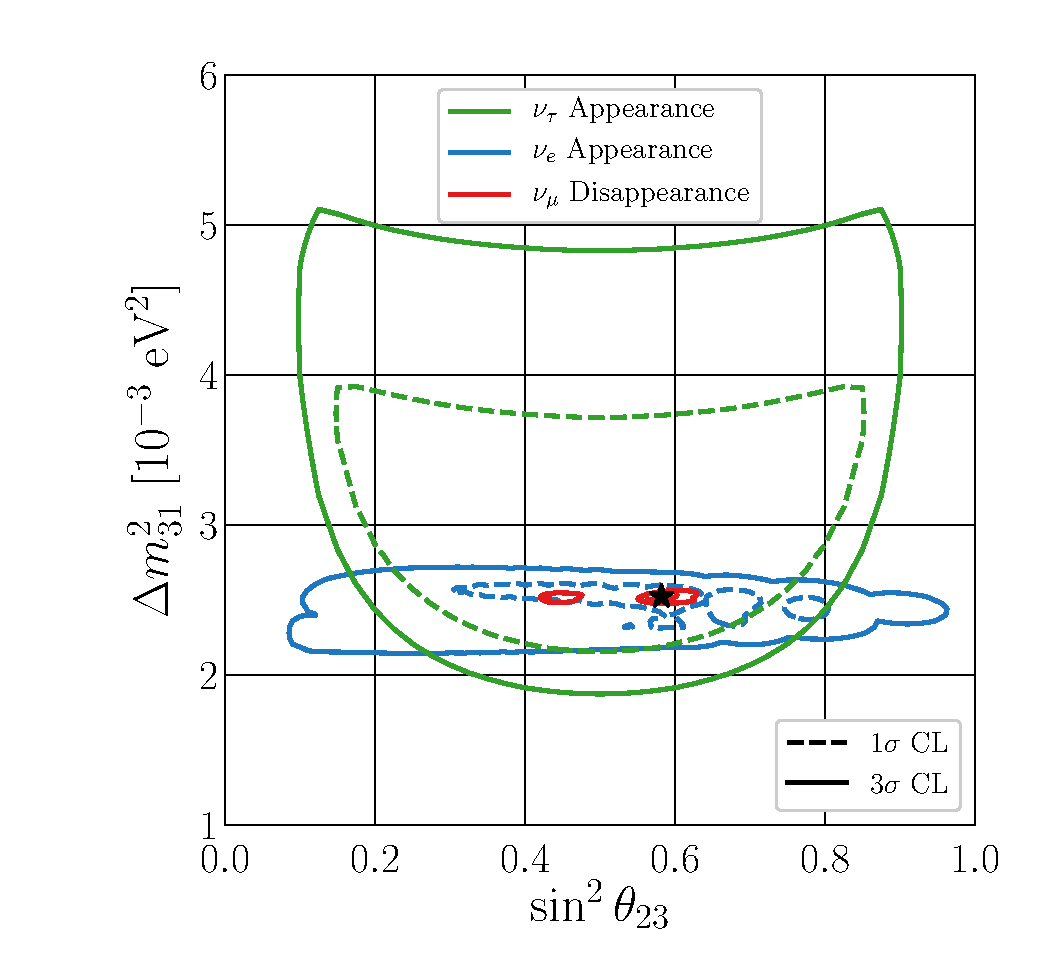
\includegraphics[width=0.4\columnwidth]{graphics/NuTauSensitivity_s23_dm31.pdf}
        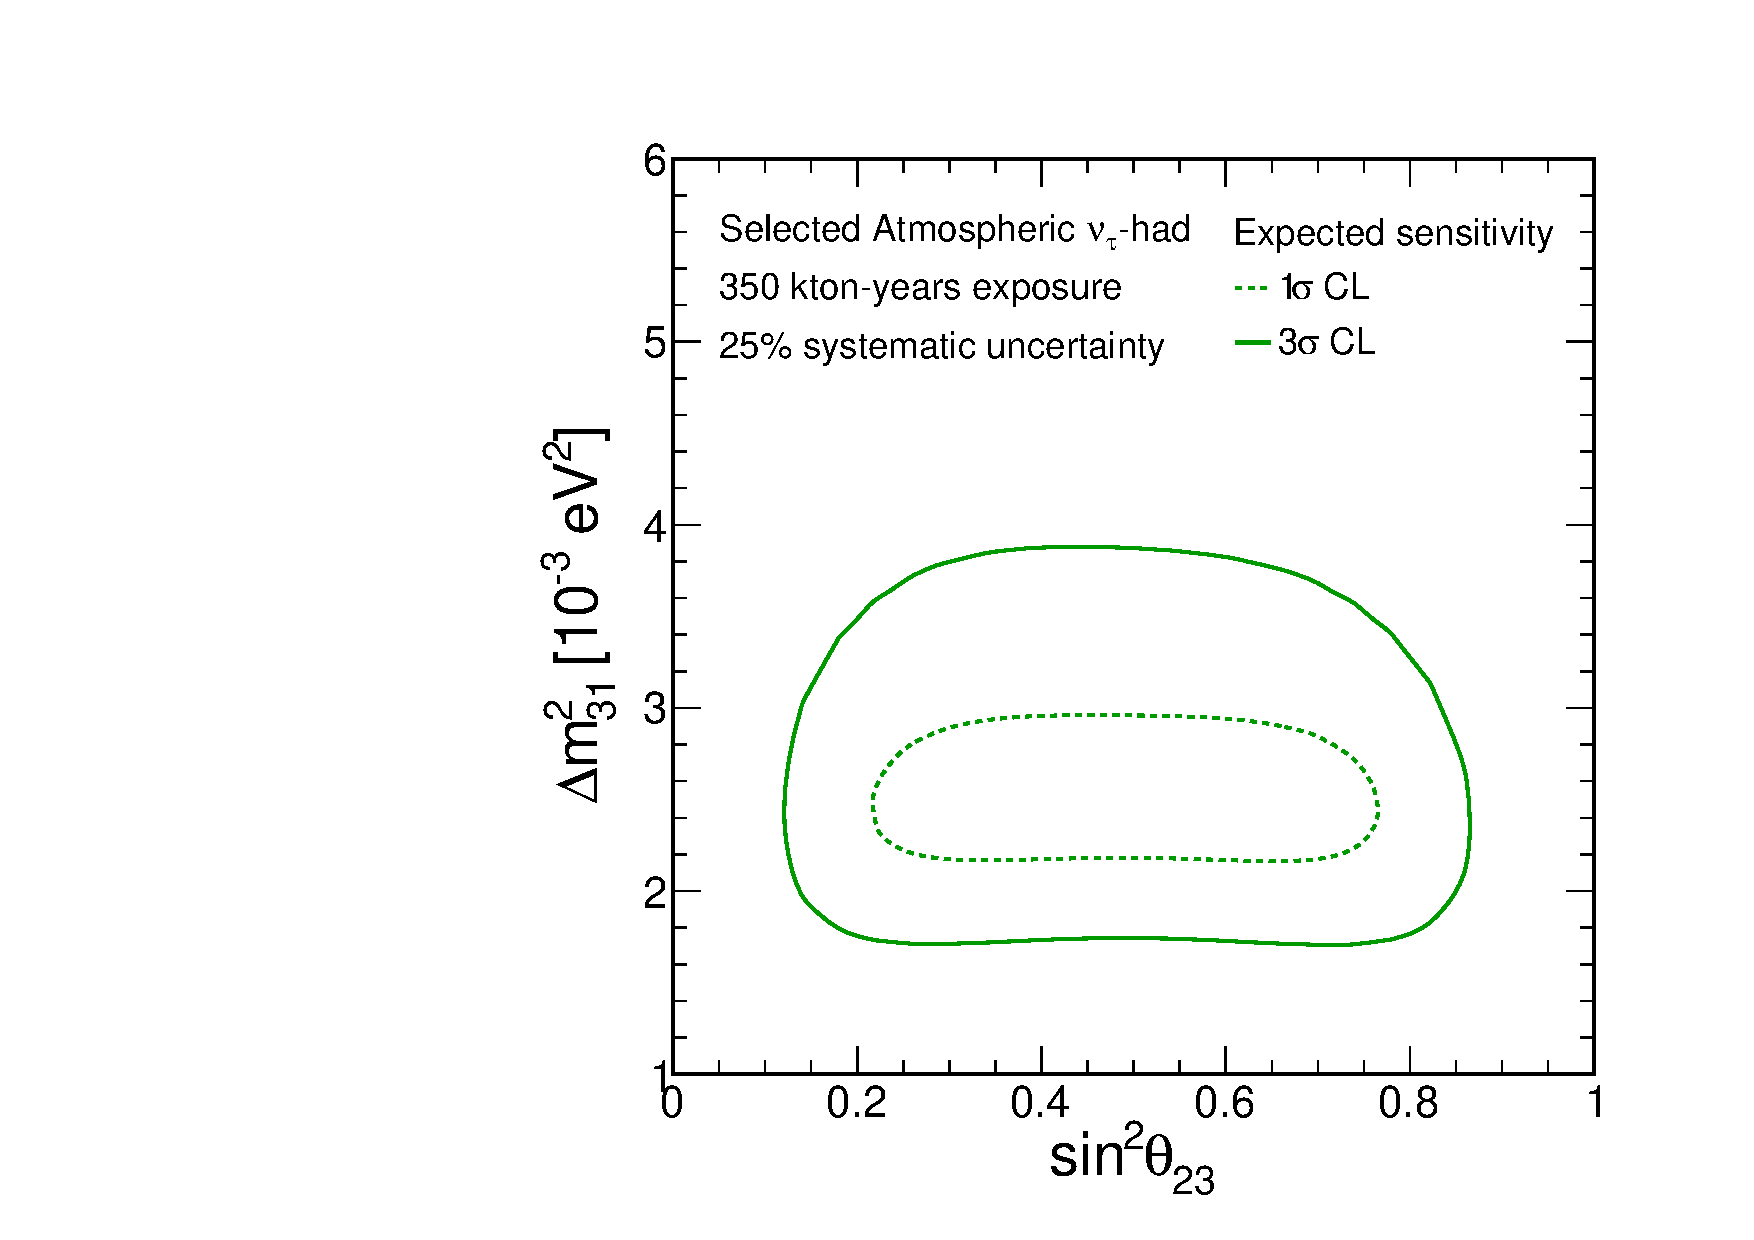
\includegraphics[width=0.4\columnwidth]{graphics/cAtmosNuTau.pdf}
	\caption[The 1$\sigma$ and 3$\sigma$ expected sensitivity for measuring $\Delta m^2_{31}$ and $\sin^2\theta_{23}$] % using a variety of samples.]
	{The 1$\sigma$ (dashed) and 3$\sigma$ (solid) expected sensitivity for measuring $\Delta m^2_{31}$ and $\sin^2\theta_{23}$ using a variety of samples. Left: The expected sensitivity for seven years of beam data collection, assuming 3.5 years each in neutrino and antineutrino modes, measured independently using $\nu_{e}$ appearance (blue), $\nu_{\mu}$ disappearance (red), and $\nu_{\tau}$ appearance (green). Adapted from Ref.~\cite{deGouvea:2019ozk}. Right: The expected sensitivity for the $\nu_{\tau}$ appearance channel using 350 kton-years of atmospheric exposure.}
	\label{fig:nutauContours}
\end{figure}

However, all of the events in the beam sample occur at energies higher than the first oscillation maximum due to kinematic constraints.  Only seeing the tail of the oscillation maximum creates a partial degeneracy between the measurement of $\Delta m^2_{31}$ and $\sin^22\theta_{23}$.  Atmospheric neutrinos, due to sampling a much larger $L/E$ range, allow for measuring both above and below the first oscillation maximum with $\nu_{\tau}$ appearance. Although we only expect to select $\sim$70 $\nu_{\tau}$-\dword{cc} and $\bar{\nu}_{\tau}$-\dword{cc} candidates in 350 kt-year in the atmospheric sample, as shown in Figure~\ref{fig:nutauContours} (right), a direct measurement of the oscillation maximum breaks the degeneracy seen in the beam sample. The complementary shapes of the beam and atmospheric constraints combine to reduce the uncertainty on $\sin^2\theta_{23}$, directly leading to improved unitarity constraints.  Finally, a high-energy beam option optimized for $\nu_{\tau}$ appearance should produce $\sim$150 selected  $\nu_{\tau}$-\dword{cc} candidates in one year.  These higher energy events are further in the tail of the first oscillation maximum, but they will permit a simultaneous measurement of the $\nu_{\tau}$ cross section. When analyzed within the non-unitarity framework described in Section~\ref{sec:nonUnitarity}, the high-energy beam significantly improves constraints on the parameter $\alpha_{33}$ due to increased matter effects~\cite{deGouvea:2019ozk}.

%%%%%%%%%%%%%%%%%%%%%%%%%
\subsection{Large Extra-Dimensions}
DUNE can search for or constrain the size of large extra-dimensions %(LED) 
by looking for distortions of the oscillation pattern predicted by the three-flavor paradigm. These distortions arise through mixing between the right-handed neutrino Kaluza-Klein modes, which propagate in the compactified extra dimensions, and the active neutrinos, which exist only in the four-dimensional brane~~\cite{Dienes:1998sb,ArkaniHamed:1998vp,Davoudiasl:2002fq}. Such distortions are determined by two parameters in the model, specifically R, the radius of the circle where the extra-dimension is compactified, and $m_0$, defined as the lightest active neutrino mass ($m_1$ for normal mass ordering, and $m_3$ for inverted mass ordering). Searching for these distortions in, for instance, the $\nu_\mu$~\dword{cc} disappearance spectrum, should provide significantly enhanced sensitivity over existing results from the MINOS/MINOS+ experiment~\cite{Adamson:2016yvy}.

%D.V.Forero (add text below)---------------------
\begin{figure}[ht]
\centerline{
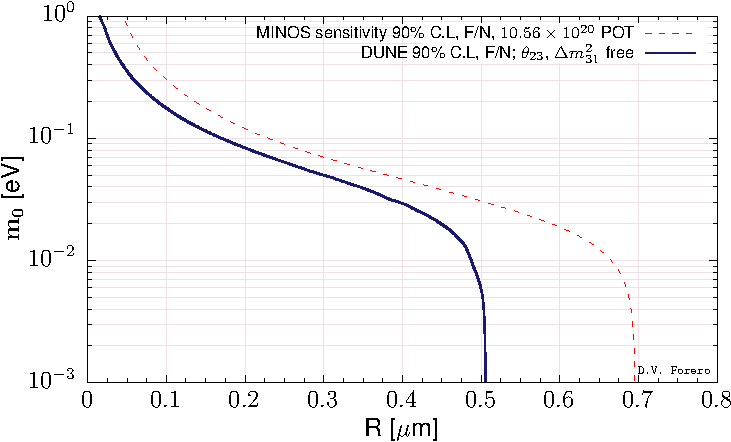
\includegraphics[width=0.7\textwidth]{graphics/LED_sensitivity.pdf}
}
\caption[DUNE sensitivity to the LED model]{Sensitivity to the LED model in Ref.~\cite{Dienes:1998sb,ArkaniHamed:1998vp,Davoudiasl:2002fq} through its impact on the neutrino oscillations expected at 
DUNE. For comparison, the MINOS sensitivity~\cite{Adamson:2016yvy} is also shown.}
\label{fig:ledsensitivity}
\end{figure}

Figure~\ref{fig:ledsensitivity} shows a comparison between the DUNE and MINOS~\cite{Adamson:2016yvy} 
sensitivities to LED at $90\%$ \dword{cl} for two degrees of freedom represented by the solid and dashed lines, respectively. 
In the case of DUNE, an exposure of $300\,\text{kt}\,\text{MW}\,\text{year}$ 
was assumed and spectral information from the four oscillation channels, (anti)neutrino 
appearance and disappearance, were included in the analysis. The muon (anti)neutrino 
fluxes, cross sections for the neutrino interactions in argon, detector energy 
resolutions, efficiencies and systematical errors were taken into account by the use of 
GLoBES files prepared for the DUNE LBL studies. In the analysis, we assumed DUNE 
simulated data as compatible with the standard three neutrino hypothesis (which corresponds to the limit $R\to 0$) and we have 
tested the LED model. The solar parameters were kept fixed, and also the reactor mixing 
angle, while the atmospheric parameters were allowed to float free. In general, DUNE 
improves over the MINOS sensitivity for all values of $m_0$ and this is more noticeable 
for $m_0\sim 10^{-3}$~eV, where the most conservative sensitivity limit to $R$ is 
obtained. 

%%%%%%%%%%%%%%%%%%%%%%%%%
\subsection{Heavy Neutral Leptons}
The high intensity of the LBNF neutrino beam and the production of charm and bottom mesons in the beam enables DUNE to search for a wide variety of lightweight long-lived, exotic particles, by looking for topologies of rare event interactions and decays in the fiducial volume of the DUNE \dword{nd}. These particles include weakly interacting heavy neutral leptons (HNLs), such as right-handed partners of the active neutrinos, light super-symmetric particles, or vector, scalar, and/or axion portals to a Hidden Sector containing new interactions and new particles. 
Assuming these heavy neutral leptons are the lighter particles of their hidden sector, they will only decay into \dword{sm} particles. The parameter space explored by the DUNE \dword{nd} extends into the cosmologically relevant region complementary to the LHC heavy-mass dark-matter searches through missing energy and mono-jets.

Thanks to small mixing angles, the particles can be stable enough to travel from the baseline to the detector and decay inside the active region.
It is worth noting that, differently from a light neutrino beam, an HNL beam is not polarised, due to their large mass.
The correct description of the helicity components in the beam is important for predicting the angular distributions
of HNL decays, as they might depend on the initial helicity state.
More specifically, there is a different phenomenology if the decaying HNL is a Majorana or a Dirac fermion~\cite{Balantekin:2018ukw, Ballett:2019bgd}.
Typical decay channels are two-body decays into a charged lepton and a pseudo-scalar meson, or a vector meson if
the mass allows it, two-body decays into neutral mesons, and three-body leptonic decays.

\begin{figure}[!htb]
	\begin{center}
	  	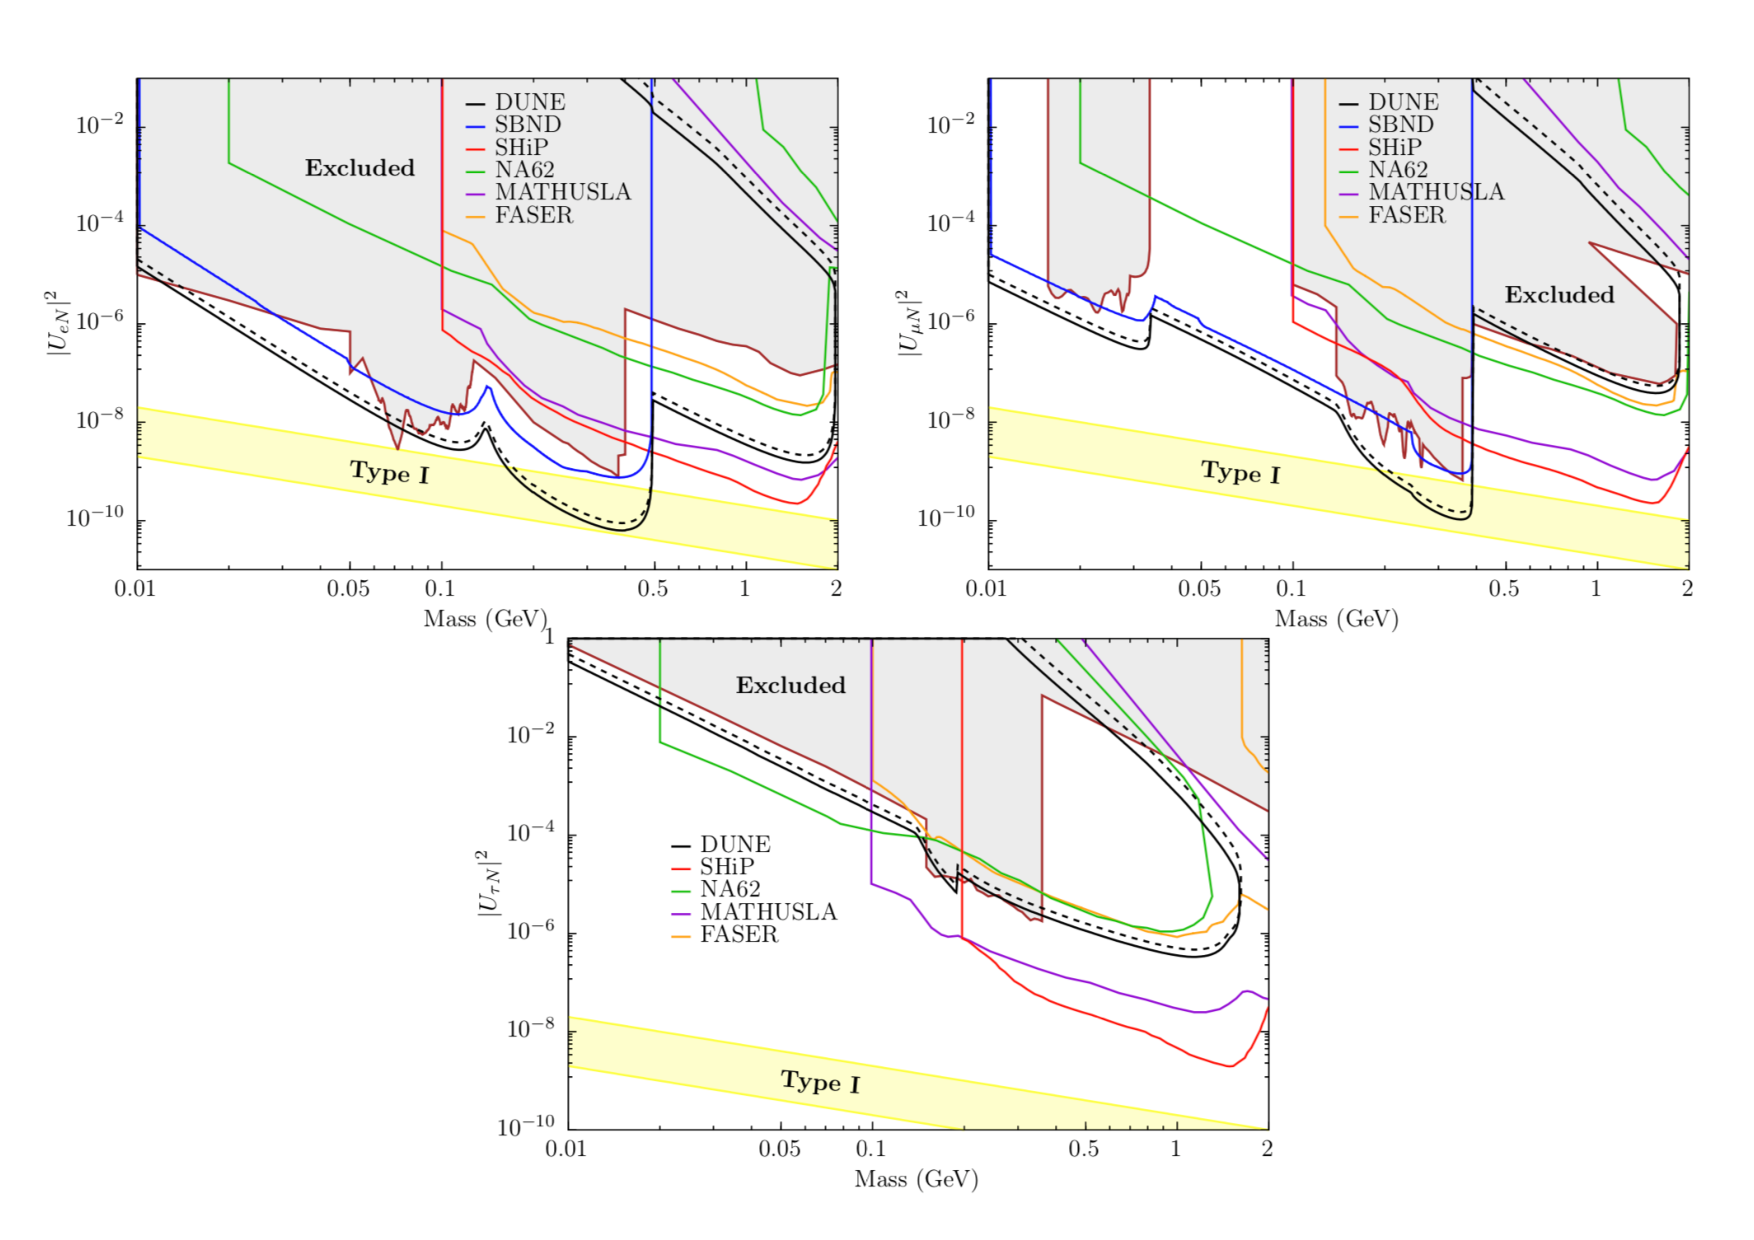
\includegraphics[width=0.73\textwidth]{graphics/DUNE_BSM_HNL.pdf}
	\end{center}
\caption[The 90\,\% \dword{cl} sensitivity regions for dominant mixings
		$|U_{\alpha N}|^2$]
		{The 90\,\% \dword{cl} sensitivity regions for dominant mixings %
		$|U_{e N}|^2$ (top~left), $|U_{\mu N}|^2$ (top right), and $|U_{\tau N}|^2$ (bottom) are presented for DUNE ND (black)~\cite{Ballett:2019bgd}.
		The regions are a combination of the sensitivity to HNL decay channels with good detection prospects.These are $N\to\nu e e$, $\nu e \mu$, $\nu \mu \mu$, $\nu \pi^0$, $e \pi$, and $\mu \pi$.The study is performed for Majorana neutrinos (solid) and Dirac neutrinos (dashed), %
		assuming no background. The region excluded by experimental constraints (grey/brown) is obtained by combining the results from PS191~\cite{Bernardi:1985ny, Bernardi:1987ek}, %
		peak searches~\cite{Artamonov:2014urb, Britton:1992pg, Britton:1992xv, Aguilar-Arevalo:2017vlf, Aguilar-Arevalo:2019owf}, %
		CHARM~\cite{Vilain:1994vg}, NuTeV~\cite{Vaitaitis:1999wq}, DELPHI~\cite{Abreu:1996pa}, and T2K~\cite{Abe:2019kgx}. The sensitivity for DUNE ND is compared to the predictions of future experiments, SBN~\cite{Ballett:2016opr} (blue), %
		SHiP~\cite{Alekhin:2015byh} (red), NA62~\cite{Drewes:2018gkc} (green), MATHUSLA~\cite{Curtin:2018mvb} (purple), and the Phase II of FASER~\cite{Kling:2018wct}.
		For reference, a band corresponding to the contribution light neutrino masses between 20~meV and 200~meV in a single generation see-saw type I model is shown (yellow).
		Larger values of the mixing angles are allowed if an extension to see-saw models is invoked,
		for instance, in an inverse or extended see-saw scheme.}
\label{fig:sensa_hnl}
\end{figure}

A recent study illustrates the potential sensitivity for  HNLs searches with the DUNE Near Detector~\cite{Ballett:2019bgd}. The sensitivity for HNL particles with masses in the range of 10 MeV to 2 GeV, from decays of mesons produced
in the proton beam dump that produces the pions for the neutrino beam production, was studied. The production
of $D_s$ mesons leads to access to high mass HNL production. The dominant HNL decay modes to SM particles
have been included, and basic detector constraints as well as the dominant background process have 
been taking into account. 

The experimental signature for these decays is a decay-in-flight event with no interaction vertex, typical of
neutrino--nucleon scattering, and a rather forward direction with respect to the beam.
The main background to this search comes from SM neutrino--nucleon scattering events in which the hadronic activity
at the vertex is below threshold.
Charged current quasi-elastic events with pion emission from resonances are background to the semi-leptonic decay channels,
whereas mis-identification of long pion tracks into muons can constitute a background to three-body leptonic decays.
Neutral pions are often emitted in neutrino scattering events and can be a challenge for decays into %
neutral meson or channels with electrons in the final state.

We report in Fig.~\ref{fig:sensa_hnl} the physics reach of the DUNE ND in its current configuration %
without backgrounds and for a Majorana and a Dirac HNL.
%We also point out that a significant number of $D_s$ mesons are produced thanks to the sufficiently high proton %energy of the beam.
The sensitivity was estimated assuming a total of 1.32 x $10^{22}$ POT, i.e. for a running scenario with 6 years with a 80 GeV proton beam of 1.2 MW, followed by six years of a beam with 2.4 MW, but using only the neutrino mode configuration, which corresponds to half of the total
runtime.
As a result, HNLs with masses up to 2 GeV can be searched for in all flavor-mixing channels.



The results show that DUNE will have an improved sensitivity to small values of the
mixing parameters $|U_{\alpha N}|^2$, where $\alpha=e,\,\mu,\,\tau$, compared to the presently available experimental
limits on mixing of HNLs with the three lepton flavors. At 90\% \dword{cl} sensitivity, DUNE can probe mixing parameters as low as 
$10^{-9}-10^{-10}$ in the mass range of 300-500 MeV, for  mixing with the electron or muon neutrino flavors. In the region above 500 MeV the sensitivity
is reduced to $10^{-8}$ for $eN$ mixing and $10^{-7}$ for $\mu N$ mixing. The $\tau N$ mixing 
sensitivity is weaker but still covering a new unexplored regime. A large fraction of the covered parameter space for all neutrino flavors falls in the region that is relevant for explaining the baryon asymmetry in the universe.

Studies are ongoing with full detector simulations to validate these 
encouraging results.


%%%%%%%%%%%%%%%%%%%%%%%%%
\subsection{Dark Matter Annihilation in the Sun}
DUNE's large \dword{fd} LArTPC modules provide an excellent setting to conduct searches for neutrinos arising from \dword{dm} annihilation in the core of the sun. These would typically result in a high-energy neutrino signal almost always accompanied by a low-energy neutrino component, which has its origin in a hadronic cascade that develops in the dense solar medium and produces large numbers of light long-lived mesons, such as $\pi^+$ and $K^+$ that
then stop and decay at rest. The decay of each $\pi^+$ and $K^+$ will produce monoenergetic neutrinos with an energy \SI{30}{MeV} or \SI{236}{MeV}, respectively.
The  \SI{236}{MeV} flux can be measured with the DUNE \dword{fd}, thanks to its excellent energy resolution, and importantly, will benefit from directional information. By selecting neutrinos arriving from the direction of the sun, large reduction in backgrounds can be achieved.
This directional resolution for sub-GeV neutrinos will enable DUNE to be competitive with experiments with even larger fiducial masses, but less precise angular information, such as Hyper-K~\cite{ref:DMannihilation}.

%%%%%%%%%%%%%%%%%%%%%%%%%%%%%%%%%%%%%%%%
\section{Conclusions and Outlook}
DUNE will be a powerful discovery tool on a variety of physics topics under very active exploration today, from the potential discovery of new particules beyond those predicted in the \dword{sm}, to precision neutrino measurements that may uncover deviations from the present three-flavor mixing paradigm and unveil new interactions and symmetries.
The \dword{nd} alone will offer excellent opportunities to search for light \dword{dm} and mixing with light sterile neutrinos, and to measure rare processes such as neutrino trident interactions. Besides looking for deviations from the three-flavor oscillation paradigm such as nonstandard interactions, DUNE's massive high-resolution \dword{fd} will probe the possible existence of \dword{bdm}. The flexibility of the LBNF beamline enables planning for high-energy beam running, providing access to probing and measuring tau neutrino physics with unprecedented precision.

DUNE will offer a long-term privileged setting for collaboration between experimentalists and theorists in the domain areas of neutrino physics, astrophysics, and cosmology, and will provide the highest potential for breakthrough discoveries among the new near-term facilities projected to start operations during the next decade.
